% Options for packages loaded elsewhere
\PassOptionsToPackage{unicode}{hyperref}
\PassOptionsToPackage{hyphens}{url}
\PassOptionsToPackage{dvipsnames,svgnames*,x11names*}{xcolor}
%
\documentclass[
]{book}
\usepackage{lmodern}
\usepackage{amssymb,amsmath}
\usepackage{ifxetex,ifluatex}
\ifnum 0\ifxetex 1\fi\ifluatex 1\fi=0 % if pdftex
  \usepackage[T1]{fontenc}
  \usepackage[utf8]{inputenc}
  \usepackage{textcomp} % provide euro and other symbols
\else % if luatex or xetex
  \usepackage{unicode-math}
  \defaultfontfeatures{Scale=MatchLowercase}
  \defaultfontfeatures[\rmfamily]{Ligatures=TeX,Scale=1}
\fi
% Use upquote if available, for straight quotes in verbatim environments
\IfFileExists{upquote.sty}{\usepackage{upquote}}{}
\IfFileExists{microtype.sty}{% use microtype if available
  \usepackage[]{microtype}
  \UseMicrotypeSet[protrusion]{basicmath} % disable protrusion for tt fonts
}{}
\makeatletter
\@ifundefined{KOMAClassName}{% if non-KOMA class
  \IfFileExists{parskip.sty}{%
    \usepackage{parskip}
  }{% else
    \setlength{\parindent}{0pt}
    \setlength{\parskip}{6pt plus 2pt minus 1pt}}
}{% if KOMA class
  \KOMAoptions{parskip=half}}
\makeatother
\usepackage{xcolor}
\IfFileExists{xurl.sty}{\usepackage{xurl}}{} % add URL line breaks if available
\IfFileExists{bookmark.sty}{\usepackage{bookmark}}{\usepackage{hyperref}}
\hypersetup{
  pdftitle={Numerik des Maschinellen Lernens},
  pdfauthor={Jan Heiland},
  colorlinks=true,
  linkcolor=Maroon,
  filecolor=Maroon,
  citecolor=Blue,
  urlcolor=purple,
  pdfcreator={LaTeX via pandoc}}
\urlstyle{same} % disable monospaced font for URLs
\usepackage{color}
\usepackage{fancyvrb}
\newcommand{\VerbBar}{|}
\newcommand{\VERB}{\Verb[commandchars=\\\{\}]}
\DefineVerbatimEnvironment{Highlighting}{Verbatim}{commandchars=\\\{\}}
% Add ',fontsize=\small' for more characters per line
\usepackage{framed}
\definecolor{shadecolor}{RGB}{248,248,248}
\newenvironment{Shaded}{\begin{snugshade}}{\end{snugshade}}
\newcommand{\AlertTok}[1]{\textcolor[rgb]{0.94,0.16,0.16}{#1}}
\newcommand{\AnnotationTok}[1]{\textcolor[rgb]{0.56,0.35,0.01}{\textbf{\textit{#1}}}}
\newcommand{\AttributeTok}[1]{\textcolor[rgb]{0.77,0.63,0.00}{#1}}
\newcommand{\BaseNTok}[1]{\textcolor[rgb]{0.00,0.00,0.81}{#1}}
\newcommand{\BuiltInTok}[1]{#1}
\newcommand{\CharTok}[1]{\textcolor[rgb]{0.31,0.60,0.02}{#1}}
\newcommand{\CommentTok}[1]{\textcolor[rgb]{0.56,0.35,0.01}{\textit{#1}}}
\newcommand{\CommentVarTok}[1]{\textcolor[rgb]{0.56,0.35,0.01}{\textbf{\textit{#1}}}}
\newcommand{\ConstantTok}[1]{\textcolor[rgb]{0.00,0.00,0.00}{#1}}
\newcommand{\ControlFlowTok}[1]{\textcolor[rgb]{0.13,0.29,0.53}{\textbf{#1}}}
\newcommand{\DataTypeTok}[1]{\textcolor[rgb]{0.13,0.29,0.53}{#1}}
\newcommand{\DecValTok}[1]{\textcolor[rgb]{0.00,0.00,0.81}{#1}}
\newcommand{\DocumentationTok}[1]{\textcolor[rgb]{0.56,0.35,0.01}{\textbf{\textit{#1}}}}
\newcommand{\ErrorTok}[1]{\textcolor[rgb]{0.64,0.00,0.00}{\textbf{#1}}}
\newcommand{\ExtensionTok}[1]{#1}
\newcommand{\FloatTok}[1]{\textcolor[rgb]{0.00,0.00,0.81}{#1}}
\newcommand{\FunctionTok}[1]{\textcolor[rgb]{0.00,0.00,0.00}{#1}}
\newcommand{\ImportTok}[1]{#1}
\newcommand{\InformationTok}[1]{\textcolor[rgb]{0.56,0.35,0.01}{\textbf{\textit{#1}}}}
\newcommand{\KeywordTok}[1]{\textcolor[rgb]{0.13,0.29,0.53}{\textbf{#1}}}
\newcommand{\NormalTok}[1]{#1}
\newcommand{\OperatorTok}[1]{\textcolor[rgb]{0.81,0.36,0.00}{\textbf{#1}}}
\newcommand{\OtherTok}[1]{\textcolor[rgb]{0.56,0.35,0.01}{#1}}
\newcommand{\PreprocessorTok}[1]{\textcolor[rgb]{0.56,0.35,0.01}{\textit{#1}}}
\newcommand{\RegionMarkerTok}[1]{#1}
\newcommand{\SpecialCharTok}[1]{\textcolor[rgb]{0.00,0.00,0.00}{#1}}
\newcommand{\SpecialStringTok}[1]{\textcolor[rgb]{0.31,0.60,0.02}{#1}}
\newcommand{\StringTok}[1]{\textcolor[rgb]{0.31,0.60,0.02}{#1}}
\newcommand{\VariableTok}[1]{\textcolor[rgb]{0.00,0.00,0.00}{#1}}
\newcommand{\VerbatimStringTok}[1]{\textcolor[rgb]{0.31,0.60,0.02}{#1}}
\newcommand{\WarningTok}[1]{\textcolor[rgb]{0.56,0.35,0.01}{\textbf{\textit{#1}}}}
\usepackage{longtable,booktabs}
% Correct order of tables after \paragraph or \subparagraph
\usepackage{etoolbox}
\makeatletter
\patchcmd\longtable{\par}{\if@noskipsec\mbox{}\fi\par}{}{}
\makeatother
% Allow footnotes in longtable head/foot
\IfFileExists{footnotehyper.sty}{\usepackage{footnotehyper}}{\usepackage{footnote}}
\makesavenoteenv{longtable}
\usepackage{graphicx}
\makeatletter
\def\maxwidth{\ifdim\Gin@nat@width>\linewidth\linewidth\else\Gin@nat@width\fi}
\def\maxheight{\ifdim\Gin@nat@height>\textheight\textheight\else\Gin@nat@height\fi}
\makeatother
% Scale images if necessary, so that they will not overflow the page
% margins by default, and it is still possible to overwrite the defaults
% using explicit options in \includegraphics[width, height, ...]{}
\setkeys{Gin}{width=\maxwidth,height=\maxheight,keepaspectratio}
% Set default figure placement to htbp
\makeatletter
\def\fps@figure{htbp}
\makeatother
\setlength{\emergencystretch}{3em} % prevent overfull lines
\providecommand{\tightlist}{%
  \setlength{\itemsep}{0pt}\setlength{\parskip}{0pt}}
\setcounter{secnumdepth}{5}
\usepackage{xcolor}
\definecolor{jhsc}{HTML}{1f57c7}
\newenvironment {JHSAYS} [0] {\begin{quote}\color{jhsc}} {\end{quote}}
\newlength{\cslhangindent}
\setlength{\cslhangindent}{1.5em}
\newenvironment{cslreferences}%
  {}%
  {\par}

\title{Numerik des Maschinellen Lernens}
\author{Jan Heiland}
\date{TU Ilmenau -- Sommersemester 2024}

\usepackage{amsthm}
\newtheorem{theorem}{Theorem}[chapter]
\newtheorem{lemma}{Lemma}[chapter]
\newtheorem{corollary}{Corollary}[chapter]
\newtheorem{proposition}{Proposition}[chapter]
\newtheorem{conjecture}{Conjecture}[chapter]
\theoremstyle{definition}
\newtheorem{definition}{Definition}[chapter]
\theoremstyle{definition}
\newtheorem{example}{Example}[chapter]
\theoremstyle{definition}
\newtheorem{exercise}{Exercise}[chapter]
\theoremstyle{definition}
\newtheorem{hypothesis}{Hypothesis}[chapter]
\theoremstyle{remark}
\newtheorem*{remark}{Remark}
\newtheorem*{solution}{Solution}
\begin{document}
\maketitle

{
\hypersetup{linkcolor=}
\setcounter{tocdepth}{1}
\tableofcontents
}
\hypertarget{vorwort}{%
\chapter*{Vorwort}\label{vorwort}}
\addcontentsline{toc}{chapter}{Vorwort}

Das ist ein Aufschrieb der parallel zur Vorlesung erweitert wird.

Korrekturen und Wünsche immer gerne als \emph{issues} oder \emph{pull requests} ans \href{https://github.com/highlando/script-ndml}{github-repo}.

\hypertarget{einfuxfchrung}{%
\chapter{Einführung}\label{einfuxfchrung}}

Was sind \emph{Numerische Methoden für Maschinelles Lernen} (ML)?

Kurz gesagt, beim Training eines ML-Modells durchläuft ein Computer Millionen von Anweisungen, die in Form mathematischer Ausdrücke formuliert sind. Gleiches gilt für die Bewertung eines solchen Modells.
Dann stellen sich Fragen wie \emph{wird es einen Punkt geben, an dem das Training endet?} und \emph{wird das Modell genau sein?}.

Um zu beschreiben, was passiert, und für die spätere Analyse führen wir die allgemeinen Konzepte von

\begin{itemize}
\tightlist
\item
  Algorithmus
\item
  Konsistenz/Genauigkeit
\item
  Stabilität
\item
  Rechenaufwand
\end{itemize}

ein, von denen einige klassische \emph{numerische Analysis} sind.

\hypertarget{was-ist-ein-algorithmus}{%
\section{Was ist ein Algorithmus}\label{was-ist-ein-algorithmus}}

Interessanterweise ist der Begriff \emph{Algorithmus} zugleich intuitiv und abstrakt. Es bedurfte großer Anstrengungen, um eine allgemeine und wohlgestellte Definition zu finden, die den Anforderungen und Einschränkungen aller Bereiche gerecht wird (von \emph{Kochrezepten} bis zur Analyse von \emph{formalen Sprachen}).

\begin{definition}[Algorithmus]
\protect\hypertarget{def:algorithm}{}\label{def:algorithm}Ein Problemlösungsverfahren wird als \emph{Algorithmus} bezeichnet, genau dann wenn es eine \emph{Turing-Maschine} gibt, die dem Verfahren entspricht und die, für jede Eingabe, für die eine Lösung existiert, \emph{anhalten} wird.
\end{definition}

Diese Definition ist in ihrer Allgemeinheit nicht allzu hilfreich - wir haben noch nicht einmal definiert, was eine Turing-Maschine ist.

\leavevmode\hypertarget{rem-coors}{}%
\begin{JHSAYS}
Eine \emph{Turing-Maschine} kann als eine Maschine beschrieben werden, die ein Band von Anweisungen liest und auf dieses Band schreiben kann. Abhängig davon, was sie liest, kann sie vorwärts bewegen, rückwärts bewegen oder anhalten (wenn das Band einen vordefinierten Zustand erreicht hat). Das Schöne daran ist, dass dieses Setup in einen vollständig mathematischen Rahmen gestellt werden kann.

\end{JHSAYS}

Hilfreicher und gebräuchlicher ist es, die Implikationen dieser Definition zu betrachten, um zu überprüfen, ob ein Verfahren zumindest die notwendigen Bedingungen für einen Algorithmus erfüllt

\begin{itemize}
\tightlist
\item
  Der Algorithmus wird durch endlich viele Anweisungen beschrieben (Endlichkeit).
\item
  Jeder Schritt ist \emph{durchführbar}.
\item
  Der Algorithmus erfordert eine endliche Menge an Speicher.
\item
  Er wird nach endlich vielen Schritten beendet.
\item
  In jedem Schritt ist der nächste Schritt eindeutig definiert (\emph{Determiniertheit}).
\item
  Für denselben Anfangszustand wird er im selben Endzustand anhalten (\emph{Bestimmtheit}).
\end{itemize}

Somit könnte eine informelle, gute Praxisdefinition eines Algorithmus sein

\begin{definition}[Algorithmus -- informell]
\protect\hypertarget{def:info-algorithm}{}\label{def:info-algorithm}Ein Verfahren aus endlich vielen Anweisungen wird als \emph{Algorithmus} bezeichnet, wenn es eine bestimmte Lösung -- falls sie existiert -- zu einem Problem in endlich vielen Schritten berechnet.
\end{definition}

\leavevmode\hypertarget{rem-algo-annahmen}{}%
\begin{JHSAYS}
Beachten Sie, wie einige Eigenschaften (wie endlich viele Anweisungen) a priori angenommen werden.

\end{JHSAYS}

Als informellere Verweise auf Algorithmen werden wir die Begriffe \textbf{\emph{(numerische) Methode}} oder \textbf{\emph{Schema}} verwenden, um ein Verfahren durch Auflistung seiner zugrundeliegenden Ideen und Unterprozeduren anzusprechen, wobei \emph{Algorithmus} sich auf eine spezifische Realisierung einer \emph{Methode} bezieht.

Weiterhin unterscheiden wir

\begin{itemize}
\tightlist
\item
  \emph{direkte} Methoden -- die die Lösung exakt berechnen (wie die Lösung eines linearen Systems durch \emph{Gauß-Elimination}) und
\item
  \emph{iterative} Methoden -- die iterativ eine Folge von Annäherungen an die Lösung berechnen (wie die Berechnung von Wurzeln mit einem \emph{Newton-Schema}).
\end{itemize}

\hypertarget{konsistenz-stabilituxe4t-genauigkeit}{%
\section{Konsistenz, Stabilität, Genauigkeit}\label{konsistenz-stabilituxe4t-genauigkeit}}

Für die Analyse numerischer Methoden werden allgemein die folgenden Begriffe verwendet:

\begin{definition}[Konsistenz]
\protect\hypertarget{def:consistency}{}\label{def:consistency}Wenn ein Algorithmus in exakter Arithmetik die Lösung des Problems mit einer gegebenen Genauigkeit berechnet, wird er als \emph{konsistent} bezeichnet.
\end{definition}

\begin{definition}[Stabilität (informell)]
\protect\hypertarget{def:stability}{}\label{def:stability}Wenn die Ausgabe eines Algorithmus kontinuierlich von Unterschieden in der Eingabe und kontinuierlich von Unterschieden in den Anweisungen abhängt, dann wird der Algorithmus als \emph{stabil} bezeichnet.
\end{definition}

Die \emph{Unterschiede in den Anweisungen} sind typischerweise auf Rundungsfehler zurückzuführen, wie sie in \emph{ungenauer Arithmetik} (oft auch als \emph{Gleitkommaarithmetik} bezeichnet) auftreten.

\leavevmode\hypertarget{rem-algo-kons-stab}{}%
\begin{JHSAYS}
Man könnte sagen, dass ein Algorithmus konsistent ist, wenn \emph{er das Richtige tut} und dass er stabil ist, \emph{wenn er trotz beliebiger kleiner Ungenauigkeiten funktioniert}. Wenn ein Algorithmus konsistent und stabil ist, wird er oft als \emph{konvergent} bezeichnet, um auszudrücken, dass er schließlich die Lösung auch in ungenauer Arithmetik berechnen wird.

\end{JHSAYS}

Beachten Sie, dass Begriffe wie

\begin{itemize}
\tightlist
\item
  \emph{Genauigkeit} -- wie nahe die berechnete Ausgabe der tatsächlichen Lösung kommt oder
\item
  \emph{Konvergenz} -- wie schnell (typischerweise in Bezug auf den Rechenaufwand) der Algorithmus sich der tatsächlichen Lösung nähert
\end{itemize}

keine intrinsischen Eigenschaften eines Algorithmus sind, da sie von dem zu lösenden Problem abhängen.
Man kann jedoch von \emph{Konsistenzordnung} eines Algorithmus sprechen, um die erwartete Genauigkeit für eine Klasse von Problemen zu spezifizieren, und einen Algorithmus als konvergent einer bestimmten Ordnung bezeichnen, wenn er zusätzlich stabil ist.

\hypertarget{rechenkomplexituxe4t}{%
\section{Rechenkomplexität}\label{rechenkomplexituxe4t}}

Die \emph{Rechenkomplexität} eines Algorithmus ist sowohl theoretisch (um abzuschätzen, wie der Aufwand mit beispielsweise der Größe des Problems skaliert) als auch praktisch (um zu sagen, wie lange das Verfahren dauern wird und welche Kosten in Bezug auf CPU-Zeit oder Speichernutzung es generieren wird) wichtig.

Typischerweise wird die Komplexität durch Zählen der elementaren Operationen gemessen -- wir werden stets die Ausführung einer Grundrechenart als eine Operation zählen.

\leavevmode\hypertarget{rem-flops}{}%
\begin{JHSAYS}
Die Definition einer \emph{elementaren Operation} auf einem Computer ist nicht universal, da viele Faktoren hier reinspielen. Gerne werden \emph{FLOP}
s angeführt, was für \emph{floating point operations} steht. Allerdings ist es wiederum sehr verschieden auf verschiedenen Prozessoren wieviele FLOPs für eine Multiplikation oder Addition gebraucht werden.

\end{JHSAYS}

Um die Algorithmen in Bezug auf Komplexität versus Problemgröße zu klassifizieren, sind die folgenden Funktionsklassen hilfreich

\begin{definition}[Landau-Symbole oder große O-Notation]
\protect\hypertarget{def:landau-symbs}{}\label{def:landau-symbs}Sei \(g\colon \mathbb R^{} \to \mathbb R^{}\) und \(a\in\mathbb R^{} \cup \{-\infty, +\infty\}\). Dann sagen wir für eine Funktion \(f\colon \mathbb R \to \mathbb R^{}\), dass \(f\in O(g)\), wenn
\begin{equation*}
\limsup_{x\to a} \frac{|f(x)|}{|g(x)|} < \infty
\end{equation*}
und dass \(f\in o(g)\), wenn
\begin{equation*}
\limsup_{x\to a} \frac{|f(x)|}{|g(x)|} = 0.
\end{equation*}
\end{definition}

Der Sinn und die Funktionalität dieser Konzepte wird vielleicht deutlich, wenn man sich die typischen Anwendungen ansieht:

\begin{itemize}
\tightlist
\item
  Wenn \(h> 0\) ein Diskretisierungsparameter ist und, sagen wir, \(e(h)\) der Diskretisierungsfehler ist, dann könnten wir sagen, dass \(e(h) = O(h^2)\), wenn \emph{asymptotisch}, d.h. für immer kleinere \(h\), der Fehler mindestens so schnell wie \(h^2\) gegen \(0\) geht.
\item
  Wenn \(C(n)\) die Komplexität eines Algorithmus für eine Problemgröße \(n\) ist, dann könnten wir sagen, dass \(C(n) = O(n)\), um auszudrücken, dass die Komplexität \emph{asymptotisch}, d.h. für immer größere \(n\), mit derselben Geschwindigkeit wie die Problemgröße wächst.
\end{itemize}

Leider ist die übliche Verwendung der Landau-Symbole etwas unpräzise.

\begin{enumerate}
\def\labelenumi{\arabic{enumi}.}
\tightlist
\item
  Das oft verwendete ``\(=\)''-Zeichen ist informell und keineswegs eine Gleichheit.
\item
  Was der Grenzwert \(a\) ist, wird selten explizit erwähnt, aber glücklicherweise ist es in der Regel aus dem Kontext klar.
\end{enumerate}

Als Beispiel betrachten wir zwei verschiedene Wege, ein Polynom \(p\) vom Grad \(n\) an der Abszisse \(x\) auszuwerten, basierend auf den zwei äquivalenten Darstellungen
\begin{equation*}
\begin{split}
p(x) &= a_0 + a_1x +  a_2x^2+ \dotsm + a_nx^n \\
     &= a_0 + x(a_1 + x(a_2 + \dotsm +x(a_{n-1} + a_nx) \dotsm ))
\end{split}
\end{equation*}

Für eine direkte Implementierung der ersten Darstellung erhalten wir die Algorithmen

\begin{Shaded}
\begin{Highlighting}[]
\CommentTok{\textquotesingle{}\textquotesingle{}\textquotesingle{}Berechnung von p(x) in Standarddarstellung}
\CommentTok{\textquotesingle{}\textquotesingle{}\textquotesingle{}}
\NormalTok{n }\OperatorTok{=} \DecValTok{10}                                      \CommentTok{\# Beispielwert für n}
\NormalTok{ais }\OperatorTok{=}\NormalTok{ [(}\OperatorTok{{-}}\DecValTok{1}\NormalTok{)}\OperatorTok{**}\NormalTok{k}\OperatorTok{*}\DecValTok{1}\OperatorTok{/}\NormalTok{k }\ControlFlowTok{for}\NormalTok{ k }\KeywordTok{in} \BuiltInTok{range}\NormalTok{(}\DecValTok{1}\NormalTok{, n}\OperatorTok{+}\DecValTok{2}\NormalTok{)]  }\CommentTok{\# Liste der Beispielkoeffizienten}
\NormalTok{x }\OperatorTok{=} \DecValTok{5}                                       \CommentTok{\# Ein Beispielwert für x}
\NormalTok{cpx }\OperatorTok{=}\NormalTok{ ais[}\DecValTok{0}\NormalTok{]                                }\CommentTok{\# der Fall k=0}
\ControlFlowTok{for}\NormalTok{ k }\KeywordTok{in} \BuiltInTok{range}\NormalTok{(n):}
\NormalTok{    cpx }\OperatorTok{=}\NormalTok{ cpx }\OperatorTok{+}\NormalTok{ ais[k}\OperatorTok{+}\DecValTok{1}\NormalTok{] }\OperatorTok{*}\NormalTok{ x}\OperatorTok{**}\NormalTok{(k}\OperatorTok{+}\DecValTok{1}\NormalTok{)         }\CommentTok{\# der Beitrag des k{-}ten Schritts}
\BuiltInTok{print}\NormalTok{(}\SpecialStringTok{f\textquotesingle{}x=}\SpecialCharTok{\{x\}}\SpecialStringTok{: p(x)=}\SpecialCharTok{\{}\NormalTok{cpx}\SpecialCharTok{:.4f\}}\SpecialStringTok{\textquotesingle{}}\NormalTok{)             }\CommentTok{\# Ausgabe des Ergebnisses}
\end{Highlighting}
\end{Shaded}

Im \(k\)-ten Schritt benötigt der Algorithmus eine Addition (wenn wir auch die Initialisierung als Addition zählen) und \(k\) Multiplikationen. Das ergibt eine Gesamtkomplexität von
\begin{equation*}
C(n) = \sum_{k=0}^n(1+k) = n+1 + \frac{n(n-1)}{2} = 1 + \frac n2 + \frac{n^2}2 = O(n^2)
\end{equation*}

Für die zweite Darstellung können wir das sogenannte \emph{Horner-Schema} implementieren, das lauten würde

\begin{Shaded}
\begin{Highlighting}[]
\CommentTok{\textquotesingle{}\textquotesingle{}\textquotesingle{}Berechnung von p(x) mit dem Horner{-}Schema}
\CommentTok{\textquotesingle{}\textquotesingle{}\textquotesingle{}}
\NormalTok{n }\OperatorTok{=} \DecValTok{10}                                      \CommentTok{\# Beispielwert für n}
\NormalTok{ais }\OperatorTok{=}\NormalTok{ [(}\OperatorTok{{-}}\DecValTok{1}\NormalTok{)}\OperatorTok{**}\NormalTok{k}\OperatorTok{*}\DecValTok{1}\OperatorTok{/}\NormalTok{k }\ControlFlowTok{for}\NormalTok{ k }\KeywordTok{in} \BuiltInTok{range}\NormalTok{(}\DecValTok{1}\NormalTok{, n}\OperatorTok{+}\DecValTok{2}\NormalTok{)]  }\CommentTok{\# Liste der Beispielkoeffizienten}
\NormalTok{x }\OperatorTok{=} \DecValTok{5}                                       \CommentTok{\# Ein Beispielwert für x}
\NormalTok{cpx }\OperatorTok{=}\NormalTok{ ais[n]                                }\CommentTok{\# der Fall k=n}
\ControlFlowTok{for}\NormalTok{ k }\KeywordTok{in} \BuiltInTok{reversed}\NormalTok{(}\BuiltInTok{range}\NormalTok{(n)):                }
\NormalTok{    cpx }\OperatorTok{=}\NormalTok{ ais[k] }\OperatorTok{+}\NormalTok{ x}\OperatorTok{*}\NormalTok{cpx                    }\CommentTok{\# der Beitrag des k{-}ten Schritts}
\BuiltInTok{print}\NormalTok{(}\SpecialStringTok{f\textquotesingle{}x=}\SpecialCharTok{\{x\}}\SpecialStringTok{: p(x)=}\SpecialCharTok{\{}\NormalTok{cpx}\SpecialCharTok{:.4f\}}\SpecialStringTok{\textquotesingle{}}\NormalTok{)             }\CommentTok{\# Ausgabe des Ergebnisses}
\end{Highlighting}
\end{Shaded}

Insgesamt benötigt dieses Schema \(n+1\) Additionen und \(n\) Multiplikationen, d.h. \(2n+1\) FLOPs, so dass wir sagen können, dass \emph{dieser Algorithmus \(O(n)\) ist}.

\hypertarget{literatur}{%
\section{Literatur}\label{literatur}}

\begin{itemize}
\tightlist
\item
  (Nocedal and Wright \protect\hyperlink{ref-NocW06}{2006}): Ein gut lesbares Buch zur Optimierung.
\end{itemize}

\hypertarget{uxfcbungen}{%
\section{Übungen}\label{uxfcbungen}}

\begin{enumerate}
\def\labelenumi{\arabic{enumi}.}
\item
  Vergleichen Sie die beiden Implementierungen zur Auswertung eines Polynoms, indem Sie die Komplexität als Funktion von \(n\) darstellen und die benötigte CPU-Zeit für eine Beispielauswertung im Vergleich zu \(n\) messen und darstellen.
\item
  Zeigen Sie, dass es für \(f\in O(g)\) mit \(f\geq 0\) und \(g> 0\) eine Konstante \(C\) gibt, sodass \(f(n)=h(n) + Cg(n)\) mit \(h\in o(g)\). \emph{Bemerkung: diese Relation ist die Rechtfertigung für die eigentlich inkorrekte Schreibweise \(f=O(g)\)}.
\item
  Ermitteln Sie experimentell \emph{die Ordnung} (d.h. den Exponent \(x\) in \(O(n^x)\)) und \emph{die Konstante} \(C\) (s.o.) für die Laufzeit \(t(n)\) der in \texttt{scipy.linalg.cholesky} implementierten Cholesky Zerlegung der Bandmatrix \texttt{A\_n} aus dem folgenden Code Beispiel
\end{enumerate}

\begin{Shaded}
\begin{Highlighting}[]
\ImportTok{import}\NormalTok{ numpy }\ImportTok{as}\NormalTok{ np}
\ImportTok{from}\NormalTok{ scipy.linalg }\ImportTok{import}\NormalTok{ cholesky}
\ImportTok{from}\NormalTok{ time }\ImportTok{import}\NormalTok{ time}
\NormalTok{n }\OperatorTok{=} \DecValTok{10}                                  \CommentTok{\# example problem size}
\NormalTok{A\_n }\OperatorTok{=} \OperatorTok{{-}}\DecValTok{1}\OperatorTok{*}\NormalTok{np.diag(np.ones(n}\OperatorTok{{-}}\DecValTok{1}\NormalTok{), }\OperatorTok{{-}}\DecValTok{1}\NormalTok{) }\OperatorTok{+} \OperatorTok{\textbackslash{}}  \CommentTok{\# a tridiagonal band matrix}
    \DecValTok{2}\OperatorTok{*}\NormalTok{np.diag(np.ones(n), }\DecValTok{0}\NormalTok{) }\OperatorTok{+} \OperatorTok{\textbackslash{}}
    \OperatorTok{{-}}\DecValTok{1}\OperatorTok{*}\NormalTok{np.diag(np.ones(n}\OperatorTok{{-}}\DecValTok{1}\NormalTok{), }\DecValTok{1}\NormalTok{)}
\NormalTok{tic }\OperatorTok{=}\NormalTok{ time()                            }\CommentTok{\# start the timer}
\NormalTok{\_ }\OperatorTok{=}\NormalTok{ cholesky(A\_n)                       }\CommentTok{\# perform the computation}
\NormalTok{toc }\OperatorTok{=}\NormalTok{ time()                            }\CommentTok{\# stop the timer}
\BuiltInTok{print}\NormalTok{(}\SpecialStringTok{f\textquotesingle{}n: }\SpecialCharTok{\{n\}}\SpecialStringTok{ {-}{-} t\_n: }\SpecialCharTok{\{}\NormalTok{toc}\OperatorTok{{-}}\NormalTok{tic}\SpecialCharTok{:.4e\}}\SpecialStringTok{\textquotesingle{}}\NormalTok{)}
\end{Highlighting}
\end{Shaded}

\emph{Hinweis: Hier geht es um die Methodik und um eine sinnvolle Interpretation der Ergebnisse. Es kann gut sein, dass die Ergebnisse auf verschiedenen Rechnern verschieden ausfallen. Außerdem können für große \(n\) (wenn der Exponent und die Konstante am besten sichtbar sind) auf einmal bspw. ein zu voller Arbeitsspeicher die Berechnung negativ beeinflussen.}

\begin{enumerate}
\def\labelenumi{\arabic{enumi}.}
\setcounter{enumi}{3}
\tightlist
\item
  Diskutieren Sie, wie Laufzeitmessungen (bspw. zur Komplexitätsanalyse eines Verfahrens) aufgesetzt werden sollten, um reproduzierbare Ergebnisse zu erhalten. Was sollte dokumentiert werden, damit dritte Personen die Ergebnisse einordnen und ggf. reproduzieren können.
\end{enumerate}

Weiterführende Literatur:

\begin{itemize}
\tightlist
\item
  \href{https://de.wikipedia.org/wiki/Algorithmus\#Definition}{wikipedia:Algorithmus}
\end{itemize}

\hypertarget{fehler-und-konditionierung}{%
\chapter{Fehler und Konditionierung}\label{fehler-und-konditionierung}}

\def\kij{(\kappa_{A,x})_{ij}}

Berechnungen auf einem Computer verursachen unvermeidlich Fehler, und die Effizienz oder Leistung von Algorithmen ist immer das Verhältnis von Kosten zu Genauigkeit.

Zum Beispiel:

\begin{itemize}
\item
  Allein aus der Betrachtung von Rundungsfehlern kann die Genauigkeit einfach und signifikant verbessert werden, indem auf \emph{Langzahlarithmetik} zurückgegriffen wird, was jedoch höhere Speicheranforderungen und eine höhere Rechenlast mit sich bringt.
\item
  In iterativen Verfahren können Speicher und Rechenaufwand leicht eingespart werden, indem die Iteration in einem frühen Stadium gestoppt wird - natürlich auf Kosten einer weniger genauen Lösungsapproximation.
\end{itemize}

\leavevmode\hypertarget{rem-accu-iter}{}%
\begin{JHSAYS}
Beide, irgendwie trivialen Beobachtungen sind grundlegende Bestandteile des Trainings neuronaler Netzwerke. Erstens wurde beobachtet, dass Zahldarstellungen mit \emph{einfacher Genauigkeit} (im Vergleich zum gängigen \emph{double precision}) Rechenkosten sparen kann, mit nur geringen Auswirkungen auf die Genauigkeit. Zweitens ist das Training ein iterativer Prozess mit oft langsamer Konvergenz, sodass der richtige Zeitpunkt für einen vorzeitigen Abbruch des Trainings entscheidend ist.

\end{JHSAYS}

\hypertarget{fehler}{%
\section{Fehler}\label{fehler}}

\begin{definition}[Absolute und relative Fehler]
\protect\hypertarget{def:errors}{}\label{def:errors}Sei \(x\in\mathbb R^{}\) die interessierende Größe und \(\tilde x \in \mathbb R^{}\) eine Annäherung daran. Dann wird der \emph{absolute Fehler} definiert als
\begin{equation*}
|\delta x|:=|\tilde x- x|
\end{equation*}
und der \emph{relative Fehler} als
\begin{equation*}
\frac{|\delta x|}{|x|}=\frac{|\tilde x- x|}{|x|}.
\end{equation*}
\end{definition}

\leavevmode\hypertarget{rem-rel-abs-err}{}%
\begin{JHSAYS}
Generell wird der relative Fehler bevorzugt, da er den gemessenen Fehler in den richtigen Bezug setzt. Zum Beispiel kann ein absoluter Fehler von \(10\) km/h je nach Kontext groß oder klein sein.

\end{JHSAYS}

\hypertarget{kondition}{%
\section{Kondition}\label{kondition}}

Als Nächstes definieren wir die \emph{Kondition} eines Problems \(A\) und analog eines Algorithmus (der das Problem löst). Dafür lassen wir \(x\) einen Parameter/Eingabe des Problems sein und \(y=A(x)\) die entsprechende Lösung/Ausgabe. Die Kondition ist ein Maß dafür, inwieweit eine Änderung \(x+\delta x\) in der Eingabe die resultierende relative Änderung in der Ausgabe beeinflusst. Dafür betrachten wir
\begin{equation*}
\delta y = \tilde y - y = A(\tilde x) - A(x) = A(x+\delta x) - A(x)
\end{equation*}
welches nach Division durch \(y=A(x)\) und Erweiterung durch \(x\,\delta x\) wird zu
\begin{equation*}
\frac{\delta y}{y} = \frac{A(x+\delta x)-A(x)}{\delta x}\frac{x}{A(x)}\frac{\delta x}{x}.
\end{equation*}
Für infinitesimal kleine \(\delta x\) wird der Differenzenquotient \(\frac{A(x+\delta x)-A(x)}{\delta x}\) zur Ableitung \(\frac{\partial A}{\partial x}(x)\), so dass wir die Kondition des Problems/Algorithmus bei \(x\) abschätzen können durch

\begin{equation}
\frac{|\delta y|}{|y|} \approx |\frac{\partial A}{\partial x}(x)|\frac{|x|}{|A(x)|}\frac{|\delta x|}{|x|}=:\kappa_{A,x}\frac{|\delta x|}{|x|}.
\label{eq:eqn-scalar-cond}
\end{equation}

Wir nennen \(\kappa_{A,x}\) die Konditionszahl.

Für vektorwertige Probleme/Algorithmen können wir die Konditionszahl darüber definieren, wie eine Differenz in der \(j\)-ten Eingabekomponente \(x_j\) die \(i\)-te Komponente \(y_i=A_i(x)\) der Ausgabe beeinflusst.

\begin{definition}[Konditionszahl]
\protect\hypertarget{def:condition}{}\label{def:condition}Für ein Problem/Algorithmus \(A\colon \mathbb R^{n}\to \mathbb R^{m}\) nennen wir
\begin{equation*}
(\kappa_{A,x})_{ij} := \frac{\partial A_i}{\partial x_j}(x) \frac{x_j}{A_i(x)}
\end{equation*}
die partielle \emph{Konditionszahl} des Problems. Ein Problem wird als \emph{gut konditioniert} bezeichnet, wenn \(|(\kappa_{A,x})_{ij}|\approx 1\) und als \emph{schlecht konditioniert}, wenn \(|(\kappa_{A,x})_{ij}\gg 1|\), für alle \(i=1,\dotsc,m\) und \(j=1,\dotsc,m\).
\end{definition}

\leavevmode\hypertarget{rem-vector-valued-cond}{}%
\begin{JHSAYS}
Anstatt die skalaren Komponentenfunktionen von \(A\colon \mathbb R^{n} \to \mathbb R^{m}\) zu verwenden, kann man die Berechnungen, die zu \eqref{eq:eqn-scalar-cond} geführt haben, mit vektorwertigen Größen in den entsprechenden Normen wiederholen.

\end{JHSAYS}

\hypertarget{kondition-der-grundrechenarten}{%
\section{Kondition der Grundrechenarten}\label{kondition-der-grundrechenarten}}

Da einfach jede Operation von Zahlen auf dem Computer auf die Grundrechenarten zurückgeht, ist es wichtig sich zu vergegenwärtigen wie sich diese Basisoperationen in Bezug auf kleine Fehler verhalten.

\hypertarget{addition}{%
\subsection{Addition}\label{addition}}

\begin{Shaded}
\begin{Highlighting}[]
\KeywordTok{def}\NormalTok{ A(x, y):}
    \ControlFlowTok{return}\NormalTok{ x}\OperatorTok{+}\NormalTok{y}

\NormalTok{x, tx, y }\OperatorTok{=} \FloatTok{1.02}\NormalTok{, }\FloatTok{1.021}\NormalTok{, }\OperatorTok{{-}}\FloatTok{1.00}
\NormalTok{z }\OperatorTok{=}\NormalTok{ A(x, y)}
\NormalTok{tz }\OperatorTok{=}\NormalTok{ A(tx, y)}
\NormalTok{relerrx }\OperatorTok{=}\NormalTok{ (tx }\OperatorTok{{-}}\NormalTok{ x)}\OperatorTok{/}\NormalTok{x        }\CommentTok{\# here: 0.00098039}
\NormalTok{relerrz }\OperatorTok{=}\NormalTok{ (tz }\OperatorTok{{-}}\NormalTok{ z)}\OperatorTok{/}\NormalTok{z        }\CommentTok{\# here: 0.04999999}
\NormalTok{kondAx }\OperatorTok{=}\NormalTok{ relerrz}\OperatorTok{/}\NormalTok{relerrx    }\CommentTok{\# here: 50.9999999}
\end{Highlighting}
\end{Shaded}

In diesem Code Beispiel liegt der relative Fehler in \(x\) bei etwa \(0.01\)\% und im Ausgang \(z\) bei etwa \(5\)\%, was einer etwa \(50\)-fachen Verstärkung entspricht.
Für die Konditionszahl der Addition \(A_y\colon x \to y+x\) gilt:
\begin{equation*}
\kappa_{A_y;x} = \frac{|x|}{|x+y|} = \frac{1}{|1+\frac{y}{x}|}.
\end{equation*}

Diese Konditionszahl kann offenbar beliebig groß werden, wenn \(x\) nah an \(-y\) liegt. Jan spricht von Auslöschung und tatsächlich lässt sich nachvollziehen, dass in diesem Fall die vorderen (korrekten) Stellen einer Zahl von einander abgezogen werden und die hinteren (möglicherweise inkorrekten) Stellen übrig bleiben.

\leavevmode\hypertarget{rem-kons-addition}{}%
\begin{JHSAYS}
Praktisch gesagt: Hantiert Jan mit Addition großer Zahlen um ein kleines Ergebnis erzielen ist das numerisch sehr ungünstig.

\end{JHSAYS}

\hypertarget{multiplikation}{%
\subsection{Multiplikation}\label{multiplikation}}

\begin{Shaded}
\begin{Highlighting}[]
\KeywordTok{def}\NormalTok{ M(x, y):}
    \ControlFlowTok{return}\NormalTok{ x}\OperatorTok{*}\NormalTok{y}

\NormalTok{x, tx, y }\OperatorTok{=} \FloatTok{1.02}\NormalTok{, }\FloatTok{1.021}\NormalTok{, }\OperatorTok{{-}}\FloatTok{1.00}
\NormalTok{z }\OperatorTok{=}\NormalTok{ M(x, y)}
\NormalTok{tz }\OperatorTok{=}\NormalTok{ M(tx, y)}
\NormalTok{relerrx }\OperatorTok{=}\NormalTok{ (tx }\OperatorTok{{-}}\NormalTok{ x)}\OperatorTok{/}\NormalTok{x        }\CommentTok{\# here: 0.00098039}
\NormalTok{relerrz }\OperatorTok{=}\NormalTok{ (tz }\OperatorTok{{-}}\NormalTok{ z)}\OperatorTok{/}\NormalTok{z        }\CommentTok{\# here: 0.00098039}
\NormalTok{kondMx }\OperatorTok{=}\NormalTok{ relerrz}\OperatorTok{/}\NormalTok{relerrx    }\CommentTok{\# here: 1.0}
\end{Highlighting}
\end{Shaded}

Das Ergebnis \texttt{1.0} für die empirisch ermittelte Konditionszahl war kein Zufall. Es gilt im Allgemeinen für \(M_y \colon x \to yx\) dass
\begin{equation*}
\kappa_{M_y;x} = |y|\frac{|x|}{|xy|} = 1.
\end{equation*}
Die Multiplikation ist also generell gut konditioniert.

\hypertarget{wurzelziehen}{%
\subsection{Wurzelziehen}\label{wurzelziehen}}

Das Berechnen der Quadratwurzel \(W\colon x \to \sqrt x\) hat die Konditionszahl \(\frac 12\). Bei Konditionszahlen kleiner als \(1\) verringert sich der relative Fehler, Jan spricht von \emph{Fehlerdämpfung}.

\hypertarget{uxfcbungen-1}{%
\section{Übungen}\label{uxfcbungen-1}}

\begin{enumerate}
\def\labelenumi{\arabic{enumi}.}
\tightlist
\item
  Leiten Sie die \emph{Konditionszahl} wie in \eqref{eq:eqn-scalar-cond} für eine vektorwertige Funktion \(A\colon \mathbb R^{n} \to \mathbb R^{m}\) her. Wo spielt eine Matrixnorm eine Rolle?
\item
  Leiten Sie mit dem selben Verfahren die Konditionszahl einer invertierbaren Matrix \(M\) her, d.h. die Kondition des Problems \(x\to y = M^{-1}x\). Wo spielt die Matrixnorm eine Rolle?
\item
  Leiten Sie die Konditionszahlen für die Operationen \emph{Division} und \emph{Quadratwurzelziehen} her.
\item
  Veranschaulichen Sie an der Darstellung des Vektors \(P=[1, 1]\) in der Standardbasis \(\{[1, 0], \,[0, 1]\}\) und in der Basis \(\{[1, 0], \,[1, 0.1]\}\) unter Verweis auf die Kondition der Addition, warum \emph{orthogonale Basen} als \emph{gut konditioniert} gelten.
\end{enumerate}

\hypertarget{iterative-methoden}{%
\chapter{Iterative Methoden}\label{iterative-methoden}}

Allgemein nennen wir ein Verfahren, das sukzessive (also \emph{iterativ}) eine Lösung \(z\) über eine iterativ definierte Folge \(x_{k+1}=\phi_k(x_k)\) annähert ein \emph{iteratives Verfahren}.

Hierbei können \(z\), \(x_k\), \(x_{k+1}\) skalare, Vektoren oder auch unendlich dimensionale Objekte sein und \(\phi_k\) ist die Verfahrensfunktion, die das Verfahren beschreibt.
Oftmals ist das Verfahren immer das gleiche egal bei welchem Schritt \(k\) Jan gerade ist, weshalb auch oft einfach \(\phi\) geschrieben wird.

Bekannte Beispiele sind iterative Verfahren zur

\begin{itemize}
\tightlist
\item
  Lösung linearer Gleichungssysteme (z.B. \emph{Gauss-Seidel})
\item
  Lösung nichtlinearer Gleichungssysteme (z.B. \emph{Newton})
\item
  Optimierung (z.B. von ML Modellen mittels \emph{Gradientenabstieg})
\end{itemize}

Der Einfachheit halber betrachten wir zunächst \(z\), \(x_k\), \(x_{k+1}\in \mathbb R^{}\).
Die Erweiterung der Definitionen erfolgt dann über die Formulierung mit Hilfe passender Normen anstelle des Betrags.

\begin{definition}[Konvergenz einer Iteration]
\protect\hypertarget{def:iterative-convergence}{}\label{def:iterative-convergence}Eine Iteration die eine Folge \((x_k)_{k\in \mathbb N^{}}\subset \mathbb R^{}\) produziert, heißt \emph{konvergent der Ordnung \(p\)} (gegen \(z\in \mathbb R^{}\)) mit \(p\geq 1\), falls eine Konstante \(c>0\) existiert sodass
\begin{equation}
|x_{k+1} - z| \leq c|x_k-z|^p,
\label{eq:eqn-iterative-cnvrgnc}
\end{equation}
für \(k=1, 2, \dotsc\).

Ist \(p=1\), so ist \(0<c<1\) notwendig für Konvergenz, genannt \emph{lineare Konvergenz} und das kleinste \(c\), das \eqref{eq:eqn-iterative-cnvrgnc} erfüllt, heißt \emph{(lineare) Konvergenzrate}.

Gilt \(p=1\) und gilt \(|x_{k+1} - z| \leq c_k|x_k-z|^p\) mit \(c_k \to 0\) für \(k\to \infty\) heißt die Konvergenz \emph{superlinear}.
\end{definition}

\leavevmode\hypertarget{rem-conv-iterat}{}%
\begin{JHSAYS}
Wiederum gelten Konvergenzaussagen eigentlich für die Kombination aus Methode und Problem. Dennoch ist es allgemeine Praxis, beispielsweise zu sagen, dass das \emph{Newton-Verfahren quadratisch konvergiert}.

\end{JHSAYS}

Wir stellen fest, dass im Limit (und wenn vor allem \(\phi_k \equiv \phi\) ist) gelten muss, dass
\begin{equation*}
x=\phi(x),
\end{equation*}
die Lösung (bzw. das was berechnet wurde) ein \emph{Fixpunkt} der Verfahrensfunktion ist.

In der Tat lassen sich viele iterative Methoden als Fixpunktiteration formulieren und mittels Fixpunktsätzen analysieren. Im ersten Teil dieses Kapitels, werden wir Fixpunktmethoden betrachten.

Als eine Verallgemeinerung, z.B. für den Fall dass \(\phi\) tatsächlich von \(k\) abhängen soll oder dass kein Fixpunkt sondern beispielsweise ein Minimum angenähert werden soll, werden wir außerdem sogenannte \emph{Auxiliary Function Methods} einführen und anschauen.

\hypertarget{iterative-methoden-als-fixpunktiteration}{%
\section{Iterative Methoden als Fixpunktiteration}\label{iterative-methoden-als-fixpunktiteration}}

Um eine iterative Vorschrift, beschrieben durch \(\phi\), als (konvergente) Fixpunktiteration zu charakterisieren, sind zwei wesentliche Bedingungen nachzuweisen

\begin{enumerate}
\def\labelenumi{\arabic{enumi}.}
\tightlist
\item
  die gesuchte Lösung \(z\) ist ein Fixpunkt des Verfahrens, also \(\phi(z)=z\).
\item
  Für einen Startwert \(x_0\), konvergiert die Folge \(x_{k+1}:=\phi(x_k)\), \(k=1,2,\dotsc\), gegen \(z\).
\end{enumerate}

Dazu kommen Betrachtungen von Konditionierung, Stabilität und Konvergenzordnung.

Wir beginnen mit etwas analytischer Betrachtung. Sei \(g \colon \mathbb R^{}\to \mathbb R^{}\) stetig differenzierbar und sei \(z\in \mathbb R^{}\) ein Fixpunkt von \(g\). Dann gilt, dass
\begin{equation*}
\lim_{x\to z} \frac{g(x)-g(z)}{x-z} = \lim_{x\to z} \frac{g(x)-z}{x-z} = g'(z)
\end{equation*}
und damit, dass für ein \(x_k\) in einer Umgebung \(U\) um \(z\) gilt, dass
\begin{equation*}
|g(x_k)-z|\leq c |x_k-z|
\end{equation*}
mit \(c=\sup_{x\in U}|g'(x)|\).
Daraus können wir direkt ableiten, dass

\begin{itemize}
\tightlist
\item
  wenn \(|g'(z)|<1\) ist, dann ist die Vorschrift \(x_{k+1}=\phi(x_k):=g(x_k)\) \emph{lokal} linear konvergent
\item
  wenn \(g'(z)=0\) dann sogar \emph{superlinear}
\item
  wenn \(|g'(z)|>1\) ist, dann divergiert die Folge weg von \(z\) (und der Fixpunkt wird \emph{abstoßend} genannt).
\end{itemize}

Für höhere Konvergenzordnungen wird diese Beobachtung im folgenden Satz verallgemeinert.

\begin{theorem}[Konvergenz höherer Ordnung bei glatter Fixpunktiteration]
\protect\hypertarget{thm:thm-smooth-fp-conv}{}\label{thm:thm-smooth-fp-conv}Sei \(g\colon D\subset \mathbb R^{}\to \mathbb R^{}\) \(p\)-mal stetig differenzierbar, sei \(z\in D\) ein Fixpunkt von \(g\). Dann konvergiert die Fixpunktiteration \(x_{k+1}=g(x_k)\) \emph{lokal} mit Ordnung \(p\), genau dann wenn
\begin{equation*}
g'(z)=\dotsm g^{(p-1)}(z)=0, \quad g^{(p)}\neq 0.
\end{equation*}
\end{theorem}

\begin{proof}
Siehe (Richter and Wick \protect\hyperlink{ref-RicW17}{2017}, Thm. 6.31)
\end{proof}

\leavevmode\hypertarget{rem-smooth-fp-conv}{}%
\begin{JHSAYS}
Das \emph{genau dann wenn} in Satz \ref{thm:thm-smooth-fp-conv} ist so zu verstehen, dass die Konvergenzordnung genau gleich \(p\) ist, was insbesondere beinhaltet, dass wenn \(g^{(p)}=0\) ist, die Ordnung eventuell grösser als \(p\) ist. (Jan ist verleitet zu denken, dass in diesem Fall die Iteration nicht (oder mit einer niedrigeren Ordnung) konvergieren würde).

\end{JHSAYS}

Ist die Iterationsvorschrift linear (wie bei der iterativen Lösung linearer Gleichungssysteme), so ist die erste Ableitung \(\phi'\) konstant (und gleich der Vorschrift selbst) und alle weiteren Ableitungen sind \(0\). Dementsprechend, können wir

\begin{itemize}
\tightlist
\item
  maximal lineare Konvergenz erwarten
\item
  (die aber beispielsweise durch dynamische Anpassung von Parametern auf superlinear verbessert werden kann)
\item
  dafür aber vergleichsweise direkte Verallgemeinerungen zu mehrdimensionalen und sogar \(\infty\)-dimensionalen Problemstellungen.
\end{itemize}

Zur Illustration betrachten wir den \emph{Landweber-Algorithmus} zur näherungsweisen Lösung von ``\(Ax=b\)''.
Dieser Algorithmus wird zwar insbesondere nicht verwendet um ein lineares Gleichungssystem zu lösen, durch die Formulierung für möglicherweise überbestimmte Systeme und die Verbindung zur iterativen Optimierung hat er aber praktische Anwendungen in \emph{compressed sensing} und auch beim \emph{supervised learning} gefunden; vgl. \href{https://en.wikipedia.org/wiki/Landweber_iteration}{wikipedia:Landweber\_iteration}.

\begin{definition}[Landweber Iteration]
\protect\hypertarget{def:def-landweber-alg}{}\label{def:def-landweber-alg}Sei \(A\in \mathbb R^{m\times n}\) und \(b\in \mathbb R^{m}\). Dann ist, ausgehend von einem Startwert \(x_0 \in \mathbb R^{n}\), die \emph{Landweber Iteration} definiert über
\begin{equation*}
x_{k+1} = x_k - \gamma A^T(Ax_k -b ),
\end{equation*}
wobei der Parameter \(\gamma\) als \(0<\gamma< \frac{2}{\|A\|_2}\) gewählt wird.
\end{definition}

Zur Illustration der Argumente, die die Konvergenz einer Fixpunktiteration mit linearer Verfahrensfunktion herleiten, zeigen wir die Konvergenz im Spezialfall, dass \(Ax=b\) ein reguläres lineares Gleichungssystem ist.

\begin{theorem}[Konvergenz der Landweber Iteration]
\protect\hypertarget{thm:thm-lw-conv}{}\label{thm:thm-lw-conv}Unter den Voraussetzungen von Definition \ref{def:def-landweber-alg} und für \(m=n\) und \(A\in \mathbb R^{n\times n}\) regulär, konvergiert die Landweber Iteration linear für einen beliebigen Startwert \(x_0\).
\end{theorem}

\begin{proof}
Ist das Gleichungssystem \(Az=b\) eindeutig lösbar, bekommen wir direkt, dass
\begin{equation*}
\begin{split}
x_{k+1} - z &= x_k - \gamma A^T(Ax_k -b ) - z  \\
&= x_k - \gamma A^TAx_k -\gamma A^Tb - z \\
&= (I-\gamma A^TA)x_k -\gamma A^TAz - z \\
&= (I-\gamma A^TA)(x_k - z)
\end{split}
\end{equation*}
Damit ergibt eine Abschätzung in der \(2\)-Norm und der induzierten Matrixnorm, dass
\begin{equation*}
\|x_{k+1}-z\|_2 \leq \|I-\gamma A^TA\|_2\|x_k-z\|_2
\end{equation*}
gilt, was lineare Konvergenz mit der Rate \(c=\|I-\gamma A^TA\|_2\) bedeutet, wobei \(c<1\) gilt nach der getroffenen Voraussetzung, dass \(0<\gamma<\frac{2}{\|A^TA\|_2}\) ist.
\end{proof}

\leavevmode\hypertarget{rem-fpconv-iteration-contraction}{}%
\begin{JHSAYS}
Das Prinzip dieser Beweise ist festzustellen, dass die Verfahrensfunktion in der Nähe des Fixpunkts eine \emph{Kontraktion} ist, d.h. Lipschitz-stetig mit Konstante \(L<1\).

\end{JHSAYS}

\hypertarget{gradientenabstiegsverfahren}{%
\section{Gradientenabstiegsverfahren}\label{gradientenabstiegsverfahren}}

Anstelle der Nullstellensuche behandeln wir jetzt die Aufgabe
\begin{equation*}
f(x) \to \min_{x\in \mathbb R^{n}}
\end{equation*}
für eine Funktion \(f \colon \mathbb R^{n} \to \mathbb R^{}\), also die Aufgabe ein \(z^*\in \mathbb R^{n}\) zu finden, für welches der Wert von \(f\) minimal wird.

Ist \(f\) differenzierbar (der Einfachheit halber nehmen wir an, dass \emph{totale} Differenzierbarkeit vorliegt; es würde aber Differenzierbarkeit in einer beliebigen Richtung, also \emph{Gateaux}-Differenzierbarkeit, genügen), so gilt, dass in einem Punkt \(x_0\), der Gradient \(\nabla f(x_0)\) (ein Vektor im \(\mathbb R^{n}\)) in die Richtung des stärksten Wachstums zeigt und der negative Gradient \(-\nabla f(x_0)\) in die Richtung, in der \(f\) kleiner wird.

Auf der Suche nach einem Minimum könnten wir also ausnutzen, dass
\begin{equation*}
f(x_0 - \gamma_0 \nabla f(x_0)):=f(x_1)   < f(x_0)
\end{equation*}
falls \(\gamma_0\) nur genügend klein ist und \(\nabla f(x_0) \neq 0\).

\leavevmode\hypertarget{rem-gamma-zerograd}{}%
\begin{JHSAYS}
Was ist, wenn \(\nabla f(x_0) = 0\) ist und warum gibt es andernfalls so ein \(\gamma_0\) und wie könnten wir es systematisch bestimmen?

\end{JHSAYS}

Diese Beobachtung am nächsten Punkt \(x_1\) wiederholt, führt auf des \emph{Gradientenabstiegsverfahren}.

\begin{definition}[Gradientenabstiegsverfahren]
\protect\hypertarget{def:def-grad-descent}{}\label{def:def-grad-descent}Sei \(f\colon \mathbb R^{n} \to \mathbb R^{}\) differenzierbar, dann heißt die Iteration
\begin{equation}
x_{k+1} := x_k - \gamma_k\nabla f(x_k)
\label{eq:eqn-grad-desc}
\end{equation}
für passend gewählte \(\gamma_k>0\), das
Gradientenabstiegsverfahren zur Berechnung eines Minimums von \(f\).
\end{definition}

\begin{lemma}[Gradientenabstieg als konvergente Fixpunkt Iteration]
\protect\hypertarget{lem:lem-graddesc-as-fp}{}\label{lem:lem-graddesc-as-fp}Sei \(f\colon D\subset \mathbb R^{n}\to \mathbb R\) konvex und zweimal stetig differenzierbar auf \(D\) offen. Ist \(z^*\in D\) ein Minimum von \(f\) und sei \(\overline \lambda\) die \emph{Lipschitz-Konstante} von \(\nabla f\), dann definiert \eqref{eq:eqn-grad-desc} mit \(\gamma_k \equiv \frac 2{\overline \lambda}\) eine konvergente Fixpunktiteration für \(\phi(x) = x-\gamma \nabla f(x)\) mit einem lokalen Minimum \(z^*\) von \(f\) als Fixpunkt.
\end{lemma}

\begin{proof}
Vorlesung.
\end{proof}

Die vorhergegangenen Überlegungen gingen von \(z^*\) innerhalb eines offenen Definitionsbereichs \(D\) von \(f\) aus, wo ein Minimum durch \(\nabla f(x^*)=0\) und \(f(x^*)\leq f(x)\) für alle \(x\) aus einer Umgebung von \(x^*\) gegeben ist.

Ein typischer Anwendungsfall ist jedoch, dass \(x^*\) in einem zulässigen Bereich \(C\) liegen muss, der eine echte Teilmenge von \(D\) ist.
Dann besteht die Möglichkeit, dass ein (lokales) Minimum am Rand des Bereichs \(C\) vorliegt (wo die Funktion \(f\) zwar weiter fällt, aber ``das Ende'' der Zulässigkeit erreicht ist).

Ist \(C\subset \mathbb R^{n}\) konvex und abgeschlossen, so gilt folgendes allgemeine Resultat (dessen Argumente und Voraussetzungen auch leicht auf beispielsweise Funktionen auf allgemeinen Hilberträumen oder Mengen die nur lokal konvex sind angepasst werden können).

\begin{theorem}[Projiziertes Gradientenabstiegsverfahren]
\protect\hypertarget{thm:thm-prj-grad-desc}{}\label{thm:thm-prj-grad-desc}Sei \(C \subset \mathbb R^{n}\) konvex und abgeschlossen, dann ist die Projektion \(P_C\colon \mathbb R^{n} \to C\) mittels
\begin{equation*}
P_C(x) := x^*,
\end{equation*}
wobei \(x^*\) das Minimierungsproblem
\begin{equation*}
\min_{z\in C} \|x-z\|_2
\end{equation*}
löst, wohldefiniert.

Sei ferner \(f\colon D \to \mathbb R^{}\), mit \(C \subset D\), konvex und differenzierbar mit Lipschitz-stetigem Gradienten mit Konstante \(L\). Dann konvergiert das projizierte Gradientenabstiegsverfahren
\begin{equation}
x_{k+1} := P_C(x_k - \gamma_k\nabla f(x_k))
\label{eq:eqn-prj-grad-desc}
\end{equation}
für jeden Anfangswert \(x_0\in D\) und beliebige Wahl von \(\gamma_k < \frac 1L\) zu einem lokalen Minimum \(z^*\in C\) von \(f\).
\end{theorem}

\begin{proof}
Technisch\ldots{}
\end{proof}

\hypertarget{auxiliary-function-methods}{%
\section{Auxiliary Function Methods}\label{auxiliary-function-methods}}

In manchen Fällen ist es hilfreich, wenn das Problem selbst iterativ definiert wird.
Dann wird in jedem Schritt ein vereinfachtes Problem gelöst und mit der gewonnenen Information, kann das Problem dem eigentlichen aber schwierigen Originalproblem näher gebracht werden.

Als Beispiel betrachten wir das Problem
\begin{equation}
f(x)=x_1^2+x_2^2 \to \min_{x\in D\subset \mathbb R^{2}}, \quad \text{wobei }D:=\{x\in \mathbb R^{2}\,|\, x_1+x_2 \geq 0\}.
\label{eq:eqn-exa-cnstrnt-optiprob}
\end{equation}

Zwar ist hier das projizierte Gradientenabstiegsverfahren unmittelbar anwendbar, wir werden aber sehen, dass wir mit einer Hilfsfunktion, sogar die analytische Lösung direkt ablesen können.

Für \(k=1,2,\dotsc\), sei das Hilfsproblem definiert als
\begin{equation}
B_k(x):=x_1^2+x_2^2 - \frac{1}{k}\log(x_1+x_2-1)\to \inf_C,
\label{eq:eqn-exa-relaxed-optiprob}
\end{equation}
wobei \(C=\{x\,|\,x_1+x_2>0\}\). Aus dem ``0-setzen'' der partiellen Ableitungen von \(B_k\), bekommen wir
\begin{equation*}
x_{k,1}=x_{k,2} = \frac 14 + \frac 14 \sqrt{1 + \frac 4k},
\end{equation*}
also eine Folge, die zum Minimum des eigentlichen Problems konvergiert.

Zur Analyse solcher Verfahren, allgemein geschrieben als
\begin{equation}
G_k(x) = f(x) + g_k(x) \to \min_C, \quad k=1,2,\dotsc
\label{eq:eqn-gen-af-method}
\end{equation}
werden die folgenden zwei Bedingungen gerne herangenommen:

\begin{enumerate}
\def\labelenumi{\arabic{enumi}.}
\item
  Die Iteration \eqref{eq:eqn-gen-af-method} heißt \emph{auxiliary function} (AF) Methode, falls \(g_k(x)\geq 0\), für alle \(k\in \mathbb N\) und \(x\in C\), \(g_k(x_{k-1})=0\).
\item
  Die Iteration gehört zur \emph{SUMMA} Klasse, falls \(G_k(x)-G_k(x_k) \geq g_{k+1}(x)\).
\end{enumerate}

Unter der 1. Annahme gilt sofort, dass
\begin{equation*}
f(x_{k}) \leq f(x_{k}) + g_k(x_k) = G_k(x_k) \leq G_k(x_{k-1}) = f(x_{k-1}) + g_k(x_{k-1}) = f(x_{k-1}),
\end{equation*}
also dass die Folge \(\{f(x_k)\}_{k\in \mathbb N}\) monoton fallend ist.

Aus der 2. Annahme folgt dann, dass \(f(x_k) \to \beta^*=\inf_{x\in c}f(x)\), für \(k\to \infty\), was sich wie folgt argumentieren läßt:

Angenommen, \(f(x_k) \to \beta > \beta^*\), dann existiert ein \(z\in C\), sodass \(\beta > f(z) \geq \beta^*\). Dann ist, der 2. 2. Annahme nach,
\begin{equation*}
\begin{split}
g_k(z) - g_{k+1}(z) &= g_k(z) - (G_k(z)-G_k(x_k))    \\
&=g_k(z) - (f(z) + g_k(z) - f(x_k) - g_k(x_k)) \\
&\quad \geq f(z) - \beta + g_k(x_k) \geq f(z) - \beta > 0,
\end{split}
\end{equation*}
was impliziert, dass \(0\leq g_{k+1}(z)<g_k(z)+c\), für alle \(k\) und eine konstantes \(c>0\), was ein Widerspruch ist.

Wir rechnen nach, dass \eqref{eq:eqn-exa-relaxed-optiprob} die Annahmen 1. und 2. erfüllt (allerdings erst nach einigen äquivalenten Umformungen).

Zunächst halten wir fest, dass die Iteration in \eqref{eq:eqn-exa-relaxed-optiprob} geschrieben werden kann als
\begin{equation}
B_k(x) = f(x) + \frac 1k b(x) \to \min
\label{eq:eqn-min-barrier}
\end{equation}
was, da eine Skalierung das Minimum nicht änder ebensowenig wie die Addition eines konstanten Termes (konstant bezüglich \(x\)),
äquivalent ist zu
\begin{equation*}
G_k(x) = f(x) + g_k(x)
\end{equation*}
mit
\begin{equation*}
g_k(x) = [(k-1)f(x) + b(x)] - [(k-1)f(x_{k-1}) + b(x_{k-1})].
\end{equation*}

Wir rechnen direkt nach, dass \(g_k(x)\geq 0\) ist (folgt daraus, dass \(x_{k-1}\) optimal für \(G_{k-1}\) ist), dass \(g_k(x_{k-1})=0\) ist, und dass \(G_k(x)-G_k(x_k)=g_{k+1}(x)\) ist (dafür muss ein bisschen umgeformt werden), sodass die Voraussetzungen für AF und SUMMA erfüllt sind.

Zum Abschluss einige Bemerkungen

\begin{itemize}
\tightlist
\item
  das allgemeine \(b\) in \eqref{eq:eqn-min-barrier} und im speziellen in \eqref{eq:eqn-exa-relaxed-optiprob} ist eine sogenannte \emph{barrier} Funktion, die beispielsweise einen zulässigen Bereich als \(C=\{x\,|\, b(x)< \infty\}\) definiert.
\item
  weitere Methoden der Optimierung, die in die betrachteten (AF) Klassen fallen sind beispielsweise \emph{Majorization Minimization}, \emph{Expectation Maximization}, \emph{Proximal Minimization} oder \emph{Regularized Gradient Descent}.
\item
  Eine schöne Einführung und Übersicht liefert das Skript \emph{Lecture Notes on Iterative Optimization Algorithms} (Byrne \protect\hyperlink{ref-Byr14}{2014}).
\end{itemize}

\hypertarget{uxfcbungen-2}{%
\section{Übungen}\label{uxfcbungen-2}}

\begin{enumerate}
\def\labelenumi{\arabic{enumi}.}
\item
  Bestimmen Sie die Konvergenzordnung und die Rate für das Intervallschachtelungsverfahren zur Nullstellenberechnung.
\item
  Benutzen Sie Satz \ref{thm:thm-smooth-fp-conv} um zu zeigen, dass aus \(f\) zweimal stetig differenzierbar und \(f(z)=0\), \(f'(z)\neq 0\) für ein \(z\in D(f)\) folgt, dass das Newton-Verfahren zur Berechnung von \(z\) lokal quadratisch konvergiert. \emph{Hinweis}: Hier ist es wichtig zunächst zu verstehen, was die Funktion \(f\) ist und was die Verfahrensfunktion \(\phi\) ist.
\item
  Bestimmen sie die Funktion \(h\) in \(\phi(x) = x+h(x)f(x)\) derart, dass unter den Bedingungen von 2. die Vorschrift \(\phi\) einen Fixpunkt in \(z\) hat und derart, dass die Iteration quadratisch konvergiert.
\item
  Erklären Sie an Hand von Satz \ref{thm:thm-smooth-fp-conv} (und den vorhergegangenen Überlegungen) warum Newton für das Problem \emph{finde \(x\), so dass \(x^2=0\) ist} \textbf{nicht} quadratisch (aber doch superlinear) konvergiert.
\item
  Beweisen Sie, dass für \(0<\gamma< \frac{2}{\|A^TA\|_2}\) gilt, dass\(\|I-\gamma A^TA\|_2<1\) für beliebige \(A\in \mathbb R^{m \times n}\).
\item
  Rechnen Sie nach, dass die Landweber Iteration aus Definition \ref{def:def-landweber-alg} einem gedämpften Gradientenabstiegsverfahren für \(\|Ax-b\|_2^2 \to \min_{x\in \mathbb R^{m}}\) entspricht.
\item
  Implementieren Sie das projizierte Gradientenabstiegsverfahren für \eqref{eq:eqn-exa-cnstrnt-optiprob} und das \emph{nichtprojizierte} aber an \(k\) angepasste Gradientenabstiegsverfahren für \eqref{eq:eqn-exa-relaxed-optiprob}. Vergleichen Sie die Konvergenz für verschiedene Startwerte.
\end{enumerate}

\hypertarget{stochastisches-gradientenverfahren}{%
\chapter{Stochastisches Gradientenverfahren}\label{stochastisches-gradientenverfahren}}

Das stochastische Gradientenverfahren formuliert den Fall, dass im \(k\)-ten Schritt anstelle des eigentlichen Gradienten \(\nabla f(x_k)\in \mathbb R^{n}\) eine Schätzung \(g(x_k, \xi)\in \mathbb R^{n}\) vorliegt, die eine zufällige Komponente in Form einer Zufallsvariable \(\xi\) hat. Dabei wird angenommen, dass \(g(x_k, \xi)\) \emph{erwartungstreu} ist, das heißt
\begin{equation*}
\mathbb E_\xi [g(x_k, \xi)] = \nabla f(x_k),
\end{equation*}
wobei \(\mathbb E_\xi\) den Erwartungswert bezüglich der Variablen \(\xi\) beschreibt.

\hypertarget{motivation-und-algorithmus}{%
\section{Motivation und Algorithmus}\label{motivation-und-algorithmus}}

Im \emph{Maschinellen Lernen} oder allgemeiner in der \emph{nichtlinearen Regression} spielt die Minimierung von Zielfunktionalen in Summenform
\begin{equation*}
Q(w) = \frac{1}{N}\sum_{i=1}^N Q_i(w)
\end{equation*}
eine Rolle, wobei der Parametervektor \(w\in \mathbb R^n\), der
\(Q\) minimiert, gefunden oder geschätzt werden soll.
Jede der Summandenfunktionen \(Q_i\) ist typischerweise assoziiert mit einem \(i\)-ten Datenpunkt (einer Beobachtung) beispielsweise aus einer Menge von Trainingsdaten.

Sei beispielsweise eine parametrisierte nichtlineare Funktion \(T_w\colon \mathbb R^{m}\to \mathbb R^{n}\) gegeben die durch Optimierung eines Parametervektors \(w\) an Datenpunkte \((x_i, y_i)\subset \mathbb R^{n}\times \mathbb R^{m}\), \(i=1, \dotsc, N\), \emph{gefittet} werden soll, ist die \emph{mittlere quadratische Abweichung}
\begin{equation*}
\mathsf{MSE}\,(w) := \frac 1N \sum_{i=1}^N \|N(x_i)-y_i\|_2^2
\end{equation*}
genannt \emph{mean squared error}, ein naheliegendes und oft gewähltes Optimierungskriterium.

Um obige Kriterien zu minimieren, würde ein sogenannter Gradientenabstiegsverfahren den folgenden Minimierungsschritt

\begin{equation*}
w^{k+1} := w^{k} - \eta \nabla Q(w^k) = w^k - \eta \frac{1}{N} \sum_{i=1}^N \nabla Q_i(w^k),
\end{equation*}
iterativ anwenden, wobei \(\eta\) die Schrittweite ist, die besonders in der \emph{ML} community oft auch \emph{learning rate} genannt wird.

Die Berechnung der Abstiegsrichtung erfordert hier also in jedem Schritt die Bestimmung von \(N\) Gradienten \(\nabla Q_i(w^k)\) der Summandenfunktionen. Wenn \(N\) groß ist, also beispielsweise viele Datenpunkte in einer Regression beachtet werden sollen, dann ist die Berechnung entsprechend aufwändig.

Andererseits entspricht die Abstiegsrichtung
\begin{equation*}
\frac{1}{N} \sum_{i=1}^N \nabla Q_i(w^k)
\end{equation*}
dem Mittelwert der Gradienten aller \(Q_i\)s am Punkt \(w_k\), der durch ein kleineres Sample

\begin{equation*}
\frac{1}{N} \sum_{i=1}^N \nabla Q_i(w^k) \approx \frac{1}{|\mathcal J|} \sum_{j\in \mathcal J} \nabla Q_j(w^k),
\end{equation*}

angenähert werden könnte, wobei \(\mathcal J \subset \{1, \dotsc, N\}\) eine Indexmenge ist, die den \emph{batch} der zur Approximation gewählten \(Q_i\)s beschreibt.

\hypertarget{iterative_method}{%
\section{Stochastisches Abstiegsverfahren}\label{iterative_method}}

Beim stochastischen (oder ``Online'') Gradientenabstieg wird der wahre Gradient von \(Q(w^k)\) durch einen Gradienten bei einer einzelnen Probe angenähert:
\begin{equation*}
w^{k+1} = w^k-\eta \nabla Q_j(w^k),
\end{equation*}
mit \(j\in \{1,\dotsc, N\}\) zufällig gewählt (ohne zurücklegen).

Während der Algorithmus den Trainingssatz durchläuft, führt er die obige Aktualisierung für jede Trainingsprobe durch. Es können mehrere Durchgänge (sogenannte \emph{epochs}) über den Trainingssatz gemacht werden, bis der Algorithmus konvergiert. Wenn dies getan wird, können die Daten für jeden Durchlauf gemischt werden, um Zyklen zu vermeiden. Typische Implementierungen verwenden zudem eine adaptive Lernrate, damit der Algorithmus überhaupt oder schneller konvergiert.

Die wesentlichen Schritte als Algorithmus sehen wie folgt aus:

\begin{Shaded}
\begin{Highlighting}[]
\CommentTok{\#\#\#\#\#\#\#\#\#\#\#\#\#\#\#\#\#\#\#\#\#\#\#\#\#\#\#\#\#\#\#\#\#\#\#\#\#\#\#\#\#\#\#\#\#\#\#\#\#\#\#}
\CommentTok{\# The basic steps of a stochastic gradient method \#}
\CommentTok{\#\#\#\#\#\#\#\#\#\#\#\#\#\#\#\#\#\#\#\#\#\#\#\#\#\#\#\#\#\#\#\#\#\#\#\#\#\#\#\#\#\#\#\#\#\#\#\#\#\#\#}

\NormalTok{w }\OperatorTok{=}\NormalTok{ ...  }\CommentTok{\# initialize the weight vector}
\NormalTok{eta }\OperatorTok{=}\NormalTok{ ... }\CommentTok{\# choose the learning rate}
\NormalTok{I }\OperatorTok{=}\NormalTok{ [}\DecValTok{1}\NormalTok{, }\DecValTok{2}\NormalTok{, ..., N]  }\CommentTok{\# the full index set}

\ControlFlowTok{for}\NormalTok{ k }\KeywordTok{in} \BuiltInTok{range}\NormalTok{(number\_epochs):}
\NormalTok{    J }\OperatorTok{=}\NormalTok{ shuffle(I)  }\CommentTok{\# shuffle the indices}
    \ControlFlowTok{for}\NormalTok{ j }\KeywordTok{in}\NormalTok{ J:}
        \CommentTok{\# compute the gradient of Qj at current w}
\NormalTok{        gradjk }\OperatorTok{=}\NormalTok{ nabla(Q(j, w))  }
        \CommentTok{\# update the w vector}
\NormalTok{        w }\OperatorTok{=}\NormalTok{ w }\OperatorTok{{-}}\NormalTok{ eta}\OperatorTok{*}\NormalTok{gradjk}
    \ControlFlowTok{if}\NormalTok{ convergence\_criterion:}
       \ControlFlowTok{break}
\CommentTok{\#\#\#\#\#\#\#\#\#\#\#\#\#\#\#\#\#\#\#\#\#\#\#\#\#\#\#\#\#\#\#\#\#\#\#\#\#\#\#\#\#\#\#\#\#\#\#\#\#\#\#}
\end{Highlighting}
\end{Shaded}

Die Konvergenz des \emph{stochastischen Gradientenabstiegsverfahren} als Kombination von \emph{stochastischer Approximation} und \emph{numerischer Optimierung} ist gut verstanden. Allgemein und unter bestimmten Voraussetzung lässt sich sagen, dass das stochastische Verfahren ähnlich konvergiert wie das \emph{exakte Verfahren} mit der Einschränkung, dass die Konvergenz \emph{fast sicher} stattfindet.

In der Praxis hat sich der Kompromiss etabliert, der anstelle des Gradienten eines einzelnen Punktes \(\nabla Q_j(w_k)\), den Abstieg aus dem Mittelwert über mehrere Samples berechnet, also (wie oben beschrieben)
\begin{equation*}
\frac{1}{N} \sum_{i=1}^N \nabla Q_i(w^k) \approx \frac{1}{|\mathcal J|} \sum_{j\in \mathcal J} \nabla Q_j(w^k).
\end{equation*}
Im Algorithmus wird dann anstelle der zufälligen Indices \(j \in \{1, \dotsc, N\}\), über zufällig zusammengestellte Indexmengen \(\mathcal J \subset \{1, \dotsc, N\}\) iteriert.

Da die einzelnen Gradienten \(\nabla Q_j(w^K)\) unabhängig voneinander berechnet werden können, kann so ein \emph{batch} Verfahren effizient auf Computern mit mehreren Prozessoren realisiert werden. Die Konvergenztheorie ist nicht wesentlich verschieden vom eigentlichen \emph{stochastischen Gradientenabstiegsverfahren}, allerdings erscheint die beobachte Konvergenz weniger erratisch, da der Mittelwert statistische Ausreißer ausmitteln kann.

\hypertarget{konvergenzanalyse}{%
\section{Konvergenzanalyse}\label{konvergenzanalyse}}

Wir betrachten den einfachsten Fall wie im obigen Algorithmus beschrieben, dass im \(k\)-ten Schritt, die Schätzung
\[g(x_k, \xi)=g(x_k, i(\xi))=:\nabla Q_{i(\xi)}(x_k)\]
also dass der Gradient von \(\frac 1N \nabla \sum Q_i\) geschätzt wird durch den Gradienten der \(i(\xi)\)-ten Komponentenfunktion, wobei \(i(\xi)\) zufällig aus der Indexmenge \(I=\{1, 2, \dotsc, N\}\) gezogen wird.

\leavevmode\hypertarget{sdg-put-it-back}{}%
\begin{JHSAYS}
Im folgenden Beweis wird verwendet werden, dass \emph{zurückgelegt} wird, also dass im \(k\)-ten Schritt alle möglichen Indizes gezogen werden können. Das ist notwendig um zu schlussfolgern, dass
\begin{equation*}
\mathbb E_{i(\xi)} [g(x_k, k_\xi)] = \nabla Q(x_k)
\end{equation*}
In der Praxis (und oben im Algorithmus) wir \textbf{nicht} zurückgelegt, es gilt also \(I_{k+1} = I_k \setminus \{k_\xi\}\). Der Grund dafür ist, dass gerne gesichert wird, dass auch in wenig Iterationsschritten alle Datenpunkte \emph{besucht} werden.

\end{JHSAYS}

Und die Iteration lautet
\begin{equation*}
x_{k+1} = x_k - \eta_k g(x_k, i(\xi)).
\end{equation*}

\begin{theorem}[Konvergenz des stochastischen Gradientenabstiegsverfahren]
\protect\hypertarget{thm:thm-convergence-stoch-grad}{}\label{thm:thm-convergence-stoch-grad}Sei \(Q:=\frac 1N \sum_{i=1}^NQ_i\) zweimal stetig differenzierbar und \emph{streng konvex} mit \emph{Modulus} \(m>0\) und es gebe eine Konstante \(M\) mit \(\frac 1N \sum_{i=1}^N \|\nabla Q_i \|_2^2 \leq M\). Ferner sei
\(x^*\) das Minimum von \(Q\). Dann konvergiert das einfache stochastische Gradientenabstiegsverfahren mit \(\eta_k := \frac{1}{km}\) linear im Erwartungswert des quadrierten Fehlers, d.h. es gilt
\begin{equation*}
a_{k+1} := \frac 12 \mathbb E [\| x_{k+1} - x^*\|^2 ] \leq \frac {C}{k}
\end{equation*}
für eine Konstante \(C\).
\end{theorem}

\begin{proof}
Streng konvex mit Modulus \(m>0\) bedeutet, dass alle Eigenwerte der Hessematrix \(H_Q\) größer als \(m\) sind.
Insbesondere gilt, dass
\begin{equation*}
Q(z) \leq Q(x) + \nabla Q(x)^T(z-x) + \frac12 m \|z-x\|^2
\end{equation*}
für alle \(z\) und \(x\) aus dem Definitionsbereich von \(Q\).

Zunächst erhalten wir aus der Definition der 2-norm, dass
\begin{equation*}
\begin{split}
\frac 12 \|x_{k+1} - x^* \|^2 &= 
\frac 12 \|x_{k} - \eta_k \nabla Q_{i(k;\xi)}(x_k) - x^* \|^2 \\
&=
\frac 12 \|x_{k} - x^* \|^2 - \eta_k \nabla Q_{i(k;\xi)}(x_k)^T( x_{k} -x^*) + \eta_k^2 \|\nabla Q_{i(k;\xi)}(x_k)\|^2
\end{split}
\end{equation*}

Im nächsten Schritt nehmen wir den Erwartungswert dieser Terme. Dabei ist zu beachten, dass auch die \(x_k\) zufällig (aus der Sequenz der zufällig gezogenen Richtungen) erzeugt wurden. Dementsprechend müssen wir zwischen \(\mathbb E\) (als Erwartungswert bezüglich aller bisherigen zufälligen Ereignisse für \(\ell=0, 1, \dotsc, k-1\)) und zwischen \(\mathbb E_{i(k;\xi)}\) (was wir im \(k\)-ten Schritt bezüglich der aktuellen Auswahl der Richtung erwarten können) unterscheiden.

In jedem Fall ist der Erwartungswert eine lineare Abbildung, sodass wir die einzelnen Terme der Summe separat betrachten können.

Für den Mischterm erhalten wir
\begin{equation*}
\eta_k \mathbb E[ \nabla Q_{i(k;\xi)}(x_k)^T( x_{k} -x^*) ] = 
\eta_k \mathbb E\bigl [\mathbb E_{i(k;\xi)}[ \nabla Q_{i(k;\xi)}(x_k)^T( x_{k} -x^*)\,|\, x_k ]\bigr ]
\end{equation*}
wobei der innere Term die Erwartung ist unter der Bedingung das \(x_k\) eingetreten ist (folgt aus dem Satz der \href{https://en.wikipedia.org/wiki/Law_of_total_expectation}{\emph{iterated expectation}}).
Da im inneren Term nur noch die Wahl von \(i\) zufällig ist und wegen der Linearität des Erwartungswertes bekommen wir
\begin{equation*}
\begin{split}
\mathbb E_{i(k;\xi)}[ \nabla Q_{i(k;\xi)}(x_k)^T( x_{k} -x^*)\,|\, x_k ] &=
\mathbb E_{i(k;\xi)}[ \nabla Q_{i(k;\xi)}(x_k)^T\,|\, x_k ]( x_{k} -x^*) \\
& = \nabla Q(x_k)^T(x_k - x^*).
\end{split}
\end{equation*}
sodass mit der \(m\)-Konvexität gilt dass
\begin{equation}
\mathbb E[ \nabla Q_{i(k;\xi)}(x_k)^T( x_{k} -x^*) ] \geq m \mathbb E[\|x_k - x^*\|^2];
\label{eq:eqn-m-konvex-grad-est}
\end{equation}
vergleiche die Übungsaufgabe unten.

\leavevmode\hypertarget{sdg-cnv-independent}{}%
\begin{JHSAYS}
Diese Manipulation mit den Erwartungswerten ist der formale Ausdruck dafür, dass, egal woher das \(x_k\) kam, die zufällige Wahl der aktuellen Richtung führt im statistischen Mittel auf \(\nabla Q(x_k)\).

\end{JHSAYS}

Mit gleichen Argumenten und der Annahme der Beschränktheit \(\|\nabla Q(x)\|^2 < M\), bekommen wir für die erwartete quadratische Abweichung \(a_k\), dass
\begin{equation*}
\begin{split}
\frac 12 \|x_{k+1} - x^* \|^2 \leq (1-2\eta_k m) \frac 12 \|x_{k} - x^*\| + \frac 12 \eta_k^2 M^2
\end{split}
\end{equation*}
beziehungsweise
\begin{equation*}
a_{k+1} \leq (1-2\eta_km)a_k + \frac 12\eta_k^2M.
\end{equation*}

Insbesondere wegen des konstanten Terms in der Fehlerrekursion, bedarf es bis zur \(1/k\)-Konvergenz weiterer Abschätzungen. Wir zeigen induktiv, dass für \(\eta_k=\frac{1}{km}\) gilt, dass
\begin{equation*}
a_{k+1} \leq \frac{c}{2k}, \quad c = \max\{\| x_1 - x^*\|^2, \frac{M}{m^2} \}.
\end{equation*}
Für \(k=1\) (und damit \(\eta_k = \frac 1m\)) gilt die Abschätzung da
\begin{equation*}
a_2 \leq (1-2)a_1 + \frac 12 \frac{1}{m^2}M = (-1)\frac 12 \|x_i-x^*\|^2 + \frac 12 \frac{M}{m^2} < \frac{M}{2 m^2} \leq \frac c2.
\end{equation*}

Für \(k\geq 2\) gilt mit \(\eta_k = \frac{1}{mk}\)
\begin{equation*}
\begin{split}
a_{k+1} \leq & (1-2m \eta_k)a_k + \frac 12 \eta_k^2 M =  (1-\frac 2k)a_k + \frac 12 \frac{1}{k^2m^2}M \\
\leq&  (1-\frac 2k) \frac c{2k} + \frac c2 \frac{1}{k^2}  =  \frac {k-1}{2k^2}c  = \frac{k^2-1}{k^2}\frac{1}{k+1} \\
\leq& \frac {c}{2(k+1)} \leq \frac{c}{2k}
\end{split}
\end{equation*}
sodass der Beweis erbracht ist mit \(C:=\frac c2\).
\end{proof}

Zum Abschluss schätzen wir noch aus der erhaltenen Konvergenzart und --rate,
wie lange iteriert werden muss um den Fehler unter einen vorgegebenen Wert
\(\epsilon\) zu bekommen.

Dazu sei \(e_{n}\) der Fehler nach der \(n\)-ten Iteration und entsprechend \(e_0\) der
Fehler zum Startwert.

\begin{enumerate}
\def\labelenumi{\arabic{enumi}.}
\item
  Für lineare Konvergenz gilt \(e_n \leq qe_{n-1} \leq q^n e_0\) und damit
  \begin{equation*}
  q^n e_0 = e_n< \epsilon \quad \leftrightarrow \quad n > \frac{\log \epsilon -
  \log e_0}{\log q}
  \end{equation*}
\item
  Für quadratische Konvergenz folgt aus \(e_n \leq ae_{n-1}^2 \leq a^n e_0^{2n}\), dass
  \begin{equation*}
  a^n e_0^{2n} = e_n< \epsilon \quad \leftrightarrow \quad n > \frac{\log \epsilon}{\log a + 2\log e_0}
  \end{equation*}
\item
  Für ``\(1/k\)'' mit \(e_n\leq \frac {C}{n}\) gilt dann
  \begin{equation*}
  e_n < \epsilon \leftrightarrow n > \frac{C}{\epsilon}
  \end{equation*}
\end{enumerate}

Wir lesen ab, dass für lineare Konvergenz der Startwert nur entscheidend
für die Anzahl der Iteration, während für quadratische Konvergenz
\(\log a + 2 \log e_0 < 0 \leftrightarrow a < \sqrt e_0\) wichtig ist um
überhaupt Konvergenz zu haben. Abschließend zu bemerken ist dass,
unter den getätigten Annahmen, für den stochastischen Gradientenabstieg der \textbf{quadratische Fehler} mit ``1/k'' konvergiert. Dementsprechend muss entsprechend von \(n\sim \frac{1}{\epsilon^2}\) ausgegangen werden.

\leavevmode\hypertarget{rem-bad-conv-sdg}{}%
\begin{JHSAYS}
Diese schlechte Konvergenz ist auch ein Grund dafür, dass das Lernen von
neuronalen Netzen sehr rechenintensiv ist. Abhilfe schaffen hier Algorithmen,
die Richtungsinformationen \emph{2. Ordnung} einbeziehen (z.B. über ein Momentum
wie im \emph{ADAM} Algorithmus) sowie der Rückgriff auf \emph{low-precision}
Arithmetik (was naheliegend ist, wenn kleine \(\epsilon\,\)s ohnehin quasi unerreichbar
sind).

\end{JHSAYS}

\hypertarget{uxfcbungen-3}{%
\section{Übungen}\label{uxfcbungen-3}}

\begin{enumerate}
\def\labelenumi{\arabic{enumi}.}
\item
  Eine Funktion heißt \(L\)-glatt (\emph{\(L\)-smooth}) wenn sie stetig
  differenzierbar ist und der Gradient \emph{Lipschitz}-stetig mit Konstante \(L\) ist.
  Zeigen Sie, dass für ein \(L\)-glatte Funktion, die zweimal differenzierbar ist, gilt:

  \begin{enumerate}
  \def\labelenumii{\arabic{enumii}.}
  \tightlist
  \item
    \(f(y) \leq f(x) + \nabla f(x)^T(y-x) + \frac L2 \|y-x\|^2\) für alle \(x\) und \(y\) aus dem Definitionsbereich.
  \item
    \(-LI \leq H_f(x) \leq LI\) für alle \(x\), für die Hesse-Matrix
    \(H_f\) und für ``\(\leq\)'' im Sinne der \emph{Loewner-Halbordnung} definiter
    Matrizen.
  \end{enumerate}
\item
  Zeigen Sie, dass aus \emph{m-Konvexität} von \(Q\colon \mathbb R^{n}\to \mathbb R^{}\) und \(\mathbb E_\xi [g(\xi)] = \nabla Q(x)\) folgt, dass im Minimum \(x^*\) von \(Q\) gilt, dass
  \begin{equation*}
  \mathbb E_\xi[g(\xi)^T(x-x^*)] \geq Q(x)-Q(x^*) + \frac m2\|x - x^*\|^2  \geq m\|x - x^*\|^2,
  \end{equation*}
  für alle \(x\).
\item
  ((super)-Quadratische Kovergenz für glatte konvexe Funktionen) Sei \(f\colon \mathbb R^{n}\to \mathbb R^{}\) konvex und \(L\)-glatt und sei
  \(x^*\) die Lösung von \(f(x)\to \min\). Zeigen Sie, dass
  Gradientenverfahren mit der Schrittweite \(\frac 1L\) eine Folge \(\{x_k\}_{k\in \mathbb N}\subset \mathbb R^{n}\) erzeugt für die gilt
  \begin{equation*}
  f(x_N)-f(x^*) \leq \frac{L}{2T} \|x_0 - x^*\|^2, \quad N=1, 2, \dotsc .
  \end{equation*}
\item
  Berechnen sie näherungsweise den Gradienten der Beispielfunktion
  \begin{equation*}
  f(x_1, x_2, x_3) = \sin(x_1) + x_3\cos(x_2) - 2x_2 + x_1^2 + x_2^2 + x_3^2
  \end{equation*}
  im Punkt \((x_1, x_2, x_3) = (1, 1, 1)\),
  indem sie die partiellen Ableitungen durch den Differenzenquotienten, z.B.,
  \begin{equation*}
  \frac{\partial g}{\partial x_2}(1, 1, 1) \approx \frac{g(1, 1+h, 1) - g(1, 1,1)}{h}
  \end{equation*}
  für \(h\in\{10^{-3}, 10^{-6}, 10^{-9}, 10^{-12}\}\) berechnen. Berechnen sie auch die Norm der Differenz zum exakten Wert von \(\nabla g(1, 1, 1)\) (s.o.) und interpretieren sie die Ergebnisse.
\end{enumerate}

Hier schon mal ein Codegerüst.

\begin{Shaded}
\begin{Highlighting}[]
\ImportTok{import}\NormalTok{ numpy }\ImportTok{as}\NormalTok{ np}
 
\KeywordTok{def}\NormalTok{ gfun(x):}
    \ControlFlowTok{return}\NormalTok{ np.sin(x[}\DecValTok{0}\NormalTok{]) }\OperatorTok{+}\NormalTok{ x[}\DecValTok{2}\NormalTok{]}\OperatorTok{*}\NormalTok{np.cos(x[}\DecValTok{1}\NormalTok{]) }\OperatorTok{\textbackslash{}}
        \OperatorTok{{-}} \DecValTok{2}\OperatorTok{*}\NormalTok{x[}\DecValTok{1}\NormalTok{] }\OperatorTok{+}\NormalTok{ x[}\DecValTok{0}\NormalTok{]}\OperatorTok{**}\DecValTok{2} \OperatorTok{+}\NormalTok{ x[}\DecValTok{1}\NormalTok{]}\OperatorTok{**}\DecValTok{2} \OperatorTok{\textbackslash{}}
        \OperatorTok{+}\NormalTok{ x[}\DecValTok{2}\NormalTok{]}\OperatorTok{**}\DecValTok{2}

\KeywordTok{def}\NormalTok{ gradg(x):}
    \ControlFlowTok{return}\NormalTok{ np.array([np.NaN,}
                     \OperatorTok{{-}}\NormalTok{x[}\DecValTok{2}\NormalTok{]}\OperatorTok{*}\NormalTok{np.sin(x[}\DecValTok{1}\NormalTok{]) }\OperatorTok{{-}} \DecValTok{2} \OperatorTok{+} \DecValTok{2}\OperatorTok{*}\NormalTok{x[}\DecValTok{1}\NormalTok{],}
\NormalTok{                     np.NaN]).reshape((}\DecValTok{3}\NormalTok{, }\DecValTok{1}\NormalTok{))}

\CommentTok{\# Inkrement}
\NormalTok{h }\OperatorTok{=} \FloatTok{1e{-}3}

\CommentTok{\# der x{-}wert und das h{-}Inkrement in der zweiten Komponente}
\NormalTok{xzero }\OperatorTok{=}\NormalTok{ np.ones((}\DecValTok{3}\NormalTok{, }\DecValTok{1}\NormalTok{))}
\NormalTok{xzeroh }\OperatorTok{=}\NormalTok{ xzero }\OperatorTok{+}\NormalTok{ np.array([}\DecValTok{0}\NormalTok{, h, }\DecValTok{0}\NormalTok{]).reshape((}\DecValTok{3}\NormalTok{, }\DecValTok{1}\NormalTok{))}

\CommentTok{\# partieller Differenzenquotient}
\NormalTok{dgdxtwo }\OperatorTok{=} \DecValTok{1}\OperatorTok{/}\NormalTok{h}\OperatorTok{*}\NormalTok{(gfun(xzeroh) }\OperatorTok{{-}}\NormalTok{ gfun(xzero))}
\CommentTok{\# Alle partiellen Ableitungen ergeben den Gradienten}
\NormalTok{hgrad }\OperatorTok{=}\NormalTok{ np.array([np.NaN, dgdxtwo, np.NaN]).reshape((}\DecValTok{3}\NormalTok{, }\DecValTok{1}\NormalTok{))}

\CommentTok{\# Analytisch bestimmter Gradient}
\NormalTok{gradx }\OperatorTok{=}\NormalTok{ gradg(xzero)}

\CommentTok{\# Die Differenz in der Norm}
\NormalTok{hdiff }\OperatorTok{=}\NormalTok{ np.linalg.norm((hgrad}\OperatorTok{{-}}\NormalTok{gradx)[}\DecValTok{1}\NormalTok{])}
\CommentTok{\# bitte alle Kompenenten berechnen}
\CommentTok{\# und dann die Norm ueber den ganzen Vektor nehmen}

\BuiltInTok{print}\NormalTok{(}\SpecialStringTok{f\textquotesingle{}h=}\SpecialCharTok{\{h:.2e\}}\SpecialStringTok{: diff in gradient }\SpecialCharTok{\{}\NormalTok{hdiff}\SpecialCharTok{.}\NormalTok{flatten()[}\DecValTok{0}\NormalTok{]}\SpecialCharTok{:.2e\}}\SpecialStringTok{\textquotesingle{}}\NormalTok{)}
\end{Highlighting}
\end{Shaded}

\hypertarget{ein-nn-beispiel}{%
\chapter{Ein NN Beispiel}\label{ein-nn-beispiel}}

Zur Illustration der Konzepte, betrachten wir ein Beispiel in dem ein einfaches
\emph{Neuronales Netz} für die Klassifizierung von Pinguinen anhand vierer
Merkmale aufgesetzt, trainiert und auf Funktion geprüft wird.

\hypertarget{der-penguins-datensatz}{%
\section{Der PENGUINS Datensatz}\label{der-penguins-datensatz}}

Die Grundlage ist der \href{https://allisonhorst.github.io/palmerpenguins/}{\emph{Pinguin Datensatz}}, der eine gern genommene Grundlage für die Illustration in der Datenanalyse ist. Die Daten wurden von \href{https://www.uaf.edu/cfos/people/faculty/detail/kristen-gorman.php}{Kristen Gorman} erhoben und beinhalten 4 verschiedene Merkmale (engl. \emph{features}) von einer Stichprobe von insgesamt 344\footnote{allerdings mit 2 unvollständigen Datenpunkten, die ich entfernt habe für unsere Beispiele}Pinguinen die 3 verschiedenen Spezies zugeordnet werden können oder sollen (Fachbegriff hier: \emph{targets}). Im Beispiel werden die Klassen mit \texttt{0,\ 1,\ 2} codiert und beschreiben die Unterarten \emph{Adele}, \emph{Gentoo} und \emph{Chinstrap} der Pinguine. Die Merkmale sind gemessene Länge und Höhe des Schnabels (hier \emph{bill}), die Länge der Flosse (\emph{flipper}) sowie das Köpergewicht\footnote{Im Originaldatensatz ist das Gewicht in Gramm angegeben, um die Daten innerhalb einer 10er Skala zu haben, habe ich das Gewicht auf in kg umgerechnet}
(\emph{body mass}).

Wir stellen uns die Frage:

\begin{quote}
Können wir aus den Merkmalen (\emph{features}) die Klasse (\emph{target}) erkennen und wie machen wir gegebenenfalls die Zuordnung?
\end{quote}

In höheren Dimensionen ist schon die graphische Darstellung der Daten ein Problem. Wir können aber alle möglichen 2er Kombinationen der Daten in 2D plots visualisieren.

\begin{figure}
\hypertarget{fig:05-penguin-allpairs}{%
\centering
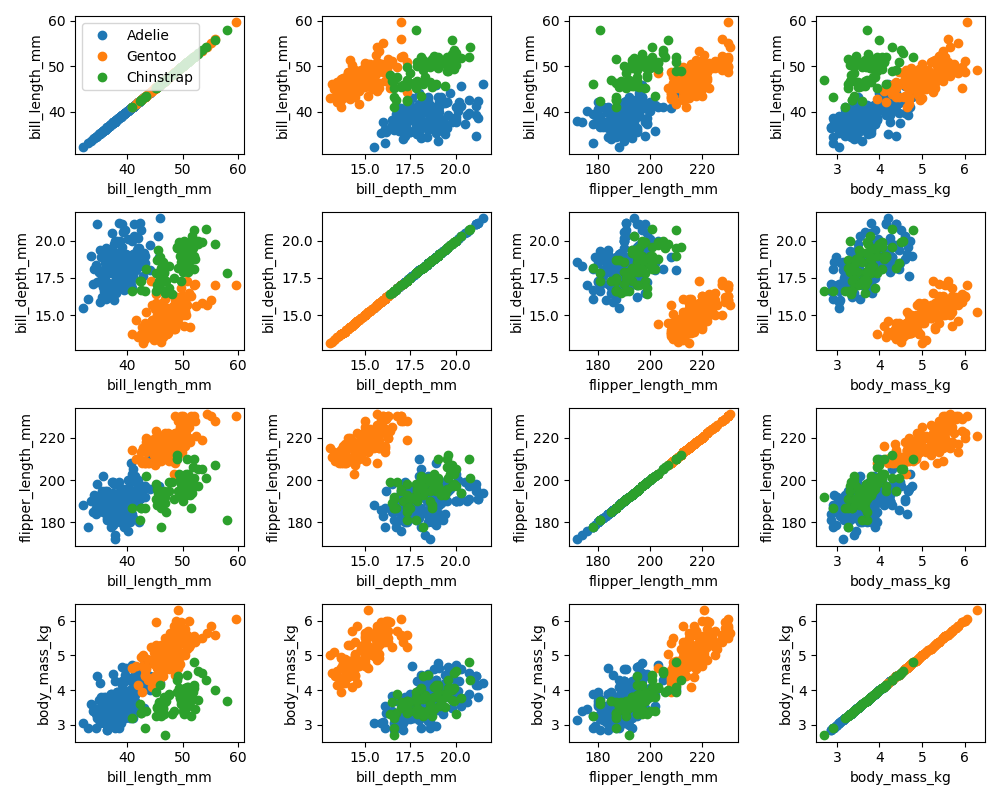
\includegraphics[width=0.75\textwidth,height=\textheight]{bilder/05-all-pairs.png}
\caption{Pinguin Datenset 2D plots}\label{fig:05-penguin-allpairs}
}
\end{figure}

Ein Blick auf die Diagonale zeigt schon, dass manche Merkmale besser geeignet als andere sind, um die Spezies zu unterscheiden. Allerdings reichen (in dieser linearen Darstellung) zwei Merkmale nicht aus, um eine eindeutige Diskriminierung zu erreichen.

\hypertarget{ein-2-layer-neuronales-netz-zur-klassifizierung}{%
\section{\texorpdfstring{Ein \emph{2}-Layer Neuronales Netz zur Klassifizierung}{Ein 2-Layer Neuronales Netz zur Klassifizierung}}\label{ein-2-layer-neuronales-netz-zur-klassifizierung}}

Wir definieren ein neuronales Netzes \(\mathcal N\) mit einer \emph{hidden layer} als
\begin{equation*}
\eta_i = \mathcal N (x_i):=\tanh \bigl (A_2 \tanh (A_1 x_i + b_1) + b_2\bigr ),
\end{equation*}
das für einen Datenpunkt \(x_i \in \mathbb R^{n_0}\) einen Ergebniswert \(\eta_i\in \mathbb R^{n_2}\) liefert.
Die sogenannten Gewichte \(A_1 \in \mathbb R^{n_1 \times n_0}\), \(b_1 \in \mathbb R^{n_1}\), \(A_2 \in \mathbb R^{n_2, n_1}\), \(b_2 \in \mathbb R^{n_2}\) parametrisieren diese Funktion. Eine Schicht besteht aus der einer affin-linearen Abbildung und einer \emph{Aktivierungsfunktion} die hier als \(\tanh\) gewählt wird und die komponentenweise angewendet wird.

Wir werden \(n_0=4\) (soviele Merkmale als Eingang) und \(n_2=1\) (eine
Entscheidungsvariable als Ausgang) setzen und das Netzwerk so trainieren, dass
anhand der gemessenen Daten \(x_i\) die bekannte Pinguin Population
\href{files/penguin-data.json}{\texttt{penguin-data.json}} in zwei Gruppen aufgeteilt
werden, wobei in der ersten Gruppe eine Spezies enthalten ist und in der anderen
die beiden anderen Spezies.

Dazu kann eine Funktion \(\ell \colon X \mapsto \{-1, 1\}\) definiert werden, die die bekannten Pinguine \(x_i\) aus dem Datensatz \(X\) ihrer Gruppe zuordnet. Dann können die Koeffizienten von \(\mathcal N\) über das Optimierungsproblem
\begin{equation*}
\frac{1}{|X|}\sum_{x_i \in X} \|\ell(x_i)-\mathcal N(x_i)\|^2 \to \min_{A_1, b_1, A_2, b_2}
\end{equation*}
mittels des \emph{stochastischen (batch) Gradientenabstiegs} bestimmt werden.

Zur Optimierung wird typischerweise ein Teil (z.B. 90\%) der Datenpunkte
verwendet über die mehrfach (in sogenannten \emph{epochs}) iteriert wird.

Danach kann mittels der verbliebenen Datenpunkte getestet werden, wie gut das
Netzwerk Daten interpretiert, die es noch nicht ``gesehen'' hat.

\hypertarget{beispiel-implementierung}{%
\section{Beispiel Implementierung}\label{beispiel-implementierung}}

Für ein 2-layer Netzwerk zur Klassifizierung der Pinguine.

Hier ein \href{files/051_sngltarg.py}{python file} oder ein \href{files/051_sngltarg.ipynb}{ipython
file} sowie die \href{files/penguin-data.json}{Pinguin
Daten} zum Direktdownload.

\hypertarget{setup}{%
\subsection{Setup}\label{setup}}

Wir importieren die benötigten Module und laden die Daten.

\begin{Shaded}
\begin{Highlighting}[]
\CommentTok{\# import the required modules}
\ImportTok{import}\NormalTok{ json}
\ImportTok{import}\NormalTok{ numpy }\ImportTok{as}\NormalTok{ np}
\ImportTok{import}\NormalTok{ matplotlib.pyplot }\ImportTok{as}\NormalTok{ plt}
\ImportTok{from}\NormalTok{ scipy.optimize }\ImportTok{import}\NormalTok{ approx\_fprime  }\CommentTok{\# we will use this function to compute gradients}

\CommentTok{\# load the data}
\ControlFlowTok{with} \BuiltInTok{open}\NormalTok{(}\StringTok{\textquotesingle{}penguin{-}data.json\textquotesingle{}}\NormalTok{, }\StringTok{\textquotesingle{}r\textquotesingle{}}\NormalTok{) }\ImportTok{as}\NormalTok{ f:}
\NormalTok{    datadict }\OperatorTok{=}\NormalTok{ json.load(f)}
\CommentTok{\# turn it into a numpy array}
\NormalTok{data }\OperatorTok{=}\NormalTok{ np.array(datadict[}\StringTok{\textquotesingle{}data\textquotesingle{}}\NormalTok{])}
\NormalTok{data }\OperatorTok{=}\NormalTok{ data }\OperatorTok{{-}}\NormalTok{ data.mean(axis}\OperatorTok{=}\DecValTok{0}\NormalTok{)  }\CommentTok{\# center the data}
\CommentTok{\# extract the labels}
\NormalTok{lbls }\OperatorTok{=}\NormalTok{ np.array(datadict[}\StringTok{\textquotesingle{}target\textquotesingle{}}\NormalTok{])}
\end{Highlighting}
\end{Shaded}

In diesem Beispiel unterscheiden wir nur zwei Gruppen. Wir teilen die
ersetzen die eigentlichen \emph{labels} \texttt{{[}0,\ 1,\ 2{]}} durch die zwei \emph{lables} \texttt{{[}-1,\ 1{]}}.

\begin{Shaded}
\begin{Highlighting}[]
\CommentTok{\# a dictionary that maps the labels(=targets) of the data into labels \{1, {-}1\}}
\CommentTok{\# that will use for distinction of two groups}
\NormalTok{mplbldict }\OperatorTok{=}\NormalTok{ \{}\DecValTok{0}\NormalTok{: np.array([}\DecValTok{1}\NormalTok{]),}
             \DecValTok{1}\NormalTok{: np.array([}\DecValTok{1}\NormalTok{]),}
             \DecValTok{2}\NormalTok{: np.array([}\OperatorTok{{-}}\DecValTok{1}\NormalTok{])\}}
\BuiltInTok{print}\NormalTok{(}\StringTok{\textquotesingle{}our two groups: }\CharTok{\textbackslash{}n}\StringTok{\textquotesingle{}}\NormalTok{, [}\SpecialStringTok{f\textquotesingle{}}\SpecialCharTok{\{}\NormalTok{datadict[}\StringTok{"target\_names"}\NormalTok{][lblid]}\SpecialCharTok{\}}\SpecialStringTok{ {-}{-}\textgreater{} }\SpecialCharTok{\{}\NormalTok{mplbldict[lblid]}\SpecialCharTok{.}\NormalTok{item()}\SpecialCharTok{\}}\SpecialStringTok{\textquotesingle{}} \ControlFlowTok{for}\NormalTok{ lblid }\KeywordTok{in}\NormalTok{ [}\DecValTok{0}\NormalTok{, }\DecValTok{1}\NormalTok{, }\DecValTok{2}\NormalTok{]])}
\end{Highlighting}
\end{Shaded}

Als nächstes legen wir die Dimensionen der \emph{layers} fest und damit auch die
Größe der Gewichtsmatrizen. Bei unserem 2-layer Netzwerk, bleibt uns
da nur die Größe der mittleren Schicht, da die Eingangsdimension
durch die Daten und die Ausgangsdimension durch unsere Wahl, wie wir entscheiden
wollen, bereits festgelegt ist.

\begin{Shaded}
\begin{Highlighting}[]
\CommentTok{\# sizes of the layers}
\NormalTok{sxz, sxo, sxt }\OperatorTok{=}\NormalTok{ data.shape[}\DecValTok{1}\NormalTok{], }\DecValTok{2}\NormalTok{, mplbldict[}\DecValTok{0}\NormalTok{].size}
\CommentTok{\# defines also the sizes of the weightmatrices}
\end{Highlighting}
\end{Shaded}

Zuletzt noch die Parameter, die das \emph{training} definieren.

\begin{itemize}
\tightlist
\item
  \texttt{batchsize} -- über wieviele Samples wird der stochastische Gradient
  bestimmt
\item
  \texttt{lr} -- \emph{learning rate} -- die Schrittweite
\item
  \texttt{epochs} -- wie oft wird über die Daten iteriert
\end{itemize}

und dann wie gross der Anteil und was die Indizes der Trainings--
beziehungsweise Testdaten sind

\begin{Shaded}
\begin{Highlighting}[]
\CommentTok{\# parameters for the training {-}{-} these worked fine for me}
\NormalTok{batchsize }\OperatorTok{=} \DecValTok{30}  \CommentTok{\# how many samples for the stochastic gradients}
\NormalTok{lr }\OperatorTok{=} \FloatTok{0.125}  \CommentTok{\# learning rate}
\NormalTok{epochs }\OperatorTok{=} \DecValTok{1000}  \CommentTok{\# how many gradient steps}

\CommentTok{\# the data}
\NormalTok{traindataratio }\OperatorTok{=} \FloatTok{.9}     \CommentTok{\# the ratio of training data vs. test data}
\NormalTok{ndata }\OperatorTok{=}\NormalTok{ data.shape[}\DecValTok{0}\NormalTok{]   }\CommentTok{\# number of datapoints                                       }
\NormalTok{trnds }\OperatorTok{=} \BuiltInTok{int}\NormalTok{(ndata}\OperatorTok{*}\NormalTok{traindataratio)}
\NormalTok{allidx }\OperatorTok{=}\NormalTok{ np.arange(ndata)                                   }\CommentTok{\# indices of all data}
\NormalTok{trnidx }\OperatorTok{=}\NormalTok{ np.random.choice(allidx, trnds, replace}\OperatorTok{=}\VariableTok{False}\NormalTok{)     }\CommentTok{\# training ids}
\NormalTok{tstidx }\OperatorTok{=}\NormalTok{ np.setdiff1d(allidx, trnidx)                       }\CommentTok{\# test ids}
\end{Highlighting}
\end{Shaded}

\hypertarget{neural-network-evaluation-setup}{%
\subsection{Neural Network Evaluation Setup}\label{neural-network-evaluation-setup}}

Hier definieren wir das Netzwerk als Funktion der Parameter und die \emph{loss function}, die misst wie gut das Netzwerk die Daten wiedergibt und die Grundlage fuer die Optimierung ist.

\begin{Shaded}
\begin{Highlighting}[]
\KeywordTok{def}\NormalTok{ fwdnn(xzero, Aone}\OperatorTok{=}\VariableTok{None}\NormalTok{, bone}\OperatorTok{=}\VariableTok{None}\NormalTok{, Atwo}\OperatorTok{=}\VariableTok{None}\NormalTok{, btwo}\OperatorTok{=}\VariableTok{None}\NormalTok{):}
    \CommentTok{\textquotesingle{}\textquotesingle{}\textquotesingle{} definition/(forward)evaluation of a neural networks of two layers}

\CommentTok{    \textquotesingle{}\textquotesingle{}\textquotesingle{}}
\NormalTok{    xone }\OperatorTok{=}\NormalTok{ np.tanh(Aone }\OperatorTok{@}\NormalTok{ xzero }\OperatorTok{+}\NormalTok{ bone)}
\NormalTok{    xtwo }\OperatorTok{=}\NormalTok{ np.tanh(Atwo }\OperatorTok{@}\NormalTok{ xone }\OperatorTok{+}\NormalTok{ btwo)}
    \ControlFlowTok{return}\NormalTok{ xtwo}
\end{Highlighting}
\end{Shaded}

\begin{Shaded}
\begin{Highlighting}[]
\KeywordTok{def}\NormalTok{ sqrdloss(weightsvector, features}\OperatorTok{=}\VariableTok{None}\NormalTok{, labels}\OperatorTok{=}\VariableTok{None}\NormalTok{):}
    \CommentTok{\textquotesingle{}\textquotesingle{}\textquotesingle{} compute the sqrd \textasciigrave{}loss\textasciigrave{}}

\CommentTok{    || NN(x\_i) {-} y\_i ||\^{}2}

\CommentTok{    given the vector of weights for a given data point (features)}
\CommentTok{    and the corresponding label}
\CommentTok{    \textquotesingle{}\textquotesingle{}\textquotesingle{}}

\NormalTok{    Aone, bone, Atwo, btwo }\OperatorTok{=}\NormalTok{ wvec\_to\_wmats(weightsvector)}
    \CommentTok{\# compute the prediction}
\NormalTok{    nnpred }\OperatorTok{=}\NormalTok{ fwdnn(features, Aone}\OperatorTok{=}\NormalTok{Aone, bone}\OperatorTok{=}\NormalTok{bone, Atwo}\OperatorTok{=}\NormalTok{Atwo, btwo}\OperatorTok{=}\NormalTok{btwo)}
    \ControlFlowTok{return}\NormalTok{ np.linalg.norm(nnpred }\OperatorTok{{-}}\NormalTok{ labels)}\OperatorTok{**}\DecValTok{2}
\end{Highlighting}
\end{Shaded}

An sich liegen die Parameter als Matrizen vor. Da jedoch die Theorie (und auch die praktische Implementierung) einen Parameter\textbf{vektor} voraussetzt, entrollen wir die Matrizen und stecken sie in einen grossen Vektor. Dann muessen wir noch an der richtigen Stelle wieder die Matrizen aus dem Vektor extrahieren; was die folgende Funktion realisiert.

\begin{Shaded}
\begin{Highlighting}[]
\KeywordTok{def}\NormalTok{ wvec\_to\_wmats(wvec):}
    \CommentTok{\textquotesingle{}\textquotesingle{}\textquotesingle{} helper to turn the vector of weights into the system matrices}

\CommentTok{    \textquotesingle{}\textquotesingle{}\textquotesingle{}}
\NormalTok{    Aone }\OperatorTok{=}\NormalTok{ wvec[:sxz}\OperatorTok{*}\NormalTok{sxo].reshape((sxo, sxz))}
\NormalTok{    cidx }\OperatorTok{=}\NormalTok{ sxz}\OperatorTok{*}\NormalTok{sxo}
\NormalTok{    bone }\OperatorTok{=}\NormalTok{ wvec[cidx:cidx}\OperatorTok{+}\NormalTok{sxo]}
\NormalTok{    cidx }\OperatorTok{=}\NormalTok{ cidx }\OperatorTok{+}\NormalTok{ sxo}
\NormalTok{    Atwo }\OperatorTok{=}\NormalTok{ wvec[cidx:cidx}\OperatorTok{+}\NormalTok{sxo}\OperatorTok{*}\NormalTok{sxt].reshape((sxt, sxo))}
\NormalTok{    cidx }\OperatorTok{=}\NormalTok{ cidx }\OperatorTok{+}\NormalTok{ sxo}\OperatorTok{*}\NormalTok{sxt}
\NormalTok{    btwo }\OperatorTok{=}\NormalTok{ wvec[cidx:]}
    \ControlFlowTok{if}\NormalTok{ Aone.size }\OperatorTok{+}\NormalTok{ bone.size }\OperatorTok{+}\NormalTok{ Atwo.size }\OperatorTok{+}\NormalTok{ btwo.size }\OperatorTok{==}\NormalTok{ wvec.size:}
        \ControlFlowTok{return}\NormalTok{ Aone, bone, Atwo, btwo}
    \ControlFlowTok{else}\NormalTok{:}
        \ControlFlowTok{raise} \PreprocessorTok{UserWarning}\NormalTok{(}\StringTok{\textquotesingle{}mismatch weightsvector/matrices\textquotesingle{}}\NormalTok{)}
\end{Highlighting}
\end{Shaded}

\hypertarget{das-training}{%
\subsection{Das Training}\label{das-training}}

Der Parametervektor (``die Gewichte'') werden zufällig initialisiert und dann mit dem stochastischen Gradienten in mehreren Epochen optimiert.

\textbf{Bemerkung}: Hier benutzen wir \texttt{scipy.optimize.approx\_fprime} um den
Gradienten numerisch zu bestimmen. Das ist hochgradig ineffizient. ``Richtige''
Implementierungen von \emph{Machine Learning} Bibliotheken benutzen anstelle
\emph{Automatisches Differenzieren} für eine sowohl schnelle und als auch akkurate Berechnung des Gradienten.

\begin{Shaded}
\begin{Highlighting}[]
\CommentTok{\# initialization of the weights}
\NormalTok{wini }\OperatorTok{=}\NormalTok{ np.random.randn(sxo}\OperatorTok{*}\NormalTok{sxz }\OperatorTok{+}\NormalTok{ sxo }\OperatorTok{+}\NormalTok{ sxt}\OperatorTok{*}\NormalTok{sxo }\OperatorTok{+}\NormalTok{ sxt)}
\NormalTok{gradnrml }\OperatorTok{=}\NormalTok{ []  }\CommentTok{\# list of norm of grads for plotting later}

\NormalTok{cwghts }\OperatorTok{=}\NormalTok{ wini  }\CommentTok{\# the current state of the weight vector}
\ControlFlowTok{for}\NormalTok{ kkk }\KeywordTok{in} \BuiltInTok{range}\NormalTok{(epochs):}
\NormalTok{    cids }\OperatorTok{=}\NormalTok{ np.random.choice(trnidx, batchsize, replace}\OperatorTok{=}\VariableTok{False}\NormalTok{)}
\NormalTok{    cgrad }\OperatorTok{=}\NormalTok{ np.zeros(wini.shape)}
    \ControlFlowTok{for}\NormalTok{ cid }\KeywordTok{in}\NormalTok{ cids:}
\NormalTok{        itrgts }\OperatorTok{=}\NormalTok{ data[cid, :]}
\NormalTok{        ilabls }\OperatorTok{=}\NormalTok{ mplbldict[lbls[cid]]}
\NormalTok{        cgrad }\OperatorTok{=}\NormalTok{ cgrad }\OperatorTok{+}\NormalTok{ approx\_fprime(cwghts, sqrdloss, }\FloatTok{1e{-}8}\NormalTok{,}
\NormalTok{                                      itrgts, ilabls)}
\NormalTok{    cwghts }\OperatorTok{=}\NormalTok{ cwghts }\OperatorTok{{-}}\NormalTok{ lr}\OperatorTok{*}\DecValTok{1}\OperatorTok{/}\NormalTok{batchsize}\OperatorTok{*}\NormalTok{cgrad  }\CommentTok{\# the upgrade}
\NormalTok{    gradnrml.append(}\DecValTok{1}\OperatorTok{/}\NormalTok{batchsize}\OperatorTok{*}\NormalTok{np.linalg.norm(cgrad))}
    \ControlFlowTok{if}\NormalTok{ np.mod(kkk, }\DecValTok{50}\NormalTok{) }\OperatorTok{==} \DecValTok{0}\NormalTok{:}
        \BuiltInTok{print}\NormalTok{(}\SpecialStringTok{f\textquotesingle{}k=}\SpecialCharTok{\{}\NormalTok{kkk}\SpecialCharTok{\}}\SpecialStringTok{: norm of gradient: }\SpecialCharTok{\{np.}\NormalTok{linalg}\SpecialCharTok{.}\NormalTok{norm(cgrad)}\SpecialCharTok{\}}\SpecialStringTok{\textquotesingle{}}\NormalTok{)}
\end{Highlighting}
\end{Shaded}

\begin{Shaded}
\begin{Highlighting}[]
\NormalTok{plt.figure()}
\NormalTok{plt.semilogy(gradnrml, label}\OperatorTok{=}\StringTok{\textquotesingle{}norm of gradient estimate\textquotesingle{}}\NormalTok{)}
\NormalTok{plt.xlabel(}\StringTok{\textquotesingle{}$k${-}th stochastic gradient step\textquotesingle{}}\NormalTok{)}
\NormalTok{plt.legend()}
\NormalTok{plt.show()}
\end{Highlighting}
\end{Shaded}

\begin{figure}
\centering
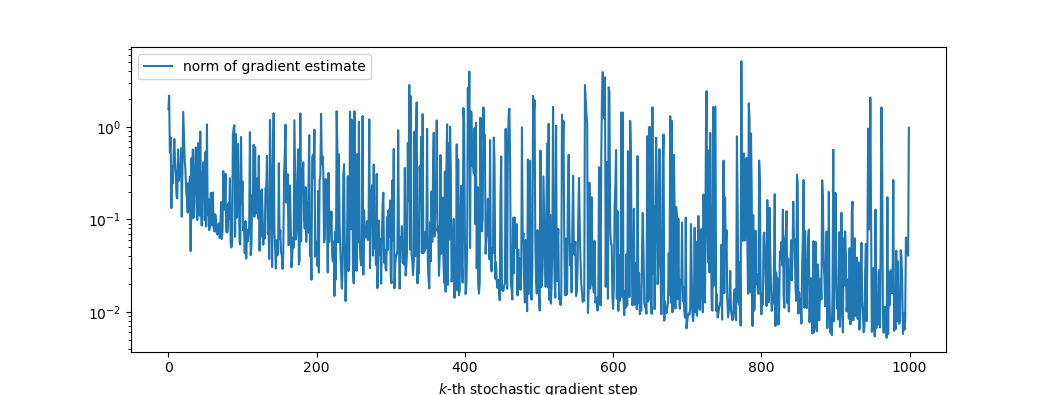
\includegraphics{bilder/051_nnpeng_conv.png}
\caption{Beispiel Konvergenz des Stochastischen Gradienten}
\end{figure}

Wir koennen eine gewisse Konvergenz beobachten (sichtbar an der unteren Kante) aber auch ein typisches stochastisches Verhalten.

\hypertarget{das-auswerten}{%
\subsection{Das Auswerten}\label{das-auswerten}}

Wir nehmen das Ergebnis der letzten Iteration als \emph{beste Parameter}, definieren damit das Neuronale Netz, und testen auf den übriggebliebenen Daten das Ergebnis.

\begin{Shaded}
\begin{Highlighting}[]
\NormalTok{optwghts }\OperatorTok{=}\NormalTok{ cwghts  }\CommentTok{\# the optimal weights}
\NormalTok{Aonex, bonex, Atwox, btwox }\OperatorTok{=}\NormalTok{ wvec\_to\_wmats(optwghts)}
\end{Highlighting}
\end{Shaded}

\begin{Shaded}
\begin{Highlighting}[]
\BuiltInTok{print}\NormalTok{(}\StringTok{\textquotesingle{}***** testing the classification *****\textquotesingle{}}\NormalTok{)}
\NormalTok{faillst }\OperatorTok{=}\NormalTok{ []}
\ControlFlowTok{for}\NormalTok{ cti }\KeywordTok{in}\NormalTok{ tstidx:  }\CommentTok{\# iteration over the test data points}
\NormalTok{    itrgt }\OperatorTok{=}\NormalTok{ data[cti, :]}
\NormalTok{    ilbl }\OperatorTok{=}\NormalTok{ mplbldict[lbls[cti]]}
    \CommentTok{\# the prediction of the neural network}
\NormalTok{    nnlbl }\OperatorTok{=}\NormalTok{ fwdnn(itrgt, Aone}\OperatorTok{=}\NormalTok{Aonex, bone}\OperatorTok{=}\NormalTok{bonex, Atwo}\OperatorTok{=}\NormalTok{Atwox, btwo}\OperatorTok{=}\NormalTok{btwox)}
\NormalTok{    sccs }\OperatorTok{=}\NormalTok{ np.sign(ilbl) }\OperatorTok{==}\NormalTok{ np.sign(nnlbl)}
    \BuiltInTok{print}\NormalTok{(}\SpecialStringTok{f\textquotesingle{}label: }\SpecialCharTok{\{}\NormalTok{ilbl}\SpecialCharTok{.}\NormalTok{item()}\SpecialCharTok{\}}\SpecialStringTok{ {-}{-} nn: }\SpecialCharTok{\{}\NormalTok{nnlbl}\SpecialCharTok{.}\NormalTok{item()}\SpecialCharTok{:.4f\}}\SpecialStringTok{ {-}{-} success: }\SpecialCharTok{\{}\NormalTok{sccs}\SpecialCharTok{\}}\SpecialStringTok{\textquotesingle{}}\NormalTok{)}
    \ControlFlowTok{if} \KeywordTok{not}\NormalTok{ sccs:}
\NormalTok{        faillst.append((cti, ilbl.item(), nnlbl.item(),}
\NormalTok{                        datadict[}\StringTok{\textquotesingle{}target\_names\textquotesingle{}}\NormalTok{][lbls[cti]]))}
    \ControlFlowTok{else}\NormalTok{:}
        \ControlFlowTok{pass}
\end{Highlighting}
\end{Shaded}

\begin{Shaded}
\begin{Highlighting}[]
\BuiltInTok{print}\NormalTok{(}\StringTok{\textquotesingle{}}\CharTok{\textbackslash{}n}\StringTok{***** Results *****\textquotesingle{}}\NormalTok{)}
\BuiltInTok{print}\NormalTok{(}\SpecialStringTok{f\textquotesingle{}}\SpecialCharTok{\{}\DecValTok{100}\OperatorTok{{-}}\BuiltInTok{len}\NormalTok{(faillst)}\OperatorTok{/}\NormalTok{tstidx}\SpecialCharTok{.}\NormalTok{size}\OperatorTok{*}\DecValTok{100}\SpecialCharTok{:.0f\}}\SpecialStringTok{\% was classified correctly\textquotesingle{}}\NormalTok{)}
\BuiltInTok{print}\NormalTok{(}\StringTok{\textquotesingle{}***** Misses *****\textquotesingle{}}\NormalTok{)}
\ControlFlowTok{if} \BuiltInTok{len}\NormalTok{(faillst) }\OperatorTok{==} \DecValTok{0}\NormalTok{:}
    \BuiltInTok{print}\NormalTok{(}\StringTok{\textquotesingle{}None\textquotesingle{}}\NormalTok{)}
\ControlFlowTok{else}\NormalTok{:}
    \ControlFlowTok{for}\NormalTok{ cfl }\KeywordTok{in}\NormalTok{ faillst:}
\NormalTok{        cid, lbl, nnlbl, name }\OperatorTok{=}\NormalTok{ cfl}
        \BuiltInTok{print}\NormalTok{(}\SpecialStringTok{f\textquotesingle{}ID: }\SpecialCharTok{\{}\NormalTok{cid}\SpecialCharTok{\}}\SpecialStringTok{ (}\SpecialCharTok{\{}\NormalTok{name}\SpecialCharTok{\}}\SpecialStringTok{ pinguin) was missclassified \textquotesingle{}} \OperatorTok{+}
              \SpecialStringTok{f\textquotesingle{}with score }\SpecialCharTok{\{}\NormalTok{nnlbl}\SpecialCharTok{:.4f\}}\SpecialStringTok{ vs. }\SpecialCharTok{\{}\NormalTok{lbl}\SpecialCharTok{\}}\SpecialStringTok{\textquotesingle{}}\NormalTok{)}
\end{Highlighting}
\end{Shaded}

\hypertarget{singuluxe4rwert-zerlegung}{%
\chapter{Singulärwert Zerlegung}\label{singuluxe4rwert-zerlegung}}

Die Singulärwertzerlegung ist ein Universalwerkzeug der Datenanalyse und
Modellsynthese.
Die wesentliche Eigenschaft ist die Quantifizierung
wesentlicher und redundanter Anteile in Daten oder Operatoren.

Die direkte Anwendung ist die \emph{Principal Component Analysis}, die orthogonale Dimensionen in multivariablen Daten identifiziert, die nach der Stärke der Varianz sortiert sind. So kann diese erste \emph{principal component} als die \emph{reichhaltigste} Datenrichtung interpretiert werden und die letzten Richtungen (insbesondere wenn die Varianz komplett verschwindet) als wenig aussagekräftig (und insbesondere redundant) identifiziert werden.

Andere Anwendungen ist die Lösung von überbestimmten
Gleichungssystemen (wie sie in der linearen Regression vorkommen) oder das
Entfernen von \emph{Rauschen} aus Daten.

\hypertarget{definition-und-eigenschaften}{%
\section{Definition und Eigenschaften}\label{definition-und-eigenschaften}}

\begin{theorem}[Singulärwertzerlegung (SVD)]
\protect\hypertarget{thm:SVD}{}\label{thm:SVD}Sei \(A\in \mathbb C^{m\times n}\), \(m\geq n\). Dann existieren orthogonale Matrizen \(U \in \mathbb C^{m\times m}\) und \(V\in \mathbb C^{n\times n}\) und eine Matrix \(\Sigma \in \mathbb R^{m\times n}\) der Form
\begin{equation*}
\Sigma = 
\begin{bmatrix}
\sigma_1 & 0 & \dots & 0\\
0 & \sigma_2 &\ddots & \vdots\\
0 & \ddots & \ddots &0\\
  0 & \dots&0 & \sigma_n \\
  0 & 0 & \dots & 0 \\
  \vdots & \ddots &  & \vdots\\
  0 & 0 & \dots & 0
\end{bmatrix}
\end{equation*}
mit reellen sogenannten \emph{Singulärwerten}
\begin{equation*}
\sigma_1 \geq \sigma_2 \geq \dots \geq \sigma_n \geq 0
\end{equation*}
sodass gilt
\begin{equation*}
A = U \Sigma V^*
\end{equation*}
wobei gilt \(V^* = \overline{V^T}\) (transponiert und komplex konjugiert).
\end{theorem}

Ein paar Bemerkungen.

\begin{itemize}
\tightlist
\item
  Ist \(A\) reell, können auch \(U\) und \(V\) reell gewählt werden.
\item
  Ein Beweis ist in (Bollhöfer and Mehrmann \protect\hyperlink{ref-BolM04}{2004}, Satz 14.14) zu finden.
\item
  Die Annahme \(m \geq n\) war nur nötig um für die Matrix \(\Sigma\) keine Fallunterscheidung zu machen. (Für \(m\leq n\) ``steht der Nullblock rechts von den Singulärwerten''). Insbesondere gilt \(A^* = V\Sigma U^*\) ist eine SVD von \(A^*\).
\item
  Eine Illustration der Zerlegung ist Abbildung \ref{fig:fig-SVD} zu sehen.
\end{itemize}

Wir machen einige Überlegungen im Hinblick auf große Matrizen. Sei dazu \(m>n\), \(A\in \mathbb C^{m\times n}\) und \(A=U\Sigma V^*\) eine SVD wie in Theorem \ref{thm:SVD}. Sei nun
\begin{equation*}
U = \begin{bmatrix}
U_1 & U_2
\end{bmatrix}
% = \begin{bmatrix} V_1^* & V_2^*
\end{equation*}
partitioniert sodass \(U_1\) die ersten \(n\) Spalten von \(U\) enthält.

Dann gilt (nach der Matrix-Multiplikations Regel \emph{Zeile mal Spalte} die Teile \(U_2\) und \(V_2\) immer mit dem Nullblock in \(\Sigma\) multipliziert werden) dass
\begin{equation*}
A = U\Sigma V = 
\begin{bmatrix}
U_1 & U_2
\end{bmatrix}
\begin{bmatrix}
\hat \Sigma \\ 0
\end{bmatrix}
V^*
% \begin{bmatrix} V_1^* \\ V_2^* \end{bmatrix}
=
U_1 
\hat \Sigma
V^*
% \begin{bmatrix} V_1^* \\ V_2^* \end{bmatrix}
\end{equation*}
Es genügt also nur die ersten \(m\) Spalten von \(U\) zu berechnen. Das ist die sogenannte \textbf{slim SVD}.

Hat, darüberhinaus, die Matrix \(A\) keinen vollen Rang, also \(\operatorname{Rg}(A) = r < n\), dann:

\begin{itemize}
\tightlist
\item
  ist \(\sigma_i=0\), für alle \(i=r+1, \dotsc, n\), (wir erinnern uns, dass die Singulärwerte nach Größe sortiert sind)
\item
  die Matrix \(\hat \Sigma\) hat \(n-r\) Nullzeilen
\item
  für die Zerlegung sind nur die ersten \(r\) Spalten von \(U\) und \(V\) relevant -- die sogenannte \textbf{Kompakte SVD}.
\end{itemize}

In der Datenapproximation ist außerdem die \textbf{truncated SVD} von Interesse. Dazu sei \(\hat r<r\) ein beliebig gewählter Index. Dann werden alle Singulärwerte, \(\sigma_i=0\), für alle \(i=\hat r+1, \dotsc, n\), abgeschnitten -- das heißt null gesetzt und die entsprechende \emph{kompakte SVD} berechnet.

Hier gilt nun nicht mehr die Gleichheit in der Zerlegung. Vielmehr gilt
\begin{equation*}
A \approx A_{\hat r}
\end{equation*}
wobei \(A_{\hat r}\) aus der \emph{truncated SVD} von \(A\) erzeugt wurde. Allerdings ist diese Approximation von \(A\) durch optimal in dem Sinne, dass es keine Matrix vom Rang \(\hat r \geq r=\operatorname{Rg}(A)\) gibt, die \(A\) (in der \emph{induzierten} euklidischen Norm) besser approximiert. Es gilt
\begin{equation*}
\min_{B\in \mathbb C^{m\times n}, \operatorname{Rg}(B)=\hat r} \|A-B\|_2 = \|A-A_{\hat r}\|_2 = \sigma_{\hat r + 1};
\end{equation*}
(vgl. Satz 14.15, Bollhöfer and Mehrmann \protect\hyperlink{ref-BolM04}{2004}).

Zum Abschluss noch der Zusammenhang zur \emph{linearen Ausgleichsrechnung}.
Die Lösung \(w\) des Problems der \emph{linearen Ausgleichsrechnung} war entweder als Lösung eines Optimierungsproblems
\begin{equation*}
\min_{w} \| Aw - y \|^2
\end{equation*}
oder als Lösung des linearen Gleichungssystems
\begin{equation*}
A^TAw=y.
\end{equation*}
Ist \(A=U\Sigma V^*=U_1\hat \Sigma V^*\) (slim) ``SV-zerlegt'', dann gilt
\begin{equation*}
A^*Aw = V\hat \Sigma^*U_1^*U_1\hat \Sigma V^*w = V\hat \Sigma^2 V^* w
\end{equation*}
und damit
\begin{equation*}
A^*Aw = A^*y \quad \Leftrightarrow \quad V\hat \Sigma^2 V^*w  = V\hat \Sigma^*U_1^*y \quad \Leftrightarrow \quad w = V\hat \Sigma^{-1} U_1^*y
\end{equation*}
was wir (mit den Matrizen der vollen SVD) als
\begin{equation*}
w = V \Sigma^+ U^*y
\end{equation*}
schreiben, wobei
\begin{equation*}
\Sigma^+ = \begin{bmatrix}
\hat \Sigma^{-1} \\ 0_{m-n \times n}
\end{bmatrix}
\end{equation*}
.

\textbf{Bemerkung}: \(\Sigma^+\) kann auch definiert werden, wenn \(\hat \Sigma\) nicht invertierbar ist (weil manche Diagonaleinträge null sind). Dann wird \(\hat \Sigma^+\) betrachtet, bei welcher nur die \(\sigma_i>0\) invertiert werden und die anderen \(\sigma_i=0\) belassen werden. Das definiert eine sogenannte \emph{verallgemeinerte Inverse} und löst auch das Optimierungsproblem falls \(A\) keinen vollen Rang hat.

\begin{figure}
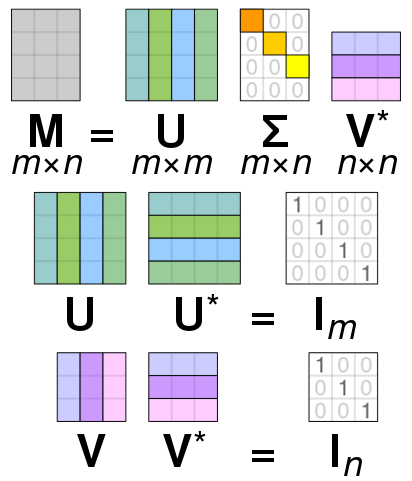
\includegraphics[width=0.5\linewidth]{bilder/06_412px-Singular_value_decomposition_visualisation.svg} \caption{Illustration der SVD. Bitte beachten, der $*$ bedeutet hier transponiert und komplex konjugiert. By Cmglee - Own work, CC BY-SA 4.0, https://commons.wikimedia.org/w/index.php?curid=67853297}\label{fig:fig-SVD}
\end{figure}

\hypertarget{numerische-berechnung}{%
\section{Numerische Berechnung}\label{numerische-berechnung}}

Die praktische Berechnung der Singulärwertzerlegung einer Matrix \(A\in \mathbb R^{m\times n}\) verlangt einen gesamten Grundkurs in \emph{numerischer
Mathematik}.

In direkter Weise könnten die Singulärwerte und --vektoren über
das Eigenwertproblem für \(AA^T\) oder \(A^TA\) bestimmt werden.
Das ist nicht so schlecht, wie mit dem Argument, \emph{dass sich mit dem
quadrieren der Matrizen auch die Konditionszahl quadriert}, gerne nahegelegt wird,\footnote{denn die Kondition des Eigenwertproblems ist direkt proportional zur Kondition der Matrix; vgl.
  (Satz 5.9, Richter and Wick \protect\hyperlink{ref-RicW17}{2017})} da

\begin{itemize}
\tightlist
\item
  wenn \(n\ll m\) oder \(m\ll n\), dann ist \(A^TA\) oder \(AA^T\) wesentlich kleiner
  als \(A\)
\item
  das Eigenwertproblem symmetrisch ist, was gut ausgenutzt werden kann
\item
  wenn \(A\) sehr gross aber \emph{dünnbesetzt} (engl. \emph{sparse}) ist, dann können die
  Eigenwerte durch effiziente \emph{sparse matrix-vector} Multiplikationen
  angenähert werden
\item
  es können ohne weiteres nur eine Anzahl von Singulärwerten
  berechnet werden
\end{itemize}

sodass für \emph{sparse} Matrizen diese Methode der de-facto Standard ist\footnote{und
  beispielsweise die Methode, die in
  \href{https://docs.scipy.org/doc/scipy/reference/generated/scipy.sparse.linalg.svds.html}{\texttt{scipy.sparse.linalg.svd}}
  implementiert ist}.

Für normale Matrizen kommt jedoch der folgende Algorithmus, der mehrere
wunderbar effiziente Algorithmen elegant kombiniert besser in Betracht:

\begin{enumerate}
\def\labelenumi{\arabic{enumi}.}
\tightlist
\item
  Betrachte
  \[M=\begin{bmatrix} 0 & A \\ A^T & 0 \end{bmatrix} \in \mathbb R^{n+m \times n+m},\]
  deren positiven Eigenwerte mit
  den (positiven) Singulärwerten von \(A\) übereinstimmen.
\item
  Bringe \(M\) durch \emph{Householder transformationen} in \emph{Hessenberg}-Form, also
  \[ H = QMQ^T \]
  mit \(Q\) orthogonal. Wegen Orthogonalität ist das eine
  Ähnlichkeitstransformation (\(H\) hat die gleichen Eigenwerte wie \(M\)) und
  wegen Symmetrie von \(M\) ist auch \(H\) symmetrisch und damit \emph{tridiagonal}.
\item
  Berechne die positiven Eigenwerte von \(H\) mittels der \emph{QR-Iteration}, die
  für \emph{Hessenbergmatrizen} sehr effizient implementiert werden kann.
\end{enumerate}

\textbf{Der Standard}\footnote{z.B. die
  \href{https://www.netlib.org/lapack/lug/node53.html\#3465}{LAPACK routinen}, die die Basis bspw. von \href{https://numpy.org/doc/stable/reference/generated/numpy.linalg.svd.html}{\texttt{numpy.linalg.svd}} aber auch von
  Matlab's SVD ist} funktioniert wie folgt:

\begin{enumerate}
\def\labelenumi{\arabic{enumi}.}
\tightlist
\item
  Berechne eine orthogonale Transformation auf eine \emph{bidiagonale}
  \(B=U_A^TAV_A\).
\item
  Berechne eine SVD von \(B=U_B\Sigma V_B^T\) (das wird effizient mit einem
  \href{https://dl.acm.org/doi/10.1137/S0895479892241287}{\emph{divide and conquer} Algorithmus von Gu und Eisenstat} getan)
\item
  Erhalte die gesuchte SVD als \(A=(U_AU_B)\Sigma (V_AV_B)^T\).
\end{enumerate}

\hypertarget{aufgaben}{%
\section{Aufgaben}\label{aufgaben}}

\hypertarget{norm-und-orthogonale-transformation}{%
\subsection{Norm und Orthogonale Transformation}\label{norm-und-orthogonale-transformation}}

Sei \(Q\in \mathbb R^{n\times n}\) eine orthogonale Matrix und sei \(y\in \mathbb R^{n}\). Zeigen Sie, dass
\begin{equation*}
\|y\|^2 = \|Qy \|^2
\end{equation*}
gilt.

\hypertarget{kleinste-quadrate-und-mittelwert}{%
\subsection{Kleinste Quadrate und Mittelwert}\label{kleinste-quadrate-und-mittelwert}}

Zeigen sie, dass der \emph{kleinste Quadrate} Ansatz zur Approximation einer Datenwolke
\begin{equation*}
(x_i, y_i), \quad i=1,2,\dotsc,N,
\end{equation*}
mittels einer konstanten Funktion \(f(x)=w_1\) auf \(w_1\) auf den Mittelwert der \(y_i\) führt.

\hypertarget{qr-zerlegung-und-kleinstes-quadrate-problem}{%
\subsection{QR Zerlegung und Kleinstes Quadrate Problem}\label{qr-zerlegung-und-kleinstes-quadrate-problem}}

Sei \(A\in \mathbb R^{m,n}\), \(m>n\), \(A\) hat vollen Rank und sei
\begin{equation*}
\begin{bmatrix}
Q_1 & Q_2
\end{bmatrix}
\begin{bmatrix}
\hat R \\ 0
\end{bmatrix} = A
\end{equation*}
eine QR-Zerlegung von \(A\) (d.h., dass \(Q\) unitär ist und \(\hat R\) eine (im
Falle, dass \(A\) vollen Rang hat invertierbare) obere Dreiecksmatrix. Zeigen sie, dass die Lösung von
\begin{equation*}
\hat R w = Q_1^T y
\end{equation*}
ein kritischer Punkt (d.h. der Gradient \(\nabla_w\) verschwindet) von
\begin{equation*}
w \mapsto \frac 12 \| Aw - y \|^2
\end{equation*}
ist, also \(w=\hat R^{-1}Q_1^T y\) eine Lösung des Optimierungsproblems
darstellt. Vergleichen Sie mit der SVD Lösung aus der Vorlesung.

\hypertarget{eigenwerte-symmetrischer-matrizen}{%
\subsection{Eigenwerte Symmetrischer Matrizen}\label{eigenwerte-symmetrischer-matrizen}}

Zeigen Sie, dass Eigenwerte symmetrischer reeller Matrizen \(A\in \mathbb R^{n\times n}\) immer reell sind.

\hypertarget{singuluxe4rwertzerlegung-und-eigenwerte-i}{%
\subsection{Singulärwertzerlegung und Eigenwerte I}\label{singuluxe4rwertzerlegung-und-eigenwerte-i}}

Zeigen Sie, dass die quadrierten Singulärwerte einer Matrix \(A\in \mathbb R^{m\times n}\), \(m>n\), genau die Eigenwerte der Matrix \(A^TA\) sind und beschreiben Sie in welcher Beziehung sie mit den Eigenwerten von \(AA^T\) stehen. \textbf{Hinweis}: hier ist ``\(m>n\)'' wichtig.

\hypertarget{singuluxe4rwertzerlegung-und-eigenwerte-ii}{%
\subsection{Singulärwertzerlegung und Eigenwerte II}\label{singuluxe4rwertzerlegung-und-eigenwerte-ii}}

Weisen Sie nach, dass die positiven Eigenwerte von
\begin{equation*}
\begin{bmatrix}
0 & A^T \\ A & 0
\end{bmatrix}
\end{equation*}
genau die \emph{nicht-null} Singulärwerte von \(A\) sind.

\hypertarget{truncated-svd}{%
\subsection{Truncated SVD}\label{truncated-svd}}

\begin{enumerate}
\def\labelenumi{\arabic{enumi}.}
\tightlist
\item
  Berechnen und plotten sie die Singulärwerte einer \(4000\times 1000\) Matrix mit zufälligen Einträgen und die einer Matrix mit ``echten'' Daten (hier Simulationsdaten einer Stroemungssimulation)\footnote{ \href{https://cloud.tu-ilmenau.de/s/pAMyTmK5YA5t9dg}{Download bitte hier} -- Achtung das sind 370MB}. Berechnen sie den Fehler der \emph{truncated SVD} \(\|A-A_{\hat r}\|\) für \(\hat r = 10, 20, 40\) für beide Matrizen.
\item
  Was lässt sich bezüglich einer Kompression der Daten mittels SVD für die beiden Matrizen sagen. (Vergleichen sie die plots der Singulärwerte und beziehen sie sich auf die gegebene Formel für die Differenz).
\item
  Für die ``echten'' Daten: Speichern sie die Faktoren der bei \(\hat r=40\) abgeschnittenen SVD und vergleichen Sie den Speicherbedarf der Faktoren und der eigentlichen Matrix.
\end{enumerate}

Beispielcode:

\begin{Shaded}
\begin{Highlighting}[]
\ImportTok{import}\NormalTok{ numpy }\ImportTok{as}\NormalTok{ np}
\ImportTok{import}\NormalTok{ scipy.linalg }\ImportTok{as}\NormalTok{ spla}
\ImportTok{import}\NormalTok{ matplotlib.pyplot }\ImportTok{as}\NormalTok{ plt}

\NormalTok{randmat }\OperatorTok{=}\NormalTok{ np.random.randn(}\DecValTok{4000}\NormalTok{, }\DecValTok{1000}\NormalTok{)}

\NormalTok{rndU, rndS, rndV }\OperatorTok{=}\NormalTok{ spla.svd(randmat)}

\BuiltInTok{print}\NormalTok{(}\StringTok{\textquotesingle{}U{-}dims: \textquotesingle{}}\NormalTok{, rndU.shape)}
\BuiltInTok{print}\NormalTok{(}\StringTok{\textquotesingle{}V{-}dims: \textquotesingle{}}\NormalTok{, rndV.shape)}
\BuiltInTok{print}\NormalTok{(}\StringTok{\textquotesingle{}S{-}dims: \textquotesingle{}}\NormalTok{, rndS.shape)}

\NormalTok{plt.figure(}\DecValTok{1}\NormalTok{)}
\NormalTok{plt.semilogy(rndS, }\StringTok{\textquotesingle{}.\textquotesingle{}}\NormalTok{, label}\OperatorTok{=}\StringTok{\textquotesingle{}Singulaerwerte (random Matrix)\textquotesingle{}}\NormalTok{)}

\NormalTok{realdatamat }\OperatorTok{=}\NormalTok{ np.load(}\StringTok{\textquotesingle{}velfielddata.npy\textquotesingle{}}\NormalTok{)}

\CommentTok{\# \# Das hier ist eine aufwaendige Operation}
\NormalTok{rlU, rlS, rlV }\OperatorTok{=}\NormalTok{ spla.svd(realdatamat, full\_matrices}\OperatorTok{=}\VariableTok{False}\NormalTok{)}
\CommentTok{\# \# auf keinen Fall \textasciigrave{}full\_matrices=False\textasciigrave{} vergessen}

\BuiltInTok{print}\NormalTok{(}\StringTok{\textquotesingle{}U{-}dims: \textquotesingle{}}\NormalTok{, rlU.shape)}
\BuiltInTok{print}\NormalTok{(}\StringTok{\textquotesingle{}V{-}dims: \textquotesingle{}}\NormalTok{, rlV.shape)}
\BuiltInTok{print}\NormalTok{(}\StringTok{\textquotesingle{}S{-}dims: \textquotesingle{}}\NormalTok{, rlS.shape)}

\NormalTok{plt.figure(}\DecValTok{1}\NormalTok{)}
\NormalTok{plt.semilogy(rlS, }\StringTok{\textquotesingle{}.\textquotesingle{}}\NormalTok{, label}\OperatorTok{=}\StringTok{\textquotesingle{}Singulaerwerte (Daten Matrix)\textquotesingle{}}\NormalTok{)}

\NormalTok{plt.legend()}
\NormalTok{plt.show()}
\end{Highlighting}
\end{Shaded}

\textbf{Hinweis}: Es gibt viele verschiedene Normen für Vektoren und Matrizen. Sie dürfen einfach mit \texttt{np.linalg.norm} arbeiten. Gerne aber mal in die Dokumentation schauen \emph{welche} Norm berechnet wird.

\hypertarget{pca-und-weitere-svd-anwendungen}{%
\chapter{PCA und weitere SVD Anwendungen}\label{pca-und-weitere-svd-anwendungen}}

\hypertarget{proper-orthogonal-decomposition-pod}{%
\section{Proper-Orthogonal Decomposition -- POD}\label{proper-orthogonal-decomposition-pod}}

Die POD Methode ist ein Ansatz um den hohen Rechen-- und Speicheraufwand in der
Simulation von hochdimensionalen (d.h. viele Variable umfassenden) Simulationen
von dynamischen Systemen abzumildern.
Grob gesagt funktioniert POD wie folgt.

Es sei ein dynamisches System
\begin{equation*}
\dot y(t) = f(t, y(t)), \quad y(0)=y_0 \in \mathbb R^{m}
\end{equation*}
gegeben, das die Entwicklung eines Zustandes \(y(t)\in \mathbb R^{m}\) über
die Zeit \(t>0\) beschreibt. Je größer die Dimension \(m\) ist, desto
aufwändiger ist das numerische berechnen (bzw. approximieren) der Werte von \(y\).

Die Idee von POD ist

\begin{enumerate}
\def\labelenumi{\arabic{enumi}.}
\item
  anzunehmen, dass die Zustände \(y(t)\) mit weniger
  als \(m\) Koordinaten beschrieben werden können, also
  \begin{equation*}
  y(t) \approx V\hat y(t)
  \end{equation*}
  mit einer Basismatrix \(U_r\in \mathbb R^{m\times r}\), \(r\leq m\), und reduzierten
  Koordinaten \(\hat y(t)\in \mathbb R^{r}\)
\item
  die Matrix \(U_r\) aus der Rang-\(r\)-Bestapproximation\footnote{Die \emph{truncated} SVD
    ergibt auch die optimale Approximation in der \emph{Frobenius}-norm, was hier die
    naheliegende Norm ist, da die einzelnen Einträge (also die Daten selbst)
    verglichen werden (und nicht irgendwelche Eigenwerte)}
  der Datenmatrix
  \begin{equation*}
  Y = \begin{bmatrix}
  y(t_1) & y(t_2) & \hdots & y(t_k)
  \end{bmatrix},
  \end{equation*}
  als die Matrix der ersten \(r\) Singulärvektoren zu bestimmen.
\item
  und dann das System auf den Spann von \(U_r\) (also auf \(r\) Dimensionen) zu
  projizieren.
\end{enumerate}

\hypertarget{simultane-diagonalisierung}{%
\section{Simultane Diagonalisierung}\label{simultane-diagonalisierung}}

Sind zwei symmetrische positiv definite Matrizen \(P \in \mathbb R^{n\times n}\)
und \(Q\in \mathbb R^{n\times n}\) gegeben, so gibt es immer eine invertierbare
Matrix \(T\in \mathbb R^{n\times n}\), sodass die transformierten Matrizen
\begin{equation*}
\tilde P := TPT^*=: D, \quad \tilde Q := T^{-*}QT^{-1} = D
\end{equation*}
identisch und diagonal sind.
Eine Möglichkeit, die Existenz von \(T\) zu
beweisen (und auch eine numerisch zu berechnen) funktioniert über die SVD
(vgl. die bald erscheinende Übungsaufgabe).

\hypertarget{pca}{%
\section{PCA}\label{pca}}

\emph{Principal Component Analysis} ist ein Ansatz aus der Statistik, multivariate Daten so zu
transformieren, dass

\begin{itemize}
\tightlist
\item
  die einzelnen Komponenten (empirisch)\footnote{Die Zufallsvariable die hinter den
    Daten steckt wird dabei \textbf{nicht} notwendigerweise dekorreliert -- insbesondere, wenn
    neue Daten hinzu kommen, muss die PCA wiederholt werden. Allerdings gibt es
    auch entsprechende asymptotische statistische Aussagen und Methoden, eine PCA
    \emph{aufzudatieren}.} nicht mehr korreliert sind
\item
  die Varianz sich hierarchisch absteigend in den ersten Komponenten konzentriert.
\end{itemize}

Weil ich den Ansatz gerne \emph{ad hoc} also am Problem entlang motivieren und einführen will, vorweg schon mal die bevorstehenden Schritte

\begin{enumerate}
\def\labelenumi{\arabic{enumi}.}
\tightlist
\item
  Zentrierung/Skalierung der Daten.
\item
  Berechnung der Varianzen im Standard Koordinatensystem.
\item
  Überlegung, dass Daten in einem anderen Koordinatensystem eventuell besser dargestellt werden.
\item
  Berechnung eines optimalen Koordinatenvektors mittels SVD.
\end{enumerate}

Wir nehmen noch einmal die Covid-Daten her, vergessen kurz, dass es sich um eine Zeitreihe handelt und betrachten sie als Datenpunkte \((x_i, y_i)\), \(i=1,\dotsc,N\), im zweidimensionalen Raum mit Koordinaten \(x\) und \(y\).

Als erstes werden die Daten \textbf{zentriert} indem in jeder Komponente der Mittelwert
\begin{equation*}
x_c = \frac 1N \sum_{i=1}^N x_i,
\quad
y_c = \frac 1N \sum_{i=1}^N y_i.
\end{equation*}
abgezogen wird und dann noch mit dem inversen des Mittelwerts skaliert.

Also, die Daten werden durch \((\frac{x_i-\bar x}{\bar x},\, \frac{y_i-\bar y}{\bar y})\) ersetzt.

\begin{figure}
\hypertarget{fig:cases-cntrd}{%
\centering
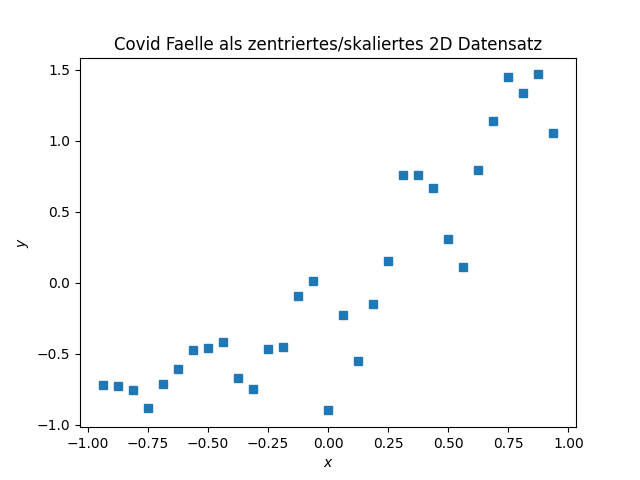
\includegraphics[width=0.65\textwidth,height=\textheight]{bilder/07-covid-cntrd.png}
\caption{Fallzahlen von Sars-CoV-2 in Bayern im Oktober
2020 -- zentriert}\label{fig:cases-cntrd}
}
\end{figure}

\hypertarget{variationskoeffizienten}{%
\subsection{Variationskoeffizienten}\label{variationskoeffizienten}}

Als nächstes kann Jan sich fragen, wie gut die Daten durch ihren Mittelwert beschrieben werden und die Varianzen berechnen, die für zentrierte Daten so aussehen

\begin{equation*}
s_x^2 = \frac {1}{N-1} \sum_{i=1}^N x_i^2,
\quad
s_y^2 = \frac {1}{N-1} \sum_{i=1}^N y_i^2.
\end{equation*}

Im gegebenen Fall bekommen wir
\begin{equation*}
s_x^2 \approx 0.32
\quad
s_y^2 \approx  0.57
\end{equation*}
und schließen daraus, dass in \(y\) Richtung \emph{viel passiert} und in \(x\) Richtung \emph{nicht ganz so viel}. Das ist jeder Hinsicht nicht befriedigend, wir können weder

\begin{itemize}
\tightlist
\item
  Redundanzen ausmachen (eine Dimension der Daten vielleicht weniger wichtig?) noch
\item
  dominierende Richtungen feststellen (obwohl dem Bild nach so eine offenbar existiert)
\end{itemize}

und müssen konstatieren, dass die Repräsentation der Daten im \((x,y)\) Koordinatensystem nicht optimal ist.

Die Frage ist also, ob es ein Koordinatensystem gibt, dass die Daten besser darstellt.

\leavevmode\hypertarget{rem-coors}{}%
\begin{JHSAYS}
Ein Koordinatensystem ist nichts anderes als eine Basis. Und die Koordinaten eines Datenpunktes sind die Komponenten des entsprechenden Vektors in dieser Basis. Typischerweise sind Koordinatensysteme orthogonal (das heißt eine Orthogonalbasis) und häufig noch orientiert (die Basisvektoren haben eine bestimmte Reihenfolge und eine bestimmte Richtung).

\end{JHSAYS}

\hypertarget{koordinatenwechsel}{%
\subsection{Koordinatenwechsel}\label{koordinatenwechsel}}

Sei nun also \(\{b_1,b_2\}\subset \mathbb R^{2}\) eine orthogonale Basis.

\leavevmode\hypertarget{rem-ortho-bas}{}%
\begin{JHSAYS}
Wie allgemein gebräuchlich, sagen wir \emph{orthogonal}, meinen aber \emph{orthonormal}. In jedem Falle soll gelten
\begin{equation*}
b_1^T b_1=1, \quad b_2^Tb_2=1, \quad b_1^Tb_2 = b_2^Tb_1 = 0.
\end{equation*}

\end{JHSAYS}

Wir können also alle Datenpunkte
\(\mathbf x_i = \begin{bmatrix} x_i \\ y_i \end{bmatrix}\)
in der neuen Basis darstellen mit eindeutig bestimmten Koeffizienten \(\alpha_{i1}\) und \(\alpha_{i2}\) mittels
\begin{equation*}
\mathbf x_i = \alpha_{i1}b_1 + \alpha_{i2}b_2.
\end{equation*}
Für orthogonale Basen sind die Koeffizienten durch \emph{testen} mit dem Basisvektor einfach zu berechnen:
\begin{align*}
b_1^T\mathbf x_i = b_1^T(\alpha_{i1}b_1 + \alpha_{i2}b_2) = \alpha_{i1}b_1^Tb_1 + \alpha_{i2}b_1^Tb_2 = \alpha_{i1}\cdot 1 + \alpha_{i2} \cdot 0 = \alpha_{i1},\\
b_2^T\mathbf x_i = b_2^T(\alpha_{i1}b_1 + \alpha_{i2}b_2) = \alpha_{i1}b_1^Tb_2 + \alpha_{i2}b_2^Tb_2 = \alpha_{i1}\cdot 0 + \alpha_{i2}\cdot 1 = \alpha_{i2}.
\end{align*}
Es gilt also
\begin{equation*}
\alpha_{i1} = b_1^T\mathbf x = b_1^T\begin{bmatrix}
x_i \\ y_i
\end{bmatrix}, \quad
\alpha_{i2} = b_2^T\mathbf x_i = b_2^T\begin{bmatrix}
x_i \\ y_i
\end{bmatrix}.
\end{equation*}

Damit, können wir jeden Datenpunkt \(\mathbf x_i=(x_i, y_i)\) in den neuen Koordinaten \((\alpha_{i1}, \alpha_{i2})\) ausdrücken.

Zunächst halten wir fest, dass auch in den neuen Koordinaten die Daten zentriert sind. Es gilt nämlich, dass
\begin{align*}
\frac 1N \sum_{i=1}^N \alpha_{ji}=\frac 1N \sum_{i=1}^N b_j^T\mathbf x_i 
=\frac 1N b_j^T \sum_{i=1}^N \begin{bmatrix} x_i \\ y_i \end{bmatrix}
=& \frac 1N b_j^T \begin{bmatrix} \sum_{i=1}^N x_i \\ \sum_{i=1}^N y_i \end{bmatrix}\\
&=b_j^T \begin{bmatrix} \frac 1N \sum_{i=1}^N x_i \\ \frac 1N \sum_{i=1}^N y_i \end{bmatrix}
=b_j^T \begin{bmatrix} 0 \\ 0 \end{bmatrix} = 0,
\end{align*}
für \(j=1,2\).

Desweiteren gilt wegen der Orthogonalität von \(B=[b_1~b_2]\in \mathbb R^{2\times 2}\), dass
\begin{equation*}
x_{i}^2 + y_{i}^2 = \|\mathbf x_i\|^2 = \|B^T\mathbf x_i\|^2 
= \|\begin{bmatrix} b_1^T \\ b_2^T \end{bmatrix} \mathbf x_i\|^2
= \|\begin{bmatrix} b_1^T\mathbf x \\ b_2^T\mathbf x \end{bmatrix}\|^2
= \|\begin{bmatrix} \alpha_{i1} \\ \alpha_{i2} \end{bmatrix}\|^2
= \alpha_{i1}^2 + \alpha_{i2}^2
\end{equation*}
woraus wir folgern, dass in jedem orthogonalen Koordinatensystem, die Summe der beiden Varianzen die gleiche ist:
\begin{equation*}
s_x^2 + s_y^2 = \frac{1}{N-1}\sum_{i=1}^N(x_i^2 + y_i^2) = \frac{1}{N-1}\sum_{i=1}^N(\alpha_{i1}^2 + \alpha_{i2}^2) =: s_1^2 + s_2^2.
\end{equation*}

Das bedeutet, dass durch die Wahl des Koordinatensystems die Varianz als Summe nicht verändert wird. Allerdings können wir das System so wählen, dass eine der Varianzen in Achsenrichtung maximal wird (und die übrige(n) entsprechend klein).

Analog gilt für den eigentlichen Mittelwert der (nichtzentrierten) Daten, dass die Norm gleich bleibt. In der Tat, für die \emph{neuen} Koordinaten des Mittelwerts gilt in der Norm
\begin{equation*}
\|
\begin{bmatrix}
\alpha_{c1} \\ \alpha_{c2}
\end{bmatrix}
\|
=
\|
B^T
\begin{bmatrix}
x_c \\ y_c
\end{bmatrix}
\|
=
\|
\begin{bmatrix}
x_c \\ y_c
\end{bmatrix}
\|.
\end{equation*}

\hypertarget{sec-pca-maximierung}{%
\subsection{Maximierung der Varianz in (Haupt)-Achsenrichtung}\label{sec-pca-maximierung}}

Wir wollen nun also \(b_1\in \mathbb R^{2}\), mit \(\|b_1\|=1\) so wählen, dass
\begin{equation*}
s_1^2 = \frac{1}{N-1}\sum_{i=1}^n \alpha_{i1}^2
\end{equation*}
maximal wird. Mit der Matrix \(\mathbf X\) aller Daten
\begin{equation*}
\mathbf X = \begin{bmatrix}
x_1 & y_1 \\ x_2 & y_2 \\ \vdots & \vdots \\ x_N & y_N
\end{bmatrix} = 
\begin{bmatrix}
\mathbf x_1^T\\ \mathbf x_2^T  \\  \vdots \\ \mathbf x_N^T
\end{bmatrix} 
\in \mathbb R^{N\times 2}
\end{equation*}
können wir die Varianz in \(b_1\)-Richtung kompakt schreiben als
\begin{equation*}
s_1^2 = \frac{1}{N-1}\sum_{i=1}^n \alpha_{i1}^2
= \frac{1}{N-1}\sum_{i=1}^n (b_1^T\mathbf x_i)^2
= \frac{1}{N-1}\sum_{i=1}^n (\mathbf x_i^Tb_1)^2
= \frac{1}{N-1}\| \mathbf X b_1 \|^2
\end{equation*}
Wir sind also ein weiteres mal bei einem Optimierungsproblem (diesmal mit Nebenbedingung) angelangt:
\begin{equation}\label{eq:eqn-max-varianz}
\max_{b\in \mathbb R^{2},\, \|b\|=1} \|\mathbf X b\|^2
\end{equation}

\begin{lemma}[Maximale Varianz]
\protect\hypertarget{lem:varianz-maximization}{}\label{lem:varianz-maximization}Die Lösung des Varianz-Maximierungsproblem \eqref{eq:eqn-max-varianz} ist mit \(b=v_1\) gegeben, wobei \(v_1\) der erste (rechte) Singulärvektor von \(\mathbf X\) ist:
\begin{equation*}
\mathbf X = U \Sigma V^T = U \Sigma \begin{bmatrix}
v_1^T \\ v_2^T
\end{bmatrix}.
\end{equation*}
\end{lemma}

\begin{proof}
Ein etwas indirekter Beweis basiert auf der Feststellung dass in
\eqref{eq:eqn-max-varianz} genau die 2-Norm der Matrix \(X\) gesucht ist und dass
bei \(v_1\) das Maximum realisiert wird.
\end{proof}

Damit rechnen wir auch direkt nach, dass im neuen Koordinatensystem \(\{b_1, b_2\}=\{v_1, v_2\}\) die Varianzen \(s_1^2\) und \(s_2^2\) (bis auf einen Faktor von \(\frac{1}{N-1}\)) genau die quadrierten Singulärwerte von \(\mathbf X\) sind:
\begin{align*}
(N-1)s_1^2 
= \|\mathbf X v_1 \|^2 = \|U \Sigma \begin{bmatrix} v_1^T \\ v_2^T \end{bmatrix}v_1\|^2
= \|\Sigma \begin{bmatrix} v_1^Tv_1 \\ v_2^T v_1\end{bmatrix}\|^2
=  \|\Sigma \begin{bmatrix} 1 \\  0\end{bmatrix}\|^2
=\sigma_1^2,\\
(N-1)s_2^2 
= \|\mathbf X v_2 \|^2 = \|U \Sigma \begin{bmatrix} v_1^T \\ v_2^T \end{bmatrix}v_2\|^2
= \|\Sigma \begin{bmatrix} v_1^Tv_2 \\ v_2^T v_2\end{bmatrix}\|^2
=  \|\Sigma \begin{bmatrix} 0 \\  1\end{bmatrix}\|^2
=\sigma_2^2
\end{align*}

Für unser Covid Beispiel ergibt sich
\begin{equation*}
V^T \approx
\begin{bmatrix}
0.5848 &  0.8111 \\
0.8111 & -0.5848
\end{bmatrix}
\end{equation*}
also
\begin{equation*}
b_1 = v_1 = \begin{bmatrix}
0.5848 \\  0.8111 
\end{bmatrix}
\quad
b_2 = v_2 = \begin{bmatrix}
0.8111 \\ -0.5848
\end{bmatrix}
\end{equation*}
als neue Koordinatenrichtungen mit
\begin{equation*}
s_1^2 \approx 0.85, \quad s_2^2 \approx 0.04,
\end{equation*}
was bereits eine deutliche Dominanz der \(v_1\)-Richtung -- genannt \emph{Hauptachse} -- zeigt.

Im Hinblick auf Anwendungen und Eigenschaften der PCA untersuchen werden, noch ein Plot der Daten mit der \(v_1\)-Richtung als Linie eingezeichnet.

\begin{figure}
\hypertarget{fig:cases-cntrd-HA}{%
\centering
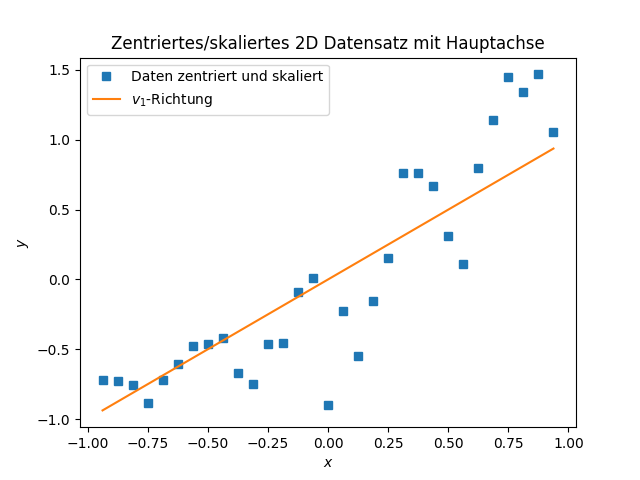
\includegraphics[width=0.65\textwidth,height=\textheight]{bilder/07-covid-cntrd-HA.png}
\caption{Fallzahlen von Sars-CoV-2 in Bayern im Oktober
2020 -- zentriert/skaliert/Hauptachse}\label{fig:cases-cntrd-HA}
}
\end{figure}

\hypertarget{support-vector-machines}{%
\chapter{Support Vector Machines}\label{support-vector-machines}}

\newcommand\ipro[2]{\bigl \langle #1, \, #2\bigr\rangle }

In diesem Kapitel betrachten wir, wie das Klassifizierungsproblem (erstmal
bezüglich zweier Merkmale) durch eine optimale Wahl einer trennenden
Hyperebene gelöst werden kann.
In der Tat sind die Merkmale der SVM

\begin{itemize}
\tightlist
\item
  dass die \emph{beste} Hyperebene
\item
  effizient berechnet wird
\item
  und das sogar für möglicherweise nichtlineare Einbettungen in
  höhere Dimensionen (\emph{kernel-SVM})
\end{itemize}

\begin{figure}
\hypertarget{fig:cases-cntrd-HA}{%
\centering
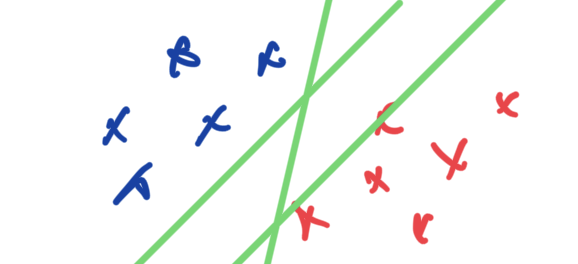
\includegraphics[width=0.65\textwidth,height=\textheight]{bilder/08_hyperebene-punkte-bsp.png}
\caption{Beispiel Illustration von Punktwolken mit zwei verschiedenen Labels (hier rot
und blau) und verschiedener trennender Hyperebenen}\label{fig:cases-cntrd-HA}
}
\end{figure}

\hypertarget{problemstellung}{%
\section{Problemstellung}\label{problemstellung}}

\begin{definition}[Problemstellung für die SVM]
\protect\hypertarget{def:def-svm-problem}{}\label{def:def-svm-problem}\leavevmode

\begin{enumerate}
\def\labelenumi{\arabic{enumi}.}
\item
  Gegeben sei eine Wolke im \(\mathbb R^{n}\) von \(N\) Datenpunkten \[\mathbb X :=
  \bigl \{(x_i,y_i)\colon x_i \in \mathbb R^{n}, \, y_i\in \{-1,+1\}, \,
  i=1,\dotsc, N\bigr \}\] wobei \(x_i\) der Datenpunkt ist und \(y_i\) das
  zugehörige Label.
\item
  Eine \emph{Hyperebene} \(H\subset \mathbb R^{n}\), definiert durch den
  Stützvektor \(b\subset \mathbb R^{n}\) und den Normalenvektor \(w\in \mathbb R^{n}\), heißt \textbf{trennend}, falls
  \begin{equation}\label{eq:eqn-trennende-hyperebene}
  y_i\bigl \langle x_i-b, \, w\bigr\rangle  >0, \quad i=1,\dotsc,N
  \end{equation}
\item
  Die Hyperebene \(H\) heißt \emph{Support Vector Machine} falls, \(H\) die
  Hyperebene ist, für die der \textbf{kleinste} Abstand
  \[d(H, \mathbb X) = \min_{s\in H, i=1, \dotsc, N}\{\|s-x_i\|_2\}\]
  \textbf{maximal} wird.
\end{enumerate}

\end{definition}

Ein Paar Bemerkungen dazu.

\begin{enumerate}
\def\labelenumi{\arabic{enumi}.}
\tightlist
\item
  Dass die Labels mit \(\pm 1\) gewählt werden hat ganz praktische
  Gründe:
\item
  Zunächst lässt sich anhand des Vorzeichen des inneren Produktes
  \(\bigl \langle x-b, \, w\bigr\rangle \) entscheiden, auf \emph{welcher Seite} von \(H\) ein Punkt \(x\) liegt.
  (Punkte auf der gleichen Seite haben das gleiche Vorzeichen). Mit der Wahl
  der labels als \(\pm 1\) kann das kompakt in einer einzigen Gleichung wie
  in \eqref{eq:eqn-trennende-hyperebene}
  in der Definition geschrieben werden.
\item
  Ist die Hyperebene bekannt, können neue Datenpunkte \(x\) über das
  Vorzeichen von \(\bigl \langle x-b, \, w\bigr\rangle \) gelabelt werden -- das ist die eigentliche
  Motivation, diese Hyperebene möglichst gut zu bestimmen.
\item
  Es gilt \(\bigl \langle x-b, \, w\bigr\rangle =\bigl \langle x, \, w\bigr\rangle -\bigl \langle b, \, w\bigr\rangle :=\bigl \langle x, \, w\bigr\rangle  -\beta\). Und damit
  genügt es zur Definition (und zum Einsatz in der Klassifizierung), nur
  den Vektor \(w\in \mathbb R^{n}\) und den \emph{bias} \(\beta \in \mathbb R^{}\) zu
  bestimmen (beziehungsweise zu kennen).
\item
  Klassischere Methoden zur Klassifizierung mittels Hyperebene benutzen
  beispielsweise einfache neuronale Netze um ein passendes \((w, \beta)\) zu bestimmen.
\item
  Eine solche Hyperebene kann durchaus auch \textbf{nicht existieren}, dann
  heißen die Daten \emph{nicht linear trennbar}. Existiert eine solche Ebene,
  dann existieren unendlich viele -- ein weiterer Grund, die Ebene optimal (und
  damit hoffentlich eindeutig) zu wählen.
\end{enumerate}

\hypertarget{maximierung-des-minimalen-abstands}{%
\section{Maximierung des Minimalen Abstands}\label{maximierung-des-minimalen-abstands}}

Um den Abstand maximieren zu können leiten wir eine Formel her.

Dazu sei \(w\in \mathbb R^{n}\) der Normalenvektor von \(H\) sei \(h\in \mathbb R^{}\)
so, dass \(b=\frac{h}{\|w\|}w\) ein Stützvektor ist. (Insbesondere kann Jan eine
Hyperebene auch über den Normalenvektor und den Abstand von \(H\) zum
Ursprung charakterisieren). Damit bekommen wir den Abstand von \(H\) zum Ursprung
als \(h\) (Achtung: das \(h\) kann auch negativ sein -- es sagt uns wie weit
müssen wir den normalisierten Vektor \(w\) entlanglaufen, bis wir zu Ebene
\(H\) gelangen).

Zu einem beliebigen Punkt \(x\in \mathbb R^{n}\) bekommen wir den Abstand zu \(H\)
als

\begin{itemize}
\tightlist
\item
  den Abstand der Ebene \(H\) zur Ebene \(H_x\), die parallel zu \(H\) verläuft
  und \(x\) enthält
\item
  beziehungsweise als die Differenz der Abstände von \(H_x\) und \(H\) zum Ursprung
\end{itemize}

Da auch \(w\) der Normalenvektor von \(H_x\) ist, gilt für den Abstand \(h'\),
dass
\begin{equation*}
h_x = \|x\|_2\cos(\phi(w,x))=\|x\|_2 \frac{\bigl \langle w, \, x\bigr\rangle  }{\|w\|_2\|x\|_2} = \frac{\bigl \langle w, \, x\bigr\rangle }{\|w\|_2}
\end{equation*}
wobei
\(\cos(\phi(w, x))\)
aus dem Winkel zwischen \(x\) und \(w\) herrührt.

Mit dieser Formel und mit \(b=hw\), erkennen wir, dass der Test auf das Vorzeichen
\begin{equation*}
\bigl \langle x-b, \, w\bigr\rangle  = \bigl \langle x-\frac{h}{\|w\|_2} w, \, w\bigr\rangle  = \bigl \langle x, \, w\bigr\rangle  - h\|w\|_2
= \|w\|_2 (\frac{\bigl \langle x, \, w\bigr\rangle  }{\|w\|_2} - h) = \|w\|_2(h_x - h)
\end{equation*}
den mit \(\|w\|_2\) skalierten Abstand (inklusive dem Vorzeichen) enthält,
beziehungsweise, dass der Abstand als
\begin{equation*}
y_i\frac{\bigl \langle x_i-b, \, w\bigr\rangle }{\|w\|_2} = y_i\frac{\bigl \langle x_i, \, w\bigr\rangle -\beta}{\|w\|_2}
\end{equation*}
(für eine trennende Hyperebene \((w, \beta)\)) auch immer das richtige Vorzeichen erhält (da \(\|w\|_2>0\). Dementsprechend kann das SVM Problem als
\begin{equation*}
\max_{w\in \mathbb R^{n}, \, \beta \in \mathbb R^{}} \min_{x_i \in \mathbb X} y_i\frac{\bigl \langle x_i, \, w\bigr\rangle -\beta}{\|w\|_2}
\end{equation*}
formuliert werden.

So ein \(\min \max\) Problem ist generell schwierig zu analysieren und zu
berechnen. Aber wir können direkt sagen, dass die \emph{Zulässigkeit} der Optimierung gesichert
ist, da ``der \(\max\)-imierer'' nach Möglichkeit eine trennende Hyperebene
wählt und so schon mal sicherstellt, dass ``der \(\min\)-inimierer'' nur
über positive Zahlen minimiert.

Darüberhinaus, wenn eine trennendes Hyperebene existiert, sodass
\begin{equation*}
y_i(\bigl \langle x_i, \, w\bigr\rangle -\beta) = y_i(\bigl \langle x_i, \, w\bigr\rangle  -h \|w\|_2) \geq q > 0
\end{equation*}
dann können wir durch die Wahl von \(\tilde w =\frac 1q w\), immer
erreichen, dass das Minimum \(\min_{ x_i \in \mathbb X} y_i \bigl \langle x_i, \, w\bigr\rangle -\beta=1\) ist und das Max-Min durch ein Maximierungsproblem unter Zulässigkeitsnebenbedingungen
\begin{equation*}
\min_{w,\beta} \frac 12 \|w\|_2^2, \quad{s.t.}\quad y_i(\bigl \langle x_i, \, w\bigr\rangle -\beta) \geq 0, \,
i=1,\dotsc, N
\end{equation*}
ersetzen. Dabei haben wir noch ausgenutzt, dass \(\max_w \frac 1{\|w\|}\leftrightarrow \min_w \frac 12 \|w\|^2\) entspricht, um die Standardform
eines \emph{quadratischen Optimierungsproblems} unter (affin) \emph{linearen
Ungleichungsnebenbedingungen} zu erhalten.

Für solche Optimierungsprobleme kann das \emph{duale Problem} direkt hergeleitet
werden, was sich in diesem Fall als die Suche eines Vektors \(a\in \mathbb R^{n}\)
über das restringierte Minimierungsproblem
\begin{equation*}
\min_{a} \left(\frac 12 \sum_{i=1}^N\sum_{k=1}^Na_ia_k y_i y_k \bigl \langle x_i, \, x_k\bigr\rangle  -
\sum_{i=1}^N a_i\right) \quad{s.t.}\quad a\geq0, \, \sum_{i=1}^Na_iy_i=0
\end{equation*}
ergibt.

Aus der KKT Theorie kann abgeleitet werden, dass \(a_i>0\), genau dann wenn \(x_i\)
die Gleichheit \(y_i(\bigl \langle x_i, \, w\bigr\rangle -\beta)=1\) erfüllt ist, also \(x_i\) ein
sogenannter \emph{support vector} ist. Ist \(S\) die Menge aller Indices, die die
\emph{support vectors} indizieren, so kann die Klassifikation eines neuen
Datenpunktes \(x\) mittels
\begin{equation*}
y(x) = \sum_{i\in S}a_iy_i\bigl \langle x, \, x_i\bigr\rangle +\gamma
\end{equation*}
vorgenommen werden, wobei der \emph{bias} als
\begin{equation*}
\gamma = \sum_{i\in S}(y_i - \sum_{k\in S}a_ky_k\bigl \langle x_i, \, x_k\bigr\rangle )
\end{equation*}
vorberechnet werden kann.

\hypertarget{nichtlineare-separation}{%
\subsection{Nichtlineare Separation}\label{nichtlineare-separation}}

Existiert auf den Originaldaten keine separierende Hyperebene (oder ist sie schwer zu berechnen) dann
können die Daten in höhere Dimensionen nichtlinear eingebettet werden
und dort separiert werden.

\begin{equation*}
\Psi \colon \mathbb R^{n} \to \mathbb R^{M}
\end{equation*}

Beispiel von gestern
\begin{equation*}
\Psi\colon \mathbb R^{} \to \mathbb R^{2}\colon x \to \Psi(x) = (x, (x-2)^2)
\end{equation*}

Mit der erhöhten Dimension kommen zwei Aufgaben mit einer Lösung

\begin{enumerate}
\def\labelenumi{\arabic{enumi}.}
\item
  Die transformierten Daten müssen separiert und neue Daten müssen
  klassifiziert werden -- das ist schwierig und aufwändig für \(N\gg 1\).
\item
  Wie soll \(\Psi\) gewählt werden?
\end{enumerate}

Die Lösung zu beidem ist, dass

\begin{enumerate}
\def\labelenumi{\arabic{enumi}.}
\tightlist
\item
  in der dualen Formulierung nur Skalarprodukte \(\bigl \langle x_i, \, x_j\bigr\rangle \)
  beziehungsweise \(\bigl \langle \Psi(x_i), \, \Psi(x_j)\bigr\rangle \) benötigt werden
\item
  die bestenfalls durch \emph{kernel} Funktionen einfach berechnet werden
  können (ohne das Lifting in den hochdimensionalen Raum)
\end{enumerate}

Beispiele:

\begin{itemize}
\tightlist
\item
  \(\Psi(x_1, x_2) = (x_1^2, \sqrt{2}x_1x_2, x_2^2)\) hat die \emph{kernel} Funktion
  \(k(x,y)=(x_1y_1+x_2y_2)^2\)
\end{itemize}

Damit wird zunächst das Berechnungsproblem gelöst. Das Problem, welche
Funktionen gewählt werden, wird nebenbei dadurch gelindert,
dass

\begin{enumerate}
\def\labelenumi{\arabic{enumi}.}
\tightlist
\item
  die Effizienz in der Auswertung \emph{try and error} möglich macht
\item
  Jan letztlich gar keine \(\Psi\)s mehr sucht, sondern nur noch \(k\)s mit
  bekannten Eigenschaften.
\end{enumerate}

\hypertarget{aufgaben-1}{%
\section{Aufgaben}\label{aufgaben-1}}

\begin{enumerate}
\def\labelenumi{\arabic{enumi}.}
\tightlist
\item
  Sei die Hyperebene über \(w\) und \(b\) gegeben. Bestimmen Sie den
  (möglicherweise negativen) Abstand
  \(h\in \mathbb R^{}\), sodass \(hw\in H\).
\end{enumerate}

\hypertarget{best-and-universal-approximation}{%
\chapter{Best and Universal Approximation}\label{best-and-universal-approximation}}

\def\PLab{\operatorname{PL}[a, b]}
\def\PCab{\operatorname{Pc}[a, b]}
\def\Cab{\mathcal{C}[a, b]}

Alle bisher betrachteten Approximationsprobleme waren in Bezug auf eine \emph{2-norm}
(``least squares'') formuliert. Die für die Berechnung unmittelbaren Vorteile
sind die

\begin{enumerate}
\def\labelenumi{\arabic{enumi}.}
\tightlist
\item
  Differenzierbarkeit der Norm und die
\item
  Charakterisierung der Optimallösung über Orthogonalität.
\end{enumerate}

Ein gängiges Optimierungsproblem, eine Bestapproximation zu einer stetigen
Funktion \(f\colon [a, b]\to \mathbb R^{}\) in einer passenden Menge von Funktionen
\(\mathcal G\) bezüglich der \emph{Supremumsnorm}\footnote{für ein kompaktes
  Intervall wird das zur \emph{Maximumsnorm}} zu finden
\begin{equation*}
\min_{g\in \mathcal G} \|f-g\|_\infty = 
\min_{g \in \mathcal G}\bigl (\max_{x\in [a, b]}|f(x)-g(x)|\bigr )
\end{equation*}
fällt nicht darunter.
Die entstehenden Schwierigkeiten und theoretische und praktische Ansätze
zur möglichen Lösung dieses sogenannten
\emph{Tschebyscheff-Approximation}-Problem, sind in (Kapitel 8.7.2, Richter and Wick \protect\hyperlink{ref-RicW17}{2017}) gut
nachzulesen.

\hypertarget{universal-approximation}{%
\section{Universal Approximation}\label{universal-approximation}}

Wir wollen hier nachvollziehen, dass klassische neuronale Netze, dieses Problem
approximativ aber mit beliebiger Genauigkeit \(\epsilon\) lösen könnten. Die
Schritte da hin sind wie folgt

\begin{enumerate}
\def\labelenumi{\arabic{enumi}.}
\item
  Zu einem gegebenen \(f\in \mathcal C[a, b]\) (einer reellwertigen, stetigen Funktion
  auf einem
  endlichen und abgeschlossenen Intervall) existiert immer eine stückweise
  konstante Funktion \(f_N\) mit endlich vielen \emph{Sprungstellen}, sodass
  \begin{equation*}
  \|f-f_N\|_\infty < \frac \epsilon2
  \end{equation*}
\item
  Zu diesem \(f_N\) können wir immer eine Funktion
  \begin{equation*}
  s_M(x) = c_0 + \sum_{i=1}^Mc_i \tanh (a_i(x - b_i))
  \end{equation*}
  konstruieren (durch Anpassung der Parameter \(c_0\), \(c_i\), \(b_i\), \(a_i\),
  \(i=1,\dotsc, M\)) sodass
  \begin{equation*}
  \|f_N-s_M\| < \frac \epsilon2.
  \end{equation*}
\item
  Wir interpretieren \(s_M\) als ein neuronales Netz mit einer \emph{hidden layer} und
  können konstatieren dass
  \begin{equation*}
  \|f-s_M\|_\infty \leq \|f-f_N\|_\infty + \|f_N-s_M\|_\infty < \frac \epsilon2
  + \frac \epsilon2 = \epsilon.
  \end{equation*}
\end{enumerate}

Einige Fragen werden wir unbeantwortet lassen müssen, vor allem

\begin{itemize}
\tightlist
\item
  wie wählen wir \(M\) (das Resultat sagt nur \(M\) muss groß genug
  sein)
\end{itemize}

und

\begin{itemize}
\tightlist
\item
  wie wirkt sich in der Praxis die approximative Berechnung von \(a_i\)--\(c_i\)
  auf die Approximation aus?
\end{itemize}

Dennoch gibt dieses Beispiel einen Einblick in die Funktionsweise der
Approximation und das referenzierte \emph{universal
approximation theorem} ist Grundlage vieler Analyseansätze für
neuronale Netzwerke.

In Schritt 1, wird die stückweise konstante Funktion \(f_N\) definiert. Die
Existenz folgt aus dem Satz

\begin{theorem}[Approximation durch stückweise konstante Funktionen]
\protect\hypertarget{thm:thm-pc-dense-C}{}\label{thm:thm-pc-dense-C}Sei \([a, b]\subset \mathbb R^{}\) ein abgeschlossenes endliches Intervall.
Der Abschluss bezüglich der Supremumsnorm der Menge \(\operatorname{Pc}[a, b]\) aller stückweise konstanten Funktionen auf \([a, b]\) mit endlich vielen Sprungstellen \textbf{enthält} \(\mathcal C[a, b]\), d.h.
\begin{equation*}
\mathcal{C}[a, b]\subset \operatorname{closure}_{\|\cdot\|_\infty}(\operatorname{Pc}[a, b]).
\end{equation*}
Insbesondere, existiert für ein beliebiges \(f\in \mathcal C[a, b]\) und \(\varepsilon > 0\), immer ein \(g\in \operatorname{Pc}[a, b]\) mit \(\|f-g\|_\infty<\varepsilon\).
\end{theorem}

\begin{proof}
Der Beweis ist klassisch -- hier nur die relevanten und konstruktiven Elemente.

An sich muss gezeigt werden, dass es zu jeder Funktion \(f\in \mathcal C[a, b]\) eine Folge \(\{f_n\}\subset \operatorname{Pc}[a, b]\) gibt, mit \(f\) als Grenzwert. Wir
zeigen nur die Konstruktion eines potentiellen Folgengliedes.

Sei \(f\in \mathcal{C}[a, b]\) beliebig. Da stetige Funktionen auf kompakten Mengen
gleichmäßig stetig sind, gibt es zu jedem \(\varepsilon>0\) ein \(\delta>0\), sodass
\begin{equation*}
|f(x\pm h) - f(x)| < \varepsilon
\end{equation*}
für alle \(h<\delta\). Damit können wir zu jedem \(\varepsilon\) eine
Unterteilung von \((a, b]\) in \(N(\delta)\) halboffene (bis auf das abgeschlossene
``erste'' Intervall, das \(a\) enthält) disjunkte Intervalle \(I_j\),
\(j=1, \dotsc, N(\delta)\) finden, sodass
\begin{equation*}
f_N(x) = \sum_{j=1}^N\chi_{I_j}(x)
\end{equation*}
\end{proof}

mit den Indikatorfunktionen \(\chi_{I_j}\) und mit
\begin{equation*}
f_j = \frac 12 (\max_{\xi\in I_j}\{f(\xi)\}+\min_{\eta \in I_j}\{f(\eta)\})
\end{equation*}
eine Funktion aus \(\operatorname{PL}[a, b]\) darstellt, die um maximal \(\varepsilon\) von \(f\)
abweicht. Außerdem können wir damit sicherstellen, dass
\begin{equation}\label{eq:eqn-fj-fjp-se}
|f_{j} - f_{j+1}| < \varepsilon,
\end{equation}
für alle \(j=1, \dotsc, N-1\) gilt, was im nächsten Schritt
relevant wird.

In Schritt 2 wird nun die Funktion \(f_N\) durch Linearkombinationen von
transformierten \(\tanh\) Funktionen approximiert:
\begin{equation*}
f_N(x) \approx g_M(x) := c_0 + \sum_{i=1}^Mc_i\tanh(a_i(x-b_i))
\end{equation*}

\begin{figure}
\hypertarget{fig:sum-tanhs}{%
\centering
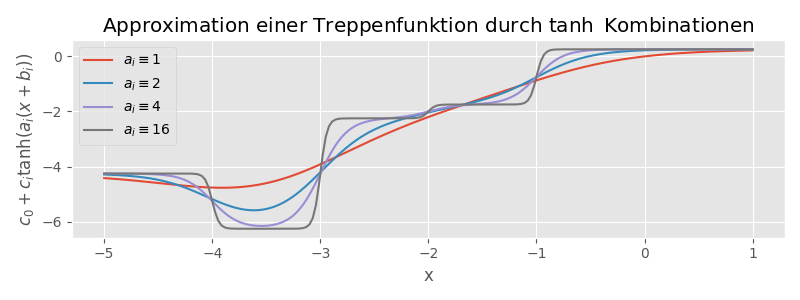
\includegraphics[width=0.95\textwidth,height=\textheight]{bilder/09-sumtanhs.png}
\caption{Beispiel Illustration wie eine Linearkombination von skalierten \(\tanh\) Funktionen eine Treppenfunktion approximiert}\label{fig:sum-tanhs}
}
\end{figure}

Die Konstruktion und der Nachweis, dass für jedes \(\varepsilon<0\) (mit \(f_N\) bereits entsprechend konstruiert) eine Differenz \(\|f_N - g_M\|_\infty < \varepsilon\) möglich ist, basiert auf folgenden Argumenten:

\begin{itemize}
\item
  Allgemein gilt für die Funktion \(\tanh\), dass sie \emph{streng monoton} ist,
  dass \(\tanh(0)=0\) und dass \(\lim_{x\to \pm \infty} \tanh(x) = \pm 1\).
\item
  Durch eine Skalierung von \(x\leftarrow ax\) mit \(a\to \infty\), passiert der übergang von \(-1\) zu \(1\)
  beliebig schnell -- \(\tanh\) entspricht zunehmend der Treppenfunktion, die
  bei \(0\) von \(-1\) auf \(+1\) springt. (Jan bemerke, dass diese ``Konvergenz''
  \textbf{nicht} bezüglich der \emph{Supremumsnorm} stattfindet.)
\item
  Durch einen Shift \(x \leftarrow x-b\) kann der Sprung von \(x=0\) zu \(x=b\)
  verschoben werden.
\item
  Durch Skalierung \(\tanh \leftarrow c\tanh\) kann die Höhe des Sprungs
  angepasst werden.
\end{itemize}

Damit (und insbesondere mit \(b_i\) als die Sprungstellen von \(f_N\) gewählt
und \(c_i\) als die Differenz zwischen den Werten an diesem Sprung), kann direkt
ein \(g_M\) konstruiert werden, das bis auf beliebig kleine, offene Umgebungen um die
Sprungstellen dem \(f_N\) beliebig nahe kommt. (Allerdings nicht in der
\emph{Supremumsnorm}).
Da für genügend große \(a_i\) aber sichergestellt wird, dass \(g_M\)
auf jedem Teilintervall zwischen den Werten von \(f_N\) interpoliert, folgt aus
\eqref{eq:eqn-fj-fjp-se},
dass auch die punktweise Differenz kleiner als \(\varepsilon\)
ist.
Insgesamt folgt so die Existenz von \(g_M\) mit den gewünschten
Eigenschaften.

Im letzten Schritt 3 interpretieren wir die \(g_M\) Approximation als ein neuronales
Netz.

Dazu bemerken wir, dass wir \(g_M\) schreiben können als
\begin{equation}\label{eq:eqn-gm-approx}
g_M(x) = c_0 + c^T \tanh(Ax+b)
\end{equation}
mit
\begin{equation*}
c=
\begin{bmatrix}
c_1 \\ c_2 \\ \vdots \\ c_M
\end{bmatrix}, 
\quad
A=
\begin{bmatrix}
a_1 \\ a_2 \\ \vdots \\ a_M
\end{bmatrix}, 
\quad
b=
\begin{bmatrix}
-a_1b_1 \\ -a_2b_2 \\ \vdots \\ -a_Mb_M
\end{bmatrix}
\end{equation*}
und der \emph{eintragsbezogenen} Interpretation der eigentlich skalaren \(\tanh\)
Funktion und dass

\begin{itemize}
\tightlist
\item
  der Anteil
  \begin{equation*}
  \tanh (Ax+b)
  \end{equation*}
  eine klassische \emph{linear layer} mit Aktivierung ist
\item
  während der Ausgang \(y=c_0+c^T\xi\) eine einfache lineare Abbildung (ohne
  Aktivierung ist).
\end{itemize}

In dieser Darstellung, ist die Suche nach den Parametern für \(g_M\) in den
Standardroutinen von \emph{ML} Paketen ohne weiteres möglich.

Wir schließen mit einigen allgemeinen Bemerkungen

\begin{itemize}
\tightlist
\item
  die Funktion \(\tanh\) hat durchaus Relevanz in der Praxis. Für die
  Theorie, die im wesentlichen Beschränktheit und Monotonie voraussetzt,
  gehen auch die gerne verwendeten allgemeineren \emph{sigmoid} Funktionen.
\item
  die größte Lücke zur Praxis ist die Annahme \emph{\(M\) genügend
  groß}. Etwas unpraktisch ist auch, dass nur eine \emph{hidden layer}
  verwendet wird. Neuere Arbeiten behandeln ähnliche
  Approximationsresultate mit mehreren Schichten.
\item
  die theoretisch unschönste Lücke ist die Annahme, dass eine Funktion
  auf einer kompakten Menge approximiert wird (was beispielsweise in der
  Behandlung von dynamischen Systemen nachteilig ist)
\item
  Zur Approximation von \(f_N\) ist Jan geneigt, die \(a_i\) einfach sehr groß
  zu wählen. Ist \(f\) stetig, dann werden allerdings bessere Resultate (die
  den Verlauf von \(f\) nachzeichnen) mit kleineren \(a_i\) erreicht. Außerdem
  führen große Werte von \(a\) zum sogenannten \emph{vanishing gradients}
  Phänomen, da \(\frac{\tanh(a(x+h))-\tanh(ax)}{h}\to 0\) für \(a\to \infty\).
\end{itemize}

\hypertarget{aufgaben-2}{%
\section{Aufgaben}\label{aufgaben-2}}

Zur Approximation einer Funktion \(f\colon \mathbb  R^{}\to \mathbb R^{}\) über den Ansatz \eqref{eq:eqn-gm-approx} seien
Datenpunkte \(\mathbb X = \{(x_i, y_i)\}_i\) mit \(y_i=f(x_i)\) gegeben und das
Optimierungsproblem
\begin{equation*}
   L(c, A, b; \mathbb X) = \sum_{i} \|y_i - g_M(c, A, b;\, x_i)\|_2^2 \to \min_{c, A, b}
   \end{equation*}
mittels des stochastischen Gradientenabstiegs zu lösen.

\begin{enumerate}
\def\labelenumi{\arabic{enumi}.}
\item
  Schreiben Sie die Koeffizienten in einen Vektor \(p=(c, A, b)\) und berechnen
  Sie \(\nabla_{c_0}L(p; \mathbf x)\), sowie beispielhaft die Komponenten
  von \(\nabla_p L(p; \mathbf x)\) für einen einzelnen Datenpunkt \(\mathbf x = x_i\) oder einen \emph{batch} \(\mathbf x = \mathbb x\) (wie es für den stochastischen
  Gradienten benutzt würde).
\item
  Formulieren Sie die Berechnung des Gradienten (bezüglich \(p\)) für
  \(M=1\) und einen Datenpunkt \(x\), also für die Funktion \(l = L(c_0, c_1, a_1, b_1; x)\) über \emph{automatisches Differenzieren} im Vorwärts-- und
  im Rückwärtsmodus.
\item
  Implementieren Sie die Approximation und das Training. Dafür können
  die Bausteine aus \protect\hyperlink{beispiel-implementierung}{Beispiel Implementierung} verwendet werden. Implementieren
  Sie auch die Gradientenberechnung zur Verwendung im stochastischen
  Abstiegsverfahren. Testen Sie ihre Implementierung für verschiedene \(M\)
  und verschiedene Daten für die Funktionen
  \begin{equation*}
  f_1(x)=\chi_{[-1, 0]}(x) - \chi_{(0, \frac 13]}(x)+ \chi_{(\frac 13, \frac 12]}(x) -
  \chi_{(\frac 12, 1]}(x), \quad f_2(x) = \sin(4x)
  \end{equation*}
  jeweils auf dem Intervall \([-1, 1]\).
\end{enumerate}

\hypertarget{automatisches-algorithmisches-differenzieren}{%
\chapter{Automatisches (Algorithmisches) Differenzieren}\label{automatisches-algorithmisches-differenzieren}}

In der Mathematik und im Bereich der Computeralgebra ist das \emph{automatische
Differenzieren} (auch \emph{Auto-Differenzieren}, \emph{Autodiff} oder einfach \emph{AD}
genannt und in anderen communities als \emph{algorithmisches Differenzieren} oder
\emph{computergestütztes Differenzieren} bezeichnet), ein Satz von Techniken zur
Berechnung (der Werte(!)) der partiellen Ableitung einer durch ein
Computerprogramm spezifizierten Funktion.

AD nutzt die Tatsache, dass jede Computerberechnung,
egal wie kompliziert, eine Sequenz von elementaren arithmetischen Operationen
(Addition, Subtraktion, Multiplikation, Division usw.) und elementaren
Funktionen (exp, log, sin, cos usw.) ausführt. Durch wiederholte Anwendung der
Kettenregel auf diese Operationen können partielle Ableitungen beliebiger
Ordnung automatisch, genau bis zur Arbeitspräzision und mit höchstens einem
kleinen konstanten Faktor mehr an arithmetischen Operationen als das
ursprüngliche Programm berechnet werden.

\hypertarget{andere-differentiationsmethoden}{%
\section{Andere Differentiationsmethoden}\label{andere-differentiationsmethoden}}

In manchen Anwendungsfällen wird auf eine symbolische Repräsentation von
Funktionen und Variablen in der computergestützten Berechnung
zurückgegriffen. Sogenannte Computeralgebra Pakete wie \texttt{Maple},
\texttt{Mathematica} oder die \emph{Python} Bibliotheken \texttt{SageMath} oder \texttt{Sympy} können
dann automatisiert auch Operationen auf Funktionen wie Integralberechnung und
eben auch Differentiation \emph{exakt} ausführen. Durch die Kettenregel und
unter der Massgabe, dass alle Codes letztlich nur elementare Funktionen mit
bekannten Ableitungen verschalten, wäre es auch möglich, bei
entsprechender Implementierung des primären Progamms, auch automatisiert
die Ableitungen zu erzeugen. Allerdings ist der Mehraufwand in der symbolischen
Programmierung erheblich und die Auswertung der Ausdrücke langsam, sodass
symbolische Berechnungen (und entsprechend auch die Möglichkeit der
symbolischen automatischen Differentiation) nur in spezifischen und insbesondere
nicht in ``grossen'' und ``multi-purpose'' Algorithmen zur Anwendung kommen.

\leavevmode\hypertarget{ad-vs-sd}{}%
\begin{JHSAYS}
Auch AD rechnet symbolisch und rekursiv mit der Kettenregel. Der Unterschied ist, dass AD nur mit Funktionswerten der
Ableitungen arbeitet während die symbolische Ableitung versucht, die
Ableitung als Funktion zu erzeugen.

\end{JHSAYS}

Auf der anderen Seite steht die \emph{numerische Differentiation} (beispielsweise durch Berechnung von Differenzenquotienten).
Diese Methode ist universell (Ableitungen können ohne Kenntnis dessen
berechnet werden, was im Innern des Programms alles passiert) ist jedoch enorm schlecht konditioniert (da im
Zähler des Differenzenquotienten fast gleich grosse Größen
subtrahiert werden). Die Bestimmung einer passenden Schrittweite muss immer \emph{ad
hoc} erfolgen und macht diese Berechnung zusätzlich teuer.

Sind höhere Ableitungen gefragt, verstärken sich zudem die
Komplexität (für die symbolische Berechnung) und die Fehlerverstärkung (in der numerischen Differentiation).

\hypertarget{anwendungen}{%
\section{Anwendungen}\label{anwendungen}}

Automatisches Differenzieren ist ein entscheidender Baustein im Erfolg des
maschinellen Lernens. Jan könnte sagen, dass ohne AD die Optimierung der
neuronalen Netze mit tausenden bis Millionen von Parametern nicht möglich
wäre.

\hypertarget{vorwuxe4rts--und-ruxfcckwuxe4rtsakkumulation}{%
\section{Vorwärts- und Rückwärtsakkumulation}\label{vorwuxe4rts--und-ruxfcckwuxe4rtsakkumulation}}

\hypertarget{kettenregel-der-partiellen-ableitungen-zusammengesetzter-funktionen}{%
\subsection{Kettenregel der partiellen Ableitungen zusammengesetzter Funktionen}\label{kettenregel-der-partiellen-ableitungen-zusammengesetzter-funktionen}}

Grundlegend für die automatische Differentiation ist die Zerlegung von
Differentialen, die durch die Kettenregel der partiellen Ableitungen
zusammengesetzter Funktionen bereitgestellt wird. Für die einfache
Zusammensetzung

\begin{align*}
y &= f(g(h(x))) = f(g(h(w_0))) = f(g(w_1)) = f(w_2) = w_3 \\
w_0 &= x \\ 
w_1 &= h(w_0) \\
w_2 &= g(w_1) \\
w_3 &= f(w_2) = y
\end{align*}

ergibt die Kettenregel für die Werte zu einem fixen Wert \(x^*\) von \(x\):

\begin{align*}
\frac{\partial y(x^*)}{\partial x} &= 
\frac{\partial y}{\partial w_2}\Biggl|_{w_2=g(h(x^*))} \frac{\partial w_2}{\partial w_1} \Biggl|_{w_1=h(x^*)}\frac{\partial w_1}{\partial w_0}\Biggl|_{w_0=x^*} \\
&= \frac{\partial f}{\partial w_2}(w_2^*)\biggl[ \frac{\partial g}{\partial w_1}(w_1^*) \Bigl[\frac{\partial h}{\partial x}(w_0^*) \Bigr] \biggr]
\end{align*}

Für multivariate Funktionen gilt die mehrdimensionale Kettenregel und das
Produkt der Ableitungen wird zum Produkt der Jacobi-Matrizen.

\hypertarget{ad-vorwuxe4rtsmodus}{%
\section{AD -- Vorwärtsmodus}\label{ad-vorwuxe4rtsmodus}}

Im sogenannten \emph{Vorwärtsmodus} (auch \emph{forward accumulation}) wird jede Teilfunktion im Programm
so erweitert, dass mit dem Funktionswert direkt der Wert der Ableitung
mitgeliefert wird. Ein Programmfluss für obiges \(f\), \(g\), \(h\) Beispiel
würde also jeweils immer zwei Berechnungen machen und die Ableitung
\emph{akkumulieren}:

\begin{longtable}[]{@{}llll@{}}
\toprule
\begin{minipage}[b]{0.17\columnwidth}\raggedright
Schritt\strut
\end{minipage} & \begin{minipage}[b]{0.33\columnwidth}\raggedright
Funktionswert\strut
\end{minipage} & \begin{minipage}[b]{0.17\columnwidth}\raggedright
Ableitung\strut
\end{minipage} & \begin{minipage}[b]{0.22\columnwidth}\raggedright
Akkumulation\strut
\end{minipage}\tabularnewline
\midrule
\endhead
\begin{minipage}[t]{0.17\columnwidth}\raggedright
\texttt{0}\strut
\end{minipage} & \begin{minipage}[t]{0.33\columnwidth}\raggedright
\(w_0 = x\)\strut
\end{minipage} & \begin{minipage}[t]{0.17\columnwidth}\raggedright
\(\dot w_0 = 1\)\strut
\end{minipage} & \begin{minipage}[t]{0.22\columnwidth}\raggedright
\(1\)\strut
\end{minipage}\tabularnewline
\begin{minipage}[t]{0.17\columnwidth}\raggedright
\texttt{1}\strut
\end{minipage} & \begin{minipage}[t]{0.33\columnwidth}\raggedright
\((w_1, \dot w_1) = (h(w_0), h'(w_0))\)\strut
\end{minipage} & \begin{minipage}[t]{0.17\columnwidth}\raggedright
\(\dot w_1\)\strut
\end{minipage} & \begin{minipage}[t]{0.22\columnwidth}\raggedright
\(\dot w_1 \cdot 1\)\strut
\end{minipage}\tabularnewline
\begin{minipage}[t]{0.17\columnwidth}\raggedright
\texttt{2}\strut
\end{minipage} & \begin{minipage}[t]{0.33\columnwidth}\raggedright
\((w_2, \dot w_2) = (g(w_1), g(w_1))\)\strut
\end{minipage} & \begin{minipage}[t]{0.17\columnwidth}\raggedright
\(\dot w_2\)\strut
\end{minipage} & \begin{minipage}[t]{0.22\columnwidth}\raggedright
\(\dot w_2 \cdot\dot w_1 \cdot 1\)\strut
\end{minipage}\tabularnewline
\begin{minipage}[t]{0.17\columnwidth}\raggedright
\texttt{3}\strut
\end{minipage} & \begin{minipage}[t]{0.33\columnwidth}\raggedright
\((w_3, \dot w_3) = (f(w_1), f(w_1))\)\strut
\end{minipage} & \begin{minipage}[t]{0.17\columnwidth}\raggedright
\(\dot w_3\)\strut
\end{minipage} & \begin{minipage}[t]{0.22\columnwidth}\raggedright
\(\dot w_3 \cdot\dot w_2 \cdot\dot w_1 \cdot 1\)\strut
\end{minipage}\tabularnewline
\bottomrule
\end{longtable}

Das ergibt die Ableitung als den finalen Wert der Akkumulation. Wir bemerken,
dass hierbei

\begin{itemize}
\tightlist
\item
  die Ableitung entlang des Programmflusses immer direkt mitbestimmt wird
  (deshalb \emph{vorwärts} Modus)
\item
  es genügt im Schritt \(k\), den Wert \(w_{k-1}\) und die Akkumulation zu
  kennen.
\item
  Für eine Funktion \(F\otimes G \otimes h \colon \mathbb R^{}\to \mathbb R^{m}\), funktioniert die Berechnung ganz analog mit beispielsweise
  \begin{equation*}
  (G, \partial G) \colon \mathbb R^{} \to \mathbb R^{\ell} \times  \mathbb R^{\ell}
  \end{equation*}
  und
  \begin{equation*}
  (F, \partial F) \colon \mathbb R^{\ell} \to \mathbb R^{\ell} \times  \mathbb
  R^{m \times m}
  \end{equation*}
  und der Akkumulation
  \begin{equation*}
  \frac{\partial y}{\partial x}(x^*) = \partial F(w_2)\cdot \partial G(w_1)\cdot h'(w_0) \cdot 1.
  \end{equation*}
\item
  Für eine Funktion in mehreren Variablen, d.h. von \(\mathbb R^{n}\) nach \(\mathbb R^{m}\), werden die
  partiellen Ableitungen \(\frac{\partial y}{\partial x_k}\) separat in eigenen Durchläfen berechnet:

  \begin{itemize}
  \tightlist
  \item
    damit ist an der Implementierung nichts zu ändern, nur die
    Akkumulation wird mit \(\dot w_0 = \begin{bmatrix} 0 & \hdots & 1 & 0 & \hdots 0 \end{bmatrix}^T\) initialisiert
  \item
    eine simultane Berechnung aller Ableitungen verursacht vergleichsweise
    viel \emph{overhead} (entweder müssen die verschiedenen Richtungen im
    Code
    organisiert werden oder es müssen alle Zwischenberechnungen der
    Ableitung gespeichert werden).
  \end{itemize}
\end{itemize}

\leavevmode\hypertarget{fwd-ad-vs-bwd}{}%
\begin{JHSAYS}
Wir halten fest, dass der \emph{Vorwärtsmodus} gut funktioniert für skalare
Eingänge unabhängig von der Zahl der Ausgänge. Wir werden lernen,
dass sich beim Rückwärtmodus dieses Verhältnis umdreht. Damit:

\begin{itemize}
\tightlist
\item
  \emph{Vorwärtsakkumulation}: Bevorzugt für Funktionen \(f \colon \mathbb{R}^n \rightarrow \mathbb{R}^m\), wobei \(n \ll m\).
\item
  \emph{Rückwärtsakkumulation}: Bevorzugt für Funktionen \(f\colon \mathbb{R}^n \rightarrow \mathbb{R}^m\), wobei \(n \gg m\).
\end{itemize}

Vor allem für neuronale Netze mit vielen Parametern und dem Fehler als
(skalaren) Ausgang, ist der Rückwärtsmodus fraglos die Methode der
Wahl. Hier wird dann typischerweise von \emph{backpropagation} gesprochen, was eine
Adaption der Methode an die Architektur typischer neuronaler Netze ist.

\end{JHSAYS}

Bevor wir zum Rückwärtsmodus kommen, noch einige Praktische
Bemerkungen anhand eines konkreten Beispiel.

Zunächst mal die Bemerkung, dass es vorteilhaft ist, ein Programm als ein Graph der
die Abhängigkeiten der Variablen enthält, darzustellen. Dann werden
insbesondere ``nicht vorhandene'' Abhängigkeiten vermieden und Speicher-- und
Rechenaufwand reduziert.

Entsprechend werden die Zwischenwerte \(w_i\) nicht mehr einfach durchnummeriert,
sondern es wird von Vorgängern gesprochen

\begin{quote}
\(w_j\) ist ein \emph{Vorgänger} von \(w_i\) genau dann wenn \(w_i\) unmittelbar
(also \emph{explizit}) von \(w_j\) abhängt.
\end{quote}

Damit (und mit Anwendung der Kettenregel im mehrdimensionalen) wird aus
\(\dot w_i = \frac{\partial w_i}{\partial w_{"i-1"}}\) der Ausdruck

\[
\dot w_i = \sum_{j \in \{\text{Vorgänger von i}\}} \frac{\partial w_i}{\partial w_j} \dot w_j
\]

Für das Beispiel
\begin{align*}
y
&= f(x_1, x_2) \\
&= x_1 x_2 + \sin x_1 \\
&=: w_1 w_2 + \sin w_1 \\
&=: w_3 + w_4 \\
&=: w_5
\end{align*}
ergibt sich folgender Berechnungsgraph und Fluss in der
Vorwärtsakkumulation.

\begin{figure}
\centering
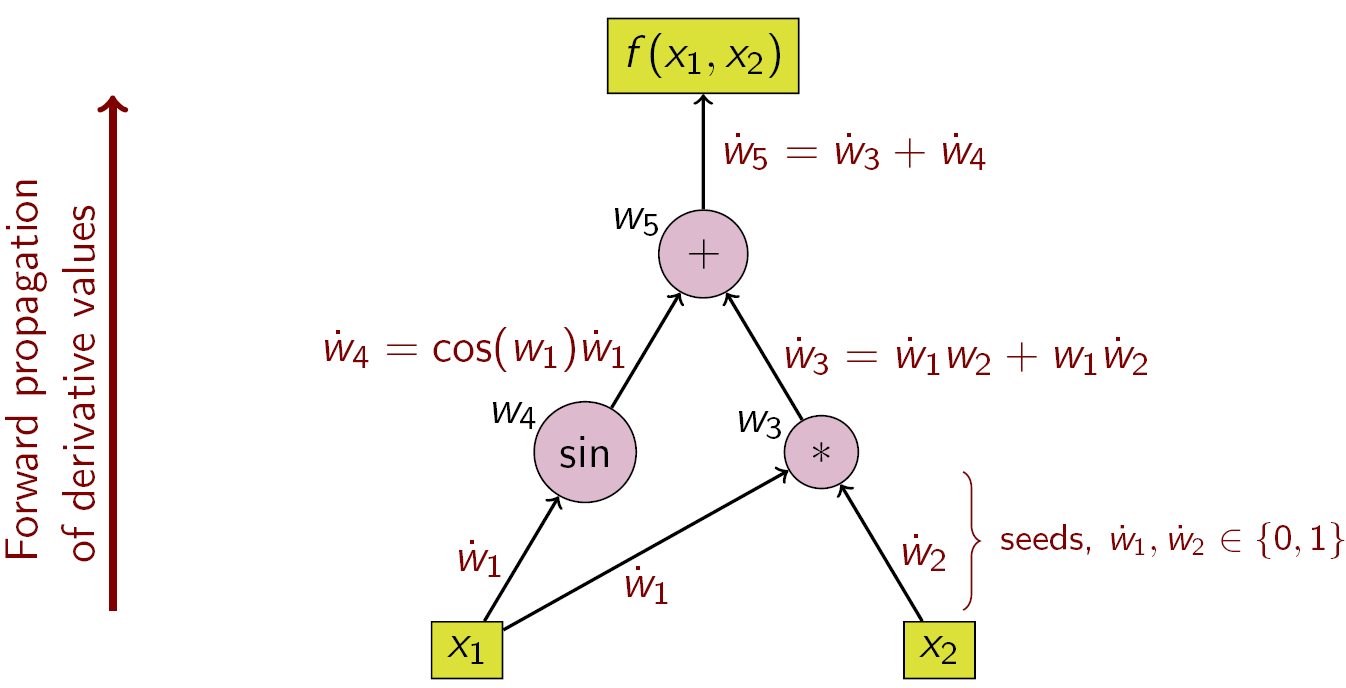
\includegraphics{bilder/ForwardAccumulationAutomaticDifferentiation.png}
\caption{Beispiel für Vorwärtsakkumulation mit Berechnungsgraph}
\end{figure}

\hypertarget{ruxfcckwuxe4rtsmodus}{%
\section{Rückwärtsmodus}\label{ruxfcckwuxe4rtsmodus}}

Bei der Rückwärtsakkumulation ist die Größe von Interesse der \emph{Adjungierte}, bezeichnet mit einem Balken \(\bar{w}_i\); es handelt sich um eine Ableitung einer gewählten abhängigen Variablen in Bezug auf einen Teilausdruck \(w_i\):

\[\bar{w}_i = \frac{\partial y}{\partial w_i}\]

Unter Verwendung der Kettenregel, wenn \(w_i\) Nachfolger im Berechnungsgraphen hat:

\[\bar{w}_i = \sum_{j \in \{\text{Nachfolger von i}\}} \bar{w}_j \frac{\partial w_j}{\partial w_i}\]

Die Rückwärtsakkumulation durchläuft die Kettenregel von außen nach innen oder im Falle des Berechnungsgraphen in Abbildung 3 von oben nach unten. Die Beispiel-Funktion ist skalarwertig, und daher gibt es nur einen Startwert für die Ableitungsberechnung, und nur einen Durchlauf des Berechnungsgraphen ist nötig, um den (zweikomponentigen) Gradienten zu berechnen. Dies ist nur halb so viel Arbeit im Vergleich zur Vorwärtsakkumulation, aber die Rückwärtsakkumulation erfordert das Speichern der Zwischenvariablen \(w_i\) sowie der Anweisungen, die sie erzeugt haben, in einer Datenstruktur, die als ``Band'' oder Wengert-Liste bekannt ist (jedoch veröffentlichte Wengert die Vorwärtsakkumulation, nicht die Rückwärtsakkumulation), was erheblichen Speicher verbrauchen kann, wenn der Berechnungsgraph groß ist. Dies kann bis zu einem gewissen Grad gemildert werden, indem nur eine Teilmenge der Zwischenvariablen gespeichert und dann die notwendigen Arbeitsvariablen durch Wiederholung der Bewertungen rekonstruiert werden, eine Technik, die als Rematerialisierung bekannt ist. Auch das Checkpointing wird verwendet, um Zwischenstände zu speichern.

\begin{figure}
\centering
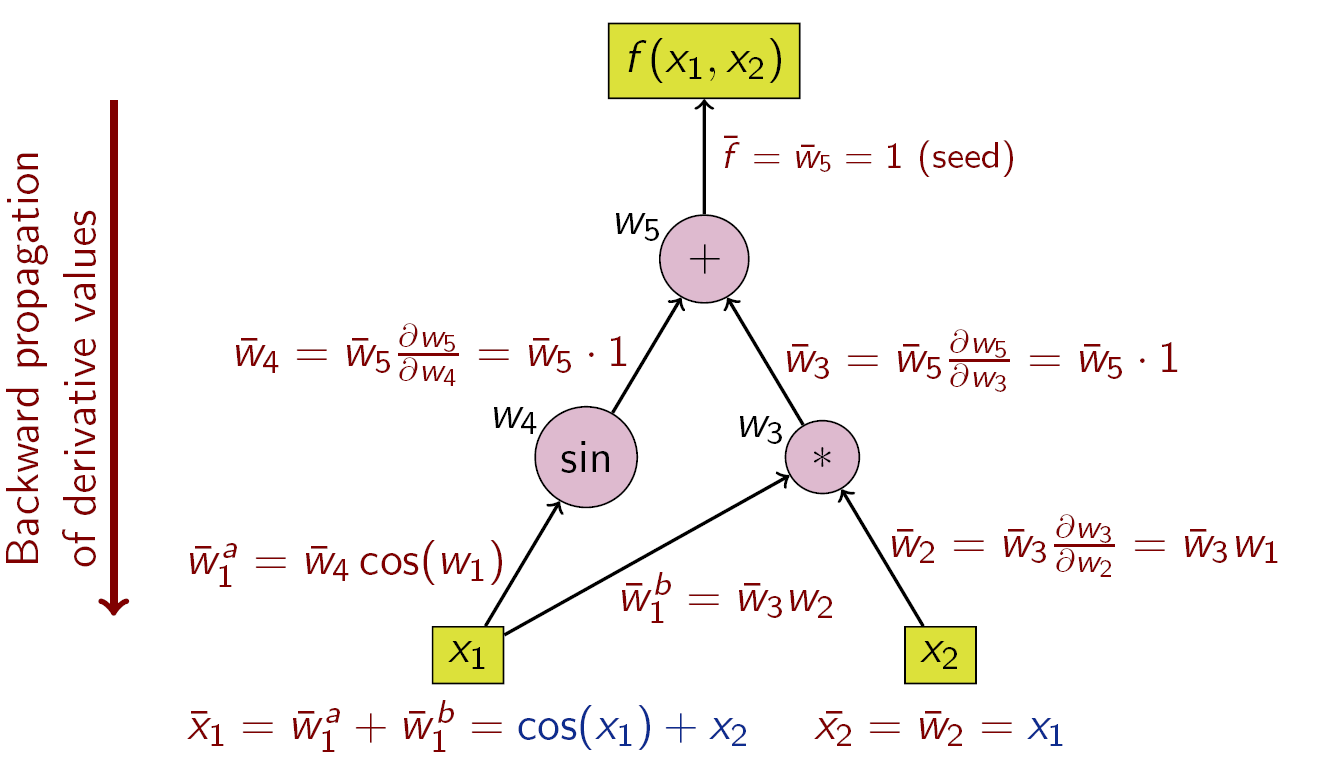
\includegraphics{bilder/ReverseaccumulationAD.png}
\caption{Abbildung 3: Beispiel für Rückwärtsakkumulation mit Berechnungsgraph}
\end{figure}

Die Operationen zur Berechnung der Ableitung mittels Rückwärtsakkumulation sind in der folgenden Tabelle dargestellt (beachte die umgekehrte Reihenfolge):

\begin{itemize}
\tightlist
\item
  \(\bar{w}_5 = 1\) (Startwert)
\item
  \(\bar{w}_4 = \bar{w}_5 \cdot 1\)
\item
  \(\bar{w}_3 = \bar{w}_5 \cdot 1\)
\item
  \(\bar{w}_2 = \bar{w}_3 \cdot w_1\)
\item
  \(\bar{w}_1 = \bar{w}_3 \cdot w_2 + \bar{w}_4 \cdot \cos(w_1)\)
\end{itemize}

Der Datenflussgraph einer Berechnung kann manipuliert werden, um den Gradienten seiner ursprünglichen Berechnung zu berechnen. Dies geschieht durch Hinzufügen eines adjungierten Knotens für jeden primalen Knoten, verbunden durch adjungierte Kanten, die den primalen Kanten parallel verlaufen, aber in entgegengesetzter Richtung fließen. Die Knoten im adjungierten Graphen repräsentieren die Multiplikation mit den Ableitungen der Funktionen, die von den Knoten im primalen berechnet wurden. Zum Beispiel führt Addition im Primalen zu Fanout im Adjungierten; Fanout im Primalen führt zu Addition im Adjungierten; eine unäre Funktion \(y = f(x)\) im Primalen führt zu \(x̄ = ȳ f′(x)\) im Adjungierten; usw.

\hypertarget{implementierungen-anwendungsbeispiele-backpropagation}{%
\chapter{Implementierungen, Anwendungsbeispiele, Backpropagation}\label{implementierungen-anwendungsbeispiele-backpropagation}}

\ldots{}

\hypertarget{nachklapp}{%
\chapter{Nachklapp}\label{nachklapp}}

Ein paar lose Beispiele wo Numerik und maschinelles Lernen sich treffen.

\begin{itemize}
\item
  Iterative Methoden

  \begin{itemize}
  \tightlist
  \item
    Konvergenz/Konvergenzraten
  \item
    stochastische Konvergenz
  \item
    lokale Extrema
  \item
    randomisierte Methoden
  \end{itemize}
\item
  Optimierung/Ausgleichsrechnung
\item
  Approximationstheorie

  \begin{itemize}
  \tightlist
  \item
    Universal Approximation Theorem
  \end{itemize}
\item
  Stabilität und Fehleranalyse

  \begin{itemize}
  \tightlist
  \item
    mixed precision Arithmetik
  \end{itemize}
\item
  Numerische lineare Algebra

  \begin{itemize}
  \tightlist
  \item
    PCA
  \item
    Support Vector Machines
  \item
    Empfehlungssysteme
  \end{itemize}
\item
  Automatisches Differenzieren

  \begin{itemize}
  \tightlist
  \item
    \emph{backward propagation} zur Gradientenberechnung
  \end{itemize}
\end{itemize}

\hypertarget{referenzen}{%
\chapter*{Referenzen}\label{referenzen}}
\addcontentsline{toc}{chapter}{Referenzen}

\hypertarget{refs}{}
\begin{cslreferences}
\leavevmode\hypertarget{ref-BolM04}{}%
Bollhöfer, M., Mehrmann, V.: Numerische Mathematik. Eine projektorientierte Einführung für Ingenieure, Mathematiker und Naturwissenschaftler. Vieweg (2004)

\leavevmode\hypertarget{ref-Byr14}{}%
Byrne, C.L.: Lecture notes on iterative optimization algorithms, \url{https://faculty.uml.edu/cbyrne/IOIPNotesOct2014.pdf}, (2014)

\leavevmode\hypertarget{ref-NocW06}{}%
Nocedal, J., Wright, S.J.: Numerical optimization. Springer (2006)

\leavevmode\hypertarget{ref-RicW17}{}%
Richter, T., Wick, T.: Einführung in die numerische Mathematik. Begriffe, Konzepte und zahlreiche Anwendungsbeispiele. Heidelberg: Springer Spektrum (2017)
\end{cslreferences}

\end{document}
